% ==========================================================================
% The two geographies of urban deprivation — draft manuscript (revision 1)
%
% Drafted from docs/paper-pack/BRIEF.md (final 67-city state, re-anchored
% emergency scale, runs 32012438178 + 32055983121); revised per
% paper/REVISION.md (PI review 2026-08-31). Every number traces to a table
% in docs/paper-pack/data/ or to the depacc-results branch; the
% claim -> table pairing is the brief's evidence map. Cite only from
% references.bib (verified entries; see docs/paper-pack/REFERENCES.md).
%
% Build: latexmk -pdf main.tex   (figures under figures/, includes under
% tables/ regenerated by make_includes.py after any pack refresh; the 2.5
% figure regenerated by make_fig_dep_vs_access.py).
% ==========================================================================
\documentclass[11pt]{article}

\usepackage[T1]{fontenc}
\usepackage[utf8]{inputenc}
\usepackage{lmodern}
\usepackage[a4paper,margin=2.5cm]{geometry}
\usepackage{graphicx}
\usepackage{booktabs}
\usepackage{longtable}
\usepackage{amsmath}
\usepackage{caption}
\usepackage[numbers,sort&compress]{natbib}
\usepackage[hidelinks]{hyperref}

% break long DOIs in the bibliography instead of overflowing the margin
\newcommand{\doi}[1]{doi:~\href{https://doi.org/#1}{\nolinkurl{#1}}}

\graphicspath{{figures/main/}{figures/appendix/}{figures/appendix/cities/}}
\captionsetup{font=small,labelfont=bf}

\newcommand{\gref}{g(15)}          % emergency reporting anchor
\newcommand{\pw}[1]{$p_{\mathrm{wild}} = #1$}
\newcommand{\pperm}[1]{$p_{\mathrm{perm}} = #1$}

\title{\textbf{The two geographies of urban deprivation:\\
everyday services and emergency care in 67 European cities}}

\author{Tina Comes$^{1,\ast}$%
  \\[4pt]
  \small $^{1}$Delft University of Technology, Faculty of Technology, Policy and Management,\\
  \small Delft, The Netherlands\\
  \small $^{\ast}$Corresponding author: \texttt{t.comes@tudelft.nl}\\[2pt]
  \small \emph{[Author list and affiliations to be completed before submission.]}}
\date{Draft of \today}

\begin{document}

\maketitle

% --------------------------------------------------------------------------
\begin{abstract}
\noindent
Cities concentrate people and the infrastructures that sustain them; a
growing share of humanity depends on how well urban systems deliver the
services of daily life and the emergency care on which survival depends. Urban theory
treats access to such services as a quantity that improves predictably
with city size, and measures it in travel minutes applied uniformly across
needs. Yet the welfare burden of poor access is need-specific: it
saturates for substitutable everyday services and escalates without bound
for time-critical care. Here we measure potential deprivation rather than
access, transferring calibrated welfare-loss functions from humanitarian
logistics to a 100\,m population grid covering 67 European functional
urban areas in 24 countries: a bounded deprivation level for everyday
services anchored on the 15-minute-city threshold, and an unbounded
deprivation cost for emergency care anchored on clinical response
benchmarks. The two regimes obey different laws. City size buys everyday
access while emergency deprivation shows no detectable size gradient, and
everyday inequality rises with size while emergency inequality never
falls. Where the regimes diverge is structured by country and macro-region
rather than by size, and the divergence culminates in a severity ordering
of emergency-periphery coverage whose extreme, five capital-city emergency
deserts, is invisible to access averages. The same residents are deprived in
both regimes above chance in 66 of 67 cities, most strongly in
Central-Eastern Europe, and children carry the compounded burden in 88
percent of cities. Urban growth delivers welfare
regime by regime: everyday welfare through agglomeration, emergency
welfare only through coverage.
\end{abstract}

\bigskip
\noindent\textbf{Significance statement.}
Urban scaling theory holds that infrastructure and service provision
improve systematically with city size, and accessibility research measures
that provision in travel minutes. We show that the scaling regularity
governs welfare for only one class of needs. Measuring anchored
deprivation rather than travel time across 67 European city regions,
everyday welfare improves with size while emergency welfare does not, and
inequality in everyday welfare grows with size. Five European capitals
harbour emergency deserts that minutes-based statistics cannot detect, and
children are the most consistent carriers of compounded deprivation.
Welfare-anchored deprivation rather than uniform travel time is the
quantity urban theory should scale, with everyday and emergency capability
entering that theory as separate regimes.

\bigskip
\noindent\textbf{Keywords:} urban scaling; deprivation cost; accessibility;
15-minute city; emergency medical services; spatial equity; resilience

\clearpage

% ==========================================================================
\section{Introduction}\label{sec:intro}
% ==========================================================================

Urban critical infrastructure serves residents on two clocks. On the slow
clock, people choose when to reach a general practitioner, a pharmacy, a
supermarket, a school or a park; these trips recur often, and poor access
to them can be coped with. On the fast clock, an ambulance or an emergency
department must reach a patient, and minutes translate into survival
probabilities. Whether urban growth serves both clocks, and who is left
behind when it serves only one, is a question that sits at the
intersection of three literatures, each of which supplies part of the
answer and none of which can currently pose the question in welfare terms.

The first is urban scaling theory. Since the discovery that diverse urban
quantities follow power laws of population with exponents falling into
universality classes, with socio-economic outputs superlinear and
infrastructure sublinear, scaling theory has treated the returns to city
size as systematic and general \citep{bettencourt2007growth}. Recent work
has begun to condition that generality, showing for instance that the
growth advantage of large cities depends on the urbanisation stage of
their national system \citep{musso2026cities}. For service provision the
scaling account makes a strong implicit prediction: if the returns to
scale that concentrate facilities in larger cities are general, then
access to everyday services and access to emergency care should improve
together with city size. Whether that prediction holds has never
been tested, because the scaling literature measures quantities of
infrastructure rather than the welfare its spatial distribution delivers,
and because it treats all service classes as one.

The second is the accessibility literature. Proximity-based planning
doctrine, most visibly the 15-minute-city programme
\citep{moreno2021fifteenminute,papadopoulos2023compliance}, global
minutes-based accessibility mapping \citep{wu2025global,weiss2020healthcare}
and the measurement of unequal access within cities
\citep{nicoletti2023disadvantaged} have made travel time the common
currency of urban service analysis. That currency embeds a measurement
assumption so familiar it is rarely stated: a minute counts the same
wherever it falls, for whichever service, at whichever point of the
distribution. The assumption is false in both directions at once. For a
substitutable everyday service, the difference between a 25- and a
45-minute walk is largely immaterial, because households reorganise
routines around poor access; for emergency care, the difference between an
8- and a 15-minute response is clinically decisive. A uniform minutes
scale therefore overstates welfare variation where it does not matter and
understates it where it matters most, and any average over such a scale
inherits both errors.

The third literature supplies the correction. Humanitarian logistics has
formalised \emph{deprivation}: the welfare cost of time spent without
access to a good or service, estimable as a function of deprivation time
\citep{holguinveras2013objective,holguinveras2016econometric}. Two objects
emerge from that programme, and their difference carries this paper.
Deprivation from substitutable needs is a \emph{level}: bounded and
S-shaped, saturating once coping sets in \citep{wang2017deprivation}. Deprivation
from critical needs is a \emph{cost}: convex and unbounded, rising ever
more steeply with time, with discrete-choice and stated-preference
estimates available for goods and specifically for emergency ambulance
services
\citep{cantillo2018discrete,macea2018attitudes,delgadolindeman2019ambulance}.
We transfer these functional forms to intra-urban access and calibrate
their curvature to domain anchors: the 15-minute-city threshold for the
everyday level, and the emergency-medical-service (EMS) response
benchmarks for the emergency cost, under which deprivation is negligible
below the 3--4 minute ideal, accumulates through the widely used and
empirically contested 8-minute urban response standard, and reaches the
benchmark cost at the 10--15 minute upper target
\citep{pons2005response,blanchard2012response,peleg2004ems,vo2020vulnerable,khan2026melbourne}.
Throughout the paper, \emph{deprivation level} refers to the bounded
everyday object (1 = full deprivation) and \emph{deprivation cost} to the
unbounded emergency object, reported in multiples of the cost at the
15-minute benchmark; the two are different mathematical objects by design,
and only unit-invariant statistics compare them.

Treating the two regimes as distinct capabilities is also what resilience
theory demands. Resilience has been defined through equitable access to
essential services \citep{logan2020reframing,meerow2016defining}, equality
of access and network resilience have been shown to move together
\citep{fan2022equality}, and everyday vulnerability profiles have been
shown empirically to fail as predictors of crisis-time capability
\citep{sirenko2026heatwaves}. If everyday functioning and emergency
capability are separate dimensions, a city may deliver one and fail the
other, and the population for whom both fail carries a \emph{compounded}
burden that no single-regime statistic reveals. What has been missing is a
comparative measurement of both regimes, in welfare terms, across a
continental urban system.

This paper provides that measurement. We compute the two deprivation
surfaces on a common 100\,m population grid for 67 functional urban areas
(FUAs) in 24 European countries, from 101{,}050 to 12.9 million
inhabitants, drawn by a stratified design over four macro-regions and four
size strata. Following the scaling tradition we estimate log-log
elasticities of city outcomes on population \citep{bettencourt2007growth}
under a harmonised city definition \citep{musso2026cities}. One qualifier
applies to everything that follows and is stated here once: every size
gradient in this paper is cross-sectional, and any phrase such as ``as
cities grow'' means the space-for-time reading of that gradient, never a
longitudinal observation.

Four questions organise the analysis, each aimed at one of the literatures
above. RQ1: do larger cities provide better everyday services and better
emergency capability, in levels and in inequality, as scaling generality
would predict? RQ2: where do the two deprivations diverge, and what
structures the divergence: size, country, region, or coverage? RQ3: who
carries compounding deprivation, in terms of co-location typology and
vulnerability strata? RQ4: what does analysing deprivation add over the
access metrics that currently carry the accessibility literature?

The answers, previewed: agglomeration benefits are regime-specific (size
buys everyday access and no detectable emergency relief, while everyday
inequality rises with size); the divergence is structured by country and
macro-region rather than size, and resolves into a one-dimensional
severity ordering of emergency-periphery coverage whose extreme is five
capital-city emergency deserts; compounding exceeds statistical
independence almost everywhere and falls most consistently on children;
and the deprivation layer changes no rank-based conclusion while halving
unexplained variance and exposing the tail phenomena that access averages
cannot represent. A robustness architecture, combining rank-invariance by
construction, a specification curve, rank-agreement statistics, a
routing-engine cross-check and an access-based re-estimation of every
headline, is reported as a reusable template.

% ==========================================================================
\section{Results}\label{sec:results}
% ==========================================================================

\subsection*{What is measured}

Two surfaces summarise each city; their construction is in Materials and
Methods, and Fig.~\ref{fig:curves} shows the welfare logic that
distinguishes them. The \emph{everyday deprivation level} of a grid cell,
between 0 and 1, expresses how far the burden of reaching five everyday
service categories on foot has progressed toward saturation: near 0, all
services are comfortably walkable; near 1, the cell is effectively without
walkable everyday services and additional minutes no longer add burden.
The \emph{emergency deprivation cost} of a cell is an open-ended positive
number expressing the welfare cost of its drive time to the nearest
emergency facility, in multiples of the cost at the 15-minute EMS
benchmark: a cell at 2.0 carries twice the deprivation cost of one whose
ambulance arrives at the benchmark, and the cost keeps escalating beyond
it. Both curves are anchored on external standards rather than fitted to
the data, and the linear loss that any minutes average implicitly applies
is drawn beside them in Fig.~\ref{fig:curves}: relative to the calibrated
curves, the linear loss over-prices minutes where they are welfare-inert
(the saturated everyday range) and under-prices them where they are
clinically decisive (around the emergency benchmarks).

\begin{figure}[t]
\centering

\includegraphics[width=.95\textwidth]{deprivation_curves.png}
\caption{What matters, by regime: the two calibrated deprivation functions
and the linear loss a minutes average implies. Left: everyday deprivation
level (logistic, inflection at the 15-minute anchor; Layer-1 curvature
sweep; concave Box-Cox form swap dashed), on its own 0--1 scale. Centre:
emergency deprivation cost (convex Box-Cox, $\lambda = 1.8$, in multiples
of \gref{}) inside the benchmark window, where all forms coincide at the
EMS anchors by construction (negligible at 4 min; $\approx$0.35 at the
contested 8-min standard; 1 at the 15-min target). Right: beyond the
15-minute cut-off no benchmark exists and the three literature-grounded
escalation hypotheses diverge (at 60 min: 1.61$\times$ saturating,
11.2$\times$ polynomial baseline, 120$\times$ exponential; log scale). The
dotted line in each panel is the linear loss of a pure-access average.
Each panel stays on its own reporting scale; panels are never compared in
magnitude.}
\label{fig:curves}
\end{figure}

The bounded level and the unbounded cost are deliberately different
objects, because the needs are: everyday services are substitutable, so
their deprivation saturates; emergency care is time-critical, so its
deprivation escalates. Forcing both into levels would assert that a
60-minute ambulance is no worse than a 30-minute one; forcing both into
costs would assert that living far from a supermarket is unboundedly
catastrophic. The asymmetry is the substantive claim about what matters,
and it imposes one discipline used throughout: only unit-invariant
statistics cross regimes (elasticities, Ginis, rank-based measures), and
raw magnitudes never do.

Table~\ref{tab:sample} summarises the sample; Table~\ref{tab:si-cities} in
the SI lists every city. Fig.~\ref{fig:cityplane} gives the overview of
all 67 cities: each city is a point in the plane spanned by its
within-city inequality (Gini) of everyday and of emergency deprivation,
with whiskers spanning the min--max envelope over the
deprivation-curvature sensitivity grid, so each city is placed at the
precision the calibration actually supports. Because cities nest in 24
countries, every scaling claim below cites a wild cluster bootstrap
p-value on country clusters and every regional contrast a
country-permutation p-value; the inference conventions are in Materials
and Methods.

\begin{table}[t]
\centering
\caption{Sample composition and median city indicators by macro-region.
67 functional urban areas (Eurostat/OECD definition: city plus commuting
zone), stratified draw over 4 macro-regions $\times$ 4 size strata
($10^5$--$2.5\cdot10^5$, $2.5\cdot10^5$--$10^6$, $10^6$--$5\cdot10^6$,
$>5\cdot10^6$ inhabitants; 15/18/30/4 cities), 113.9 million residents in
total. $\bar D_{\mathrm{ev}}$: population-weighted mean everyday
deprivation level (0--1); $\bar C_{\mathrm{em}}$: mean emergency
deprivation cost (multiples of \gref{}; not comparable to
$\bar D_{\mathrm{ev}}$ in magnitude); $G$: within-city population-weighted
Gini; $\rho$: Spearman rank coupling of the two surfaces; HH: compounding
population share at the median split. Source:
\texttt{cities\_descriptives.csv}.}
\label{tab:sample}
\small
\begin{tabular}{@{}lrrrrrrrrr@{}}
\toprule
Region & Cities & Countries & Pop.\ (M) & $\bar D_{\mathrm{ev}}$ &
$\bar C_{\mathrm{em}}$ & $G_{\mathrm{ev}}$ & $G_{\mathrm{em}}$ & $\rho$ & HH \\
\midrule
North  & 13 & 4  & 11.3 & 0.41 & 1.81 & 0.39 & 0.47 & 0.47 & 0.34 \\
West   & 16 & 5  & 37.1 & 0.23 & 0.74 & 0.52 & 0.41 & 0.36 & 0.32 \\
South  & 18 & 4  & 39.8 & 0.29 & 1.07 & 0.42 & 0.42 & 0.38 & 0.32 \\
CEE    & 20 & 11 & 25.6 & 0.30 & 1.48 & 0.51 & 0.54 & 0.55 & 0.36 \\
\midrule
All    & 67 & 24 & 113.9 & 0.29 & 1.14 & 0.49 & 0.44 & 0.42 & 0.33 \\
\bottomrule
\end{tabular}
\end{table}

\begin{figure}[t]
\centering

\includegraphics[width=\textwidth]{cityplane.png}
\caption{All 67 cities in the inequality plane. Horizontal axis:
within-city Gini of the everyday deprivation level; vertical axis:
within-city Gini of the emergency deprivation cost. Whiskers span the
min--max envelope of each Gini over the deprivation-curvature sensitivity
grid (Section~\ref{sec:robust}). Colours mark macro-regions; the
emergency-desert group of Section~\ref{sec:geography} is outlined.}
\label{fig:cityplane}
\end{figure}

% --------------------------------------------------------------------------
\subsection{City size buys everyday access; emergency relief shows no
detectable size gradient}\label{sec:scaling}

If the returns to scale behind urban service provision were general, as
the universality claims of scaling theory suggest for infrastructure
\citep{bettencourt2007growth}, both deprivations should fall with city
size. The everyday regime behaves exactly as that account predicts. Mean
everyday deprivation falls systematically with population
(Fig.~\ref{fig:scaling}): the log-log elasticity is $-0.196$
(country-clustered SE 0.023, \pw{0.0002}), meaning mean everyday
deprivation falls by roughly 19\,\% for each e-fold ($\approx 2.7\times$)
of population, and city size alone explains 44\,\% of the cross-city
variance ($R^2 = 0.44$). The mechanism is visible in the descriptive
layer beneath the deprivation surfaces: the median FUA routes its
population to 93 mapped general practitioners, 228 pharmacies, 325
supermarkets, 409 schools and 636 green spaces, and the
population-weighted median walk to the nearest facility of each everyday
category is 4--8 minutes; larger cities carry denser facility networks,
and the deprivation level converts that density into welfare terms.

The estimate survives every diagnostic we throw at it. It is stable under
country fixed effects ($-0.17$), under leave-one-out city deletion
(envelope $-0.204$ to $-0.185$, with Athina the most influential city),
under outlier-robust estimators (Huber $-0.196$, median regression
$-0.223$) and under exclusion of the five emergency-desert capitals
($-0.203$), so no single city, country or estimator choice carries it.

The emergency regime breaks the pattern. Mean emergency deprivation cost
shows no detectable size gradient: the elasticity is $-0.059$ (clustered
$p = 0.16$, \pw{0.21}), and city size explains 2\,\% of the cross-city
variance. Non-significance alone would be weak evidence, so the null is
bounded: two one-sided equivalence tests place the emergency elasticity
within $\pm 0.13$ \citep{lakens2017equivalence}. The bound licenses a
precise statement and no more: any emergency size gradient, if present, is
at most two-thirds the everyday one in magnitude; equivalence at the
stricter $\pm 0.10$ bound is not shown, so the claim is ``no detectable
scaling, bounded within $\pm 0.13$'', never ``proven flat''. The
descriptive layer again shows why: the median FUA has 6 emergency
departments and 6 ambulance stations for its whole territory, the median
population-weighted drive to either is 12 minutes, and the facility count
of a national emergency system does not multiply with city population the
way pharmacies do.

The two slopes also differ from each other, tested within cities rather
than by comparing two separate regressions: a paired regime test
(regime $\times$ log-population interaction, country-clustered) puts the
everyday slope $0.137$ below the emergency slope (\pw{0.002}). RQ1's
level half therefore has a clean answer: agglomeration benefits are
regime-specific. Bigger cities deliver everyday services closer to
people; proximity to emergency care does not improve detectably with
size, and the difference between the regimes is itself significant. For
scaling theory the implication is direct: the returns to scale that
govern everyday provisioning do not extend across service classes, so no
single exponent describes what city size does to service welfare.

\begin{figure}[t]
\centering

\includegraphics[width=.9\textwidth]{scaling_elasticity.png}
\caption{Regime-specific agglomeration. Population-weighted mean
deprivation against FUA population (log-log) for both regimes across the
67 cities; the two series are in different units (everyday: level 0--1;
emergency: cost in multiples of \gref{}), so only the slopes compare,
never the levels. Everyday deprivation level: elasticity $-0.196$,
country-clustered wild bootstrap $p = 0.0002$, $R^2 = 0.44$. Emergency
deprivation cost: elasticity $-0.059$, wild $p = 0.21$, bounded within
$\pm 0.13$ by equivalence testing. The paired slope difference of
$+0.137$ is significant at wild $p = 0.002$. Gradients are
cross-sectional (space-for-time).}
\label{fig:scaling}
\end{figure}

% --------------------------------------------------------------------------
\subsection{Inequality scales with size only in the everyday
regime}\label{sec:inequality}

Within-city inequality answers RQ1's second half, and it inverts the
comfort of the first. The Gini of everyday deprivation rises with
population: elasticity $+0.062$ (\pw{0.0012}). The emergency Gini is
size-flat at the baseline parameterisation ($+0.004$, \pw{0.84}), and the
paired slope difference of $-0.058$ is significant over all 67 cities
(\pw{0.029}). Size therefore buys mean everyday access at the price of a
wider spread around that mean, while emergency inequality is set
elsewhere. The everyday half of the claim is defended by a specification
curve \citep{simonsohn2020specification} rather than by any single
calibration (Fig.~\ref{fig:speccurve}): re-estimating the slope under all
14 deprivation parameterisations (the curvature grid and the
functional-form swaps of Section~\ref{sec:robust}) keeps it positive
throughout ($+0.026$ to $+0.075$) and significant in 13 of 14. The
exception is the concave Box-Cox everyday form swap ($+0.026$,
$p = 0.083$), which we state rather than smooth over.

The emergency half is conditional, and we report the conditionality as a
finding rather than resolve it by choice of parameterisation. The EMS
benchmarks define the cost scale up to the 15-minute cut-off, and all
three literature-grounded escalation forms are calibrated to coincide
there. Beyond the cut-off no benchmark exists, and that is exactly where
the forms diverge (Fig.~\ref{fig:curves}, right panel). Under the bounded
survival-based curve (1 = full deprivation, saturating around 30--45
minutes) the emergency Gini is size-flat ($+0.001$, $p = 0.97$). Under
polynomial Box-Cox escalation, the published baseline, it is size-flat
across the whole curvature sweep ($-0.006$ to $+0.014$, none
significant), in agreement with the deprivation-free travel-time Gini,
itself size-flat ($-0.015$, $p = 0.42$). Under exponential escalation the
Gini rises with size ($+0.098$, $p = 0.0003$); the mechanism, verified in
the data, is that exponential pricing turns the Gini into an index of
extreme-tail depth (it saturates at a median of 0.96, decouples from the
time distribution's inequality, $\rho = 0.04$, and tracks the
beyond-45-minute population share, $\rho = 0.45$), and how many minutes
past the cut-off the worst-served residents sit does grow with size, even
though the tail's population share does not (beyond-30-minute share
elasticity $-0.003$, $p = 0.99$). Two statements hold under every
parameterisation: everyday inequality rises with size, and emergency
inequality never falls with size. Whether emergency inequality is flat or
rising is decided by the beyond-benchmark escalation form, which no
clinical benchmark pins down; it is flat under two of the three
hypotheses and rising under the third.

\begin{figure}[t]
\centering

\includegraphics[width=.95\textwidth]{specification_curve.png}
\caption{Specification curve of the inequality-scaling slopes. Top:
everyday Gini; bottom: emergency Gini. Each point is the size elasticity
of the within-city Gini re-estimated under the ringed baseline or one of
the 14 alternative deprivation parameterisations (blue: curvature grid;
orange: functional-form swaps); whiskers are country-clustered 95\,\%
CIs. The everyday-Gini slope is positive under every specification
($+0.026$ to $+0.075$; significant in 13/14, the exception being the
concave Box-Cox form swap at $p = 0.083$). The emergency-Gini slope
splits by beyond-cut-off escalation form: flat under saturating and
polynomial escalation, rising only under exponential escalation
($+0.098$, $p = 0.0003$).}
\label{fig:speccurve}
\end{figure}

% --------------------------------------------------------------------------
\subsection{The geography of divergence: country-level structure and a
coverage gradient}\label{sec:geography}

If size does not set emergency deprivation, what does? The divergence
between regimes has a geography, and the honest unit for testing it is
the country: macro-region is a property of countries, so whole countries
are permuted across regions (Fig.~\ref{fig:regions}). The emergency Gini
differs by macro-region (Cohen $f = 0.74$, \pperm{0.0024}), as do the
divergence gap (\pperm{0.010}), the everyday--emergency coupling $\rho$
(\pperm{0.0015}) and both compounding measures (\pperm{0.0008} for the HH
share, \pperm{0.0023} for the continuous intensity). Central-Eastern
Europe compounds: the region pairs the highest emergency inequality
(median emergency Gini 0.54) with the strongest coupling between the two
surfaces (median $\rho = 0.55$), so the same populations tend to carry
both deprivations. The West's inequality problem is everyday-side (median
divergence gap $-0.12$); the North's is emergency-side ($+0.09$). The
everyday Gini's apparent regional contrast does not survive country-level
testing (\pperm{0.27} despite a city-level ANOVA $p = 0.0007$), a
cautionary illustration of why city-level inference over-claims here.

\begin{figure}[t]
\centering

\includegraphics[width=.95\textwidth]{region_strips.png}
\caption{Regional structure of the divergence: strip plots by
macro-region (bar = regional median) for the coupling $\rho$, the
everyday Gini, the emergency Gini and the divergence gap. Contrasts that
survive country-permutation testing: emergency Gini (\pperm{0.0024}),
divergence gap (\pperm{0.010}), coupling $\rho$ (\pperm{0.0015}); the
compounding measures, tested in the text, also differ regionally (HH
share \pperm{0.0008}; continuous intensity \pperm{0.0023}). The everyday
Gini's apparent contrast does not survive country-level testing
(\pperm{0.27}) and is shown without a claim. Region is a property of
countries, so whole countries are permuted across regions; city-level
p-values would be anti-conservative.}
\label{fig:regions}
\end{figure}

Do the 67 cities fall into types? No. k-means clustering on the full
standardised city-vector separates 62 cities from 5 (silhouette 0.65,
bootstrap ARI 0.87 \citep{hubert1985comparing,rousseeuw1987silhouettes},
Gaussian-null $p = 0.001$), and the isolated group is an outlier group
rather than a typology: its agreement with the region partition is
ARI $= 0.001$. Those five are Bucure\c{s}ti, R\={\i}ga, Vilnius, Tallinn
and Ljubljana, the emergency-desert capitals, separated by their
beyond-threshold emergency travel-time tails. Ward clustering selects the
same axis and cuts it more conservatively, isolating a nested subset of
the two most extreme capitals (65/2). The nesting is evidence for a
gradient: the two algorithms disagree about where to cut a severity
ordering, and agree on the ordering itself. Re-clustering with the
outliers removed finds one further split along the same axis at lower
intensity: a 48/14 cut isolating partial-desert cities with real
emergency tails (among them Oslo, Stockholm, Warszawa, Sofia, Zagreb,
Palermo and Luxembourg; silhouette 0.38, bootstrap ARI 0.74, null
$p = 0.001$, ARI vs region 0.07), inside which Ward again nests (56/6). A
feature-set robustness check that re-runs the whole pipeline with the
8/15-minute benchmark shares added reproduces the main partition exactly
(ARI 1.00) and the peeled cut at ARI 0.97, while flagging Br\u{a}ila and
\L{}om\.za, the two smallest CEE cities, as sitting on the
covered/partial boundary; the same two cities sat on the covered side
under the pre-refresh extraction state. The citable structure is
therefore a one-dimensional \emph{severity ordering} of
emergency-periphery coverage, covered (48) $\rightarrow$ partial desert
(14) $\rightarrow$ desert (5), with a soft boundary between covered and
partial and a robust ordering; we refer to these as coverage grades and
never as city types.

The coverage grade, and no other variable we test, sets the emergency
level. In a single country-clustered model with ln population centred at
the sample mean, the grade dummies shift mean emergency deprivation
overwhelmingly (Wald $p \approx 1.3\times10^{-15}$); the median mean cost
rises 1.02 $\rightarrow$ 1.87 $\rightarrow$ 3.37 multiples of \gref{}
across covered $\rightarrow$ partial $\rightarrow$ desert
(Fig.~\ref{fig:grade}). The slope-by-grade interaction is $p = 0.010$
under the current 48/14/5 grades but was $p = 0.17$ under the pre-refresh
50/12/5 grades; a two-city boundary change flips it, so we treat the
interaction as boundary-sensitive and do not headline any grade-specific
size gradient. The level statement carries the content: coverage class,
not city size, sets emergency deprivation. Consistent with this, the
divergence-gap measures show at most a weak size gradient (gap slope
$-0.066$ per $\log_{10}$ population, $p = 0.012$, $R^2 = 0.06$; Fig.~S2),
so size is a poor predictor of where the two regimes part ways (RQ2).
What the deserts mean, and why access statistics cannot see them, is
taken up in Section~\ref{sec:depvsaccess}.

\begin{figure}[t]
\centering
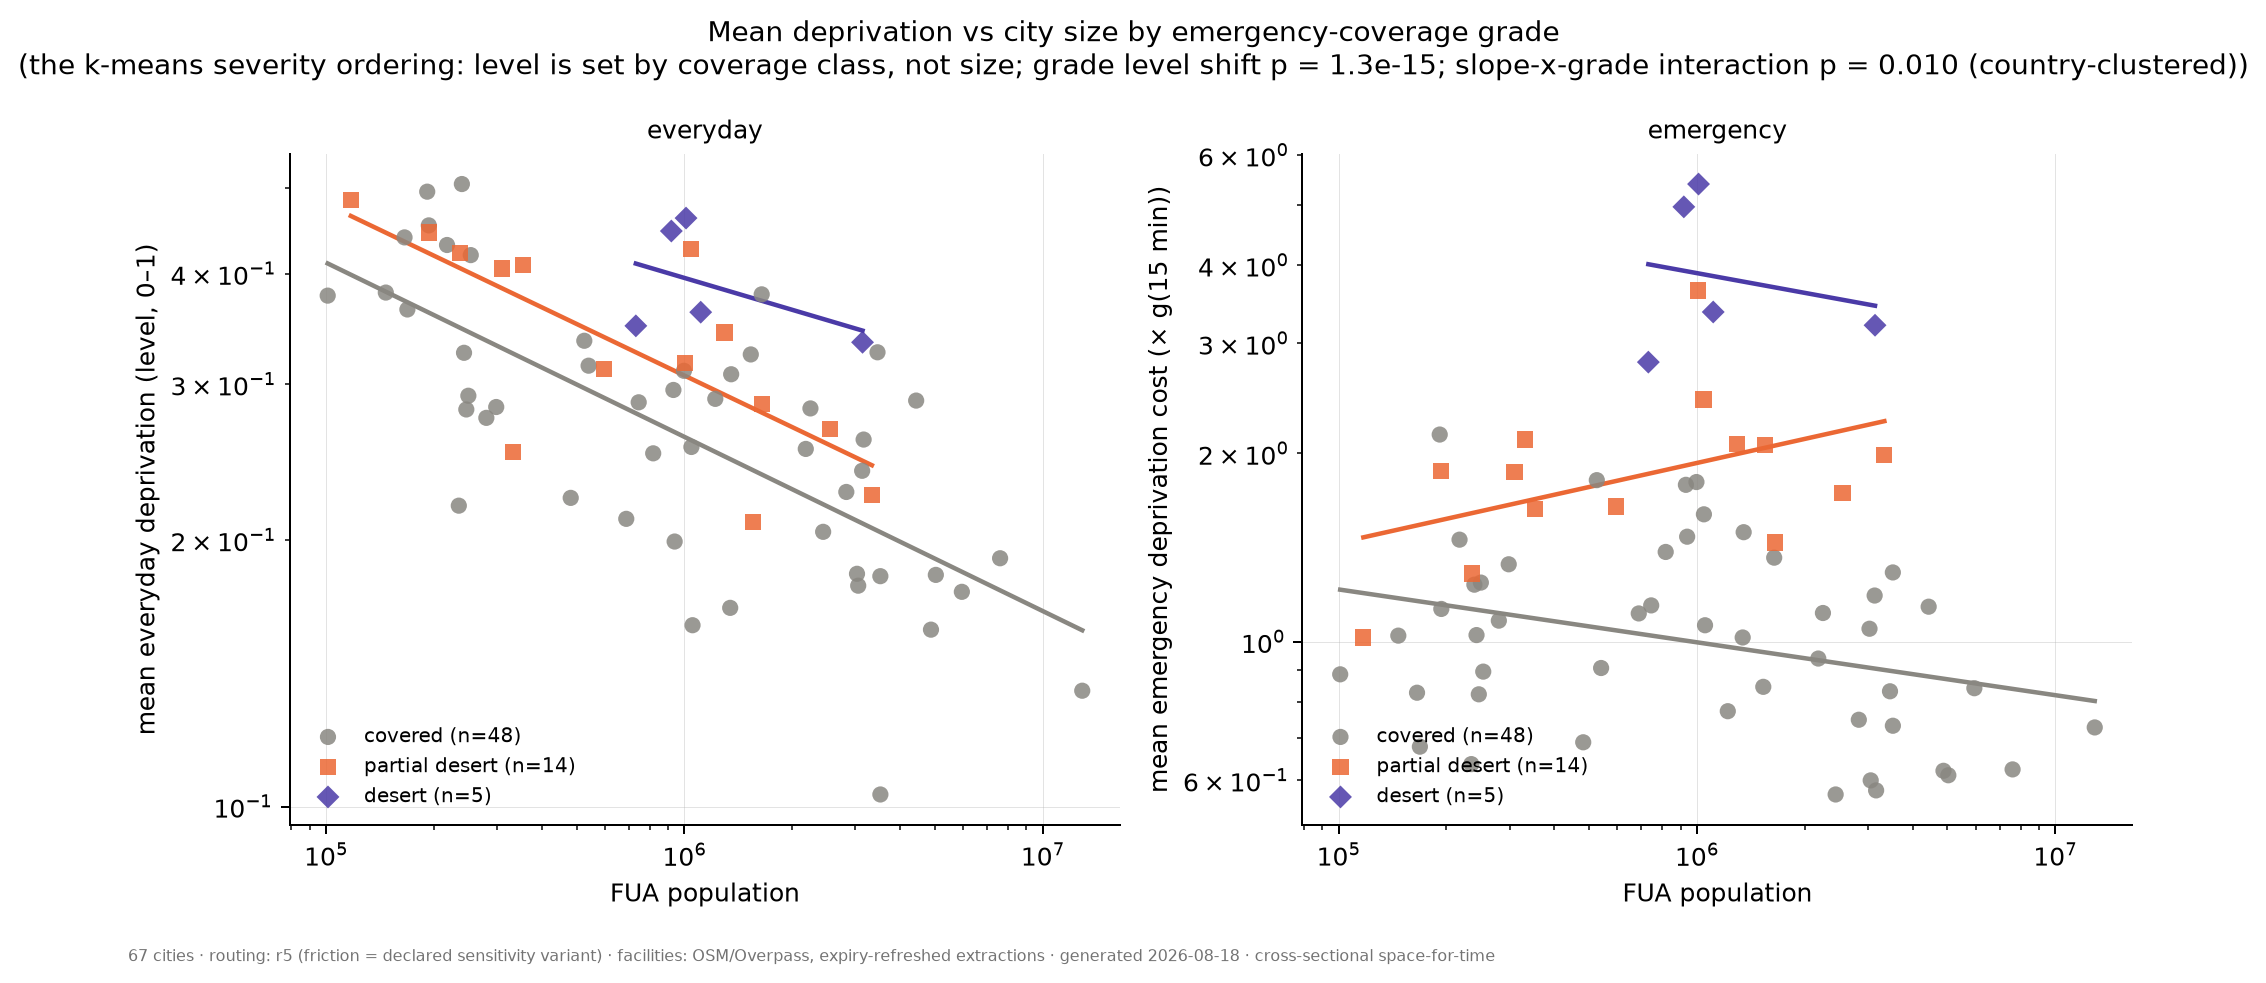
\includegraphics[width=.95\textwidth]{scaling_by_coverage_grade.png}
\caption{Mean deprivation against city size by emergency-coverage grade,
per regime (left: everyday level; right: emergency cost, multiples of
\gref{}), grades read from the two clustering passes (covered 48 /
partial desert 14 / desert 5). On the emergency side the grade shifts the
level decisively (country-clustered Wald
$p \approx 1.3\times10^{-15}$; median levels 1.02\,/\,1.87\,/\,3.37),
while the slope-by-grade interaction is boundary-sensitive and not
headlined. Within-grade fits are plain OLS over few cities, shown for
orientation only.}
\label{fig:grade}
\end{figure}

% --------------------------------------------------------------------------
\subsection{Compounding is the norm, and children carry
it}\label{sec:compounding}

How often do the same residents lose on both clocks (RQ3)? The
co-location typology cuts both percentile surfaces at their
population-weighted medians, which fixes the marginals at one half each;
the whole 2$\times$2 class table then has a single free number, the
high-high (HH) compounding share, and statistical independence of the two
surfaces corresponds to HH $= 25\,\%$. Everything above 25\,\% is excess
co-location. The observed HH share averages 33\,\% and exceeds
independence in 66 of 67 cities; the rank coupling $\rho$ between the two
surfaces spans $-0.02$ to $0.74$ (Fig.~\ref{fig:rho}). Compounding is not
an exotic overlap of two rare conditions; across urban Europe it is the
default relationship between the two deprivations.

Thresholded shares invite the question of the threshold, so the
robustness harness prices it: the ``how high is high'' percentile cut
moves the HH share by 29.8 percentage points at the median city, against
1.4 under the whole deprivation-curvature grid and 0.9 under the
functional-form swaps, a roughly 21-fold dominance of the analyst's
threshold over the welfare calibration. Two consequences follow. First,
the headline compounding measure is the threshold-free continuous
intensity, the population-weighted mean depth to which the typical
resident sits inside \emph{both} percentile distributions, with fixed
anchors (1/3 under independence, 1/2 under perfect coupling, 1/4 under
perfect divergence); it shows the same regional structure as the
thresholded share (\pperm{0.0023}, strongest in Central-Eastern Europe).
Second, every thresholded share in this paper travels with its threshold
sweep. The spatial anatomy is consistent across contrasting cities
(Fig.~\ref{fig:gallery}): compounding concentrates in peripheries where
the saturated everyday level meets the escalating emergency cost, while
dense cores hold most population in the low-low class. The maps are read
under two rules stated once: legends carry population-weighted shares
while the picture is area-weighted (a sparse periphery dominates visually
at a modest population share), and no single cell's class is a finding
(roughly 24\,\% of population flips class between routing engines); the
per-city maps for all 67 cities are in the SI gallery.

\begin{figure}[t]
\centering

\includegraphics[width=.9\textwidth]{rho_ranked.png}
\caption{Coupling of the two deprivation surfaces across the 67 cities.
Spearman $\rho$ between the everyday and emergency population-weighted
percentile surfaces, cities ranked; $\rho$ spans $-0.02$ to $0.74$.
Colours mark macro-regions; the emergency-desert capitals are outlined.
The HH compounding share exceeds the 25\,\% independence benchmark in 66
of 67 cities (sample mean 33\,\%). Rank-based measures are invariant to
the deprivation parameterisation.}
\label{fig:rho}
\end{figure}

\begin{figure}[t]
\centering
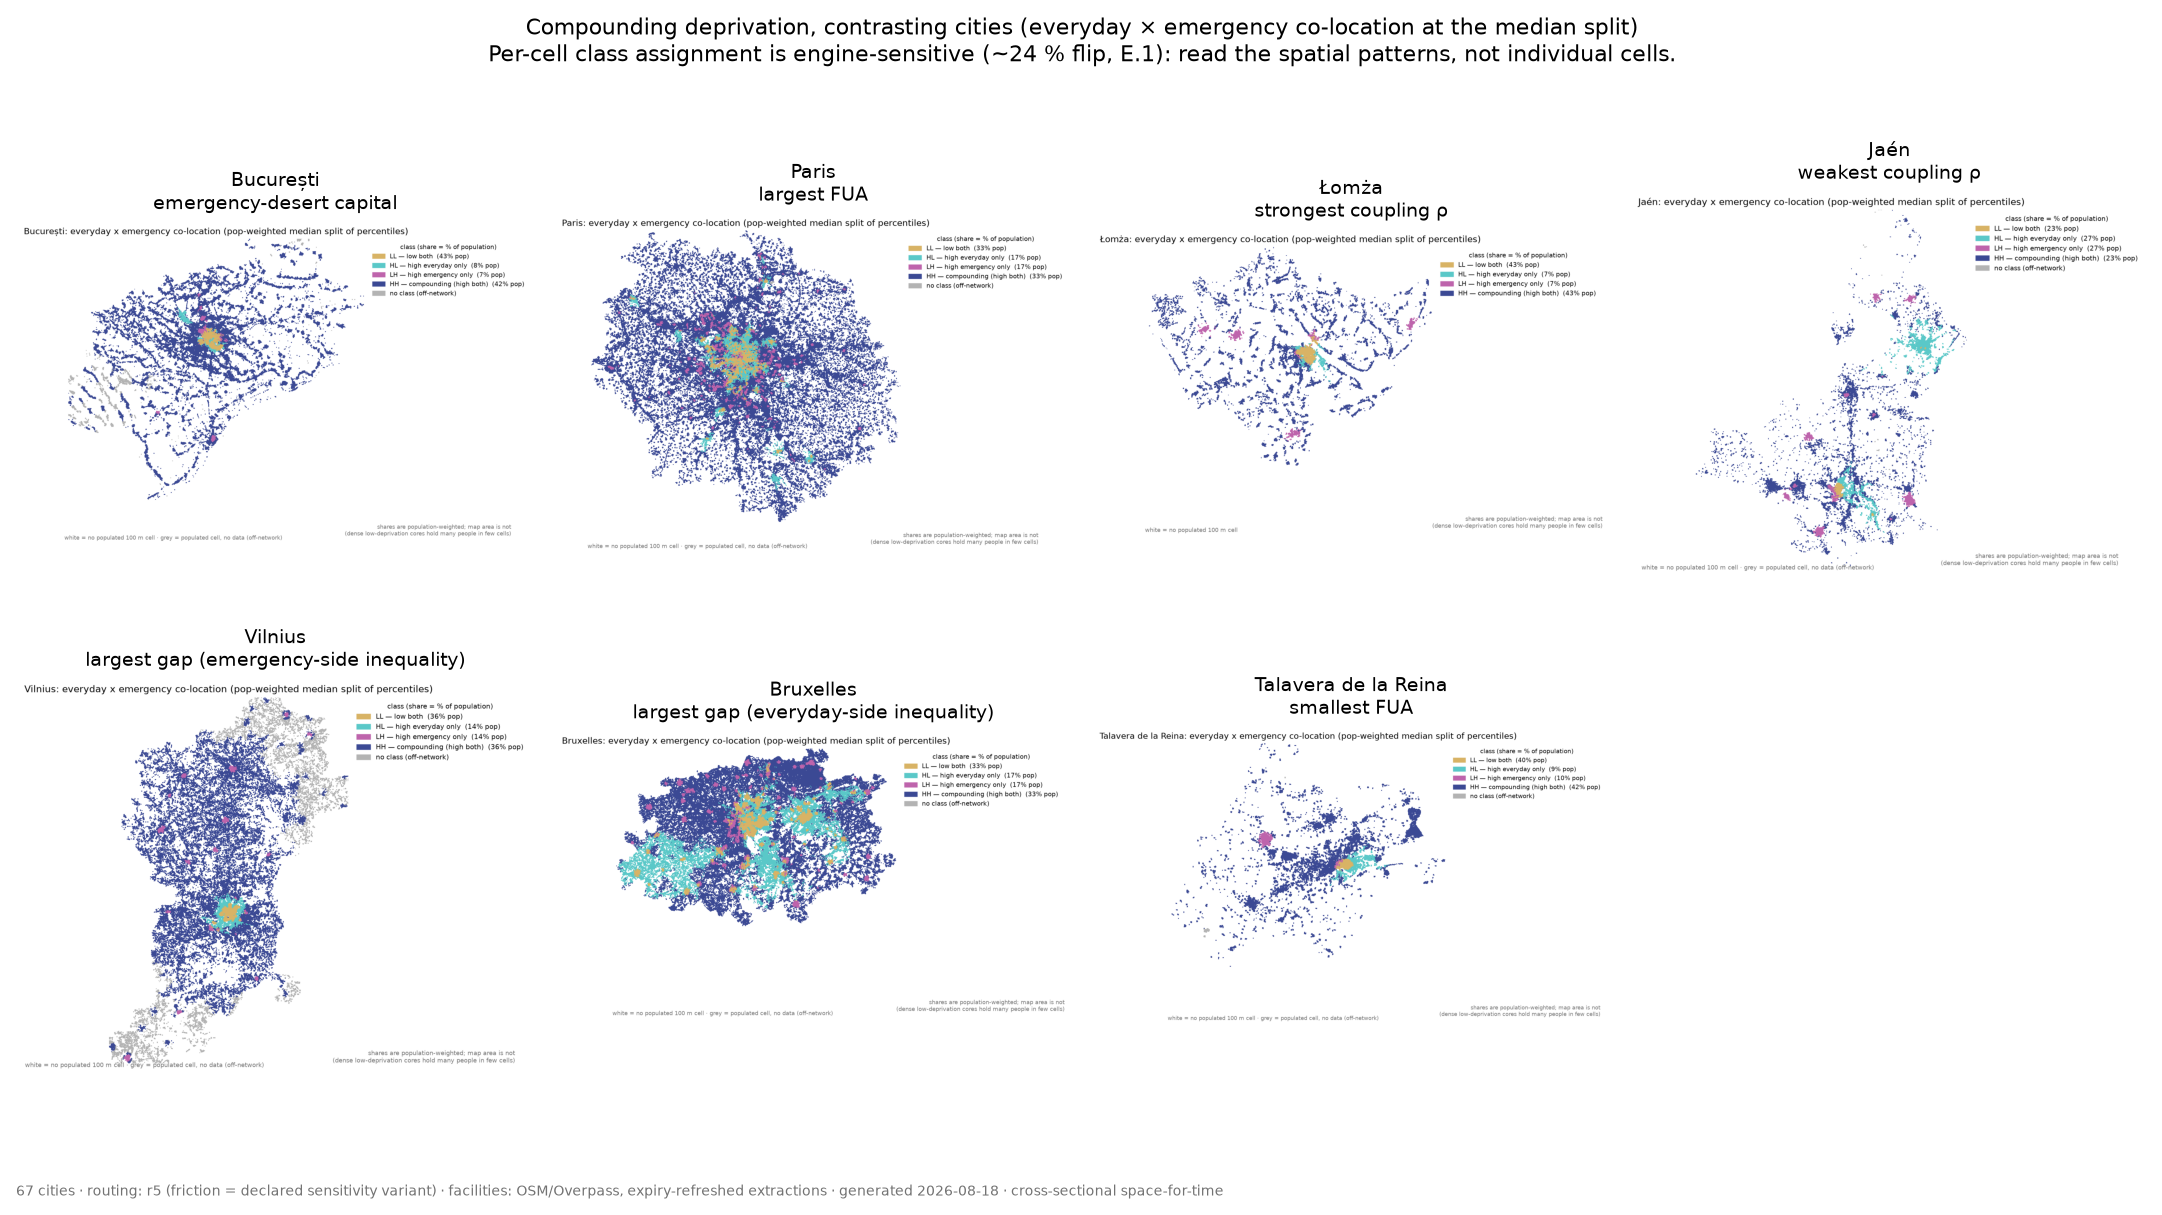
\includegraphics[width=\textwidth]{compounding_gallery.png}
\caption{Compounding gallery: median-split co-location typology for
contrasting cities, each panel labelled with the role it illustrates (all
67 maps in the SI). Colours: LL both low, HL high everyday only, LH high
emergency only, HH compounding. Shares in the
legends are population-weighted; the maps are area-weighted, so a sparse
periphery dominates visually at a modest population share. Maps are read
for spatial pattern only: roughly 24\,\% of population flips class
between routing engines, so no per-cell class is a finding.}
\label{fig:gallery}
\end{figure}

Who lives in the compounded areas? Vulnerability enters on two strictly
separated levels: EU-harmonised census age strata, comparable across all
67 cities and pooled; and national fine-grid strata (rent, tenure, finer
ages), which are per-city depth and never pooled. Each stratum is
compared against the cells where its own census variable is published
(the covered-cell reference), because data coverage has its own
geography. At the harmonised level the result is stark and one-sided:
cells in the top quartile of child share carry more everyday deprivation
than their comparison cells in 88\,\% of cities (median ratio 1.27) and
more compounding in 88\,\% (median HH-share gap $+0.13$), strongest in
Central-Eastern Europe (median ratio 1.44) and the North (1.30)
(Fig.~\ref{fig:vuln}). The elderly show no such pattern at the European
level: median ratio 0.96, above parity in only 37\,\% of cities, below
parity across most of Central-Eastern Europe. That null is itself a
result, and it is scale-specific: the national-data tier resolves sharper
per-city patterns (in Hamburg, elderly 1.37, children 1.52, low-rent 1.61
against covered references), but those use different definitions and
stay per-city. The European claim is about children; whatever sorting
mechanism places families with children in the compounded periphery
operates consistently across nearly the whole sample, in a group whose
daily radius is short and whose emergency risk is real.

\begin{figure}[t]
\centering

\includegraphics[width=.95\textwidth]{vulnerability_strata.png}
\caption{Who carries the deprivation: census-harmonised vulnerability
strata by macro-region, pooled across the 67 cities against covered-cell
references (dashed line = parity; bar = regional median). Columns:
elderly and children strata; top row: everyday deprivation ratio
(stratum vs reference); bottom row: compounding (HH) share gap. Children
(top-quartile child-share cells) experience higher everyday deprivation
in 88\,\% of cities (median ratio 1.27) and higher compounding in 88\,\%
(median HH gap $+0.13$), strongest in CEE (1.44) and the North. The
elderly stratum sits at parity (median 0.96, above 1 in 37\,\% of
cities); no European elderly claim is made. National fine-grid strata
are per-city depth and are never pooled with these.}
\label{fig:vuln}
\end{figure}

% --------------------------------------------------------------------------
\subsection{What deprivation adds over access}\label{sec:depvsaccess}

The framework's value has to be demonstrated against the state of the
art, so every headline regression is re-estimated on the
deprivation-free, minutes-based indicators the accessibility literature
would use \citep{nicoletti2023disadvantaged,wu2025global}, and the answer
to RQ4 comes in three moves (Fig.~\ref{fig:depvsaccess}; exact values in
Table~\ref{tab:si-depvsaccess}).

First, the claims survive dropping the deprivation layer entirely, which
is what protects them from the suspicion of being calibration artefacts.
The everyday size gradient is present in plain minutes (median walk time
elasticity $-0.237$, $p = 3.8\times10^{-5}$; mean walk time $-0.178$),
and the emergency non-gradient is present in minutes too (elasticities
$-0.043$ to $-0.059$ across median, mean and p90 drive time). No headline
of Sections~\ref{sec:scaling}--\ref{sec:geography} depends on the
deprivation functions; the functions restate in welfare terms a structure
the network geometry already carries. One detail of the minutes family
already points at where that structure lives: the only minutes-based
emergency statistic to reach conventional significance is the p90 drive
time ($-0.059$, $p = 0.017$), the most tail-sensitive access statistic in
the set. Even inside the access paradigm, whatever signal the emergency
regime carries sits in the tail of the distribution rather than at its
centre, which is precisely the region a convex cost function is built to
price and an average over uniform minutes is built to dilute.

Second, the deprivation outcome is the better-behaved scientific object
(Fig.~\ref{fig:depvsaccess}A). City size explains 44\,\% of the variance
in mean everyday deprivation against 16\,\% for the median walk minute,
its access counterpart, because the saturating level function discounts
exactly the variation that carries no welfare content: whether a
periphery cell sits 50 or 70 minutes from a pharmacy moves a minutes
average and moves no household's daily reorganisation. Anchored
deprivation acts as a welfare-weighted filter on travel time, and the
filtered outcome is the one that scales cleanly. The filtering costs
nothing in ordering: the deprivation-based and time-based Gini families
agree closely in ranking cities (Pearson $r = 0.965$ everyday, $0.976$
emergency), which is why every rank-based result in this paper is safe to
call parameterisation-free, and why the level and inequality results are
where the calibration carries information access measures cannot.

Third, and decisively, the emergency deserts of
Section~\ref{sec:geography} are invisible to access averages
(Fig.~\ref{fig:depvsaccess}B; Table~\ref{tab:deserts}). Bucure\c{s}ti's
median emergency drive time is 8.5 minutes, 0.71 times the sample median:
by the standard access statistic, the city looks better-served than
typical urban Europe. Its mean emergency deprivation cost is 2.81 times
the sample value. Across the five desert capitals, median-time ratios of
0.71--1.92 coexist with deprivation ratios of 2.45--4.72. The anatomy is
always the same: a well-served core pulls the median minute down while a
deep periphery tail, where drive times run far beyond the 15-minute
benchmark, carries convex costs no average over uniform minutes can
register. Only a loss function that prices the tail the way the clinical
benchmarks say it should reveals the five capitals as the extreme of the
coverage ordering; the same logic explains why the coverage grade, an
object built from those tails, sets emergency deprivation levels
overwhelmingly (Wald $p \approx 1.3\times10^{-15}$,
Section~\ref{sec:geography}) while remaining absent from any
minutes-average ranking.

The three moves together give the framework its warrant. Where
deprivation and access agree, the agreement certifies the access
literature's rank-level findings at continental scale; where they
disagree, the disagreement is confined to exactly the objects (levels,
inequality magnitudes, tails) for which uniform minutes were never a
welfare measure, and there the anchored curves earn their keep.

\begin{figure}[t]
\centering
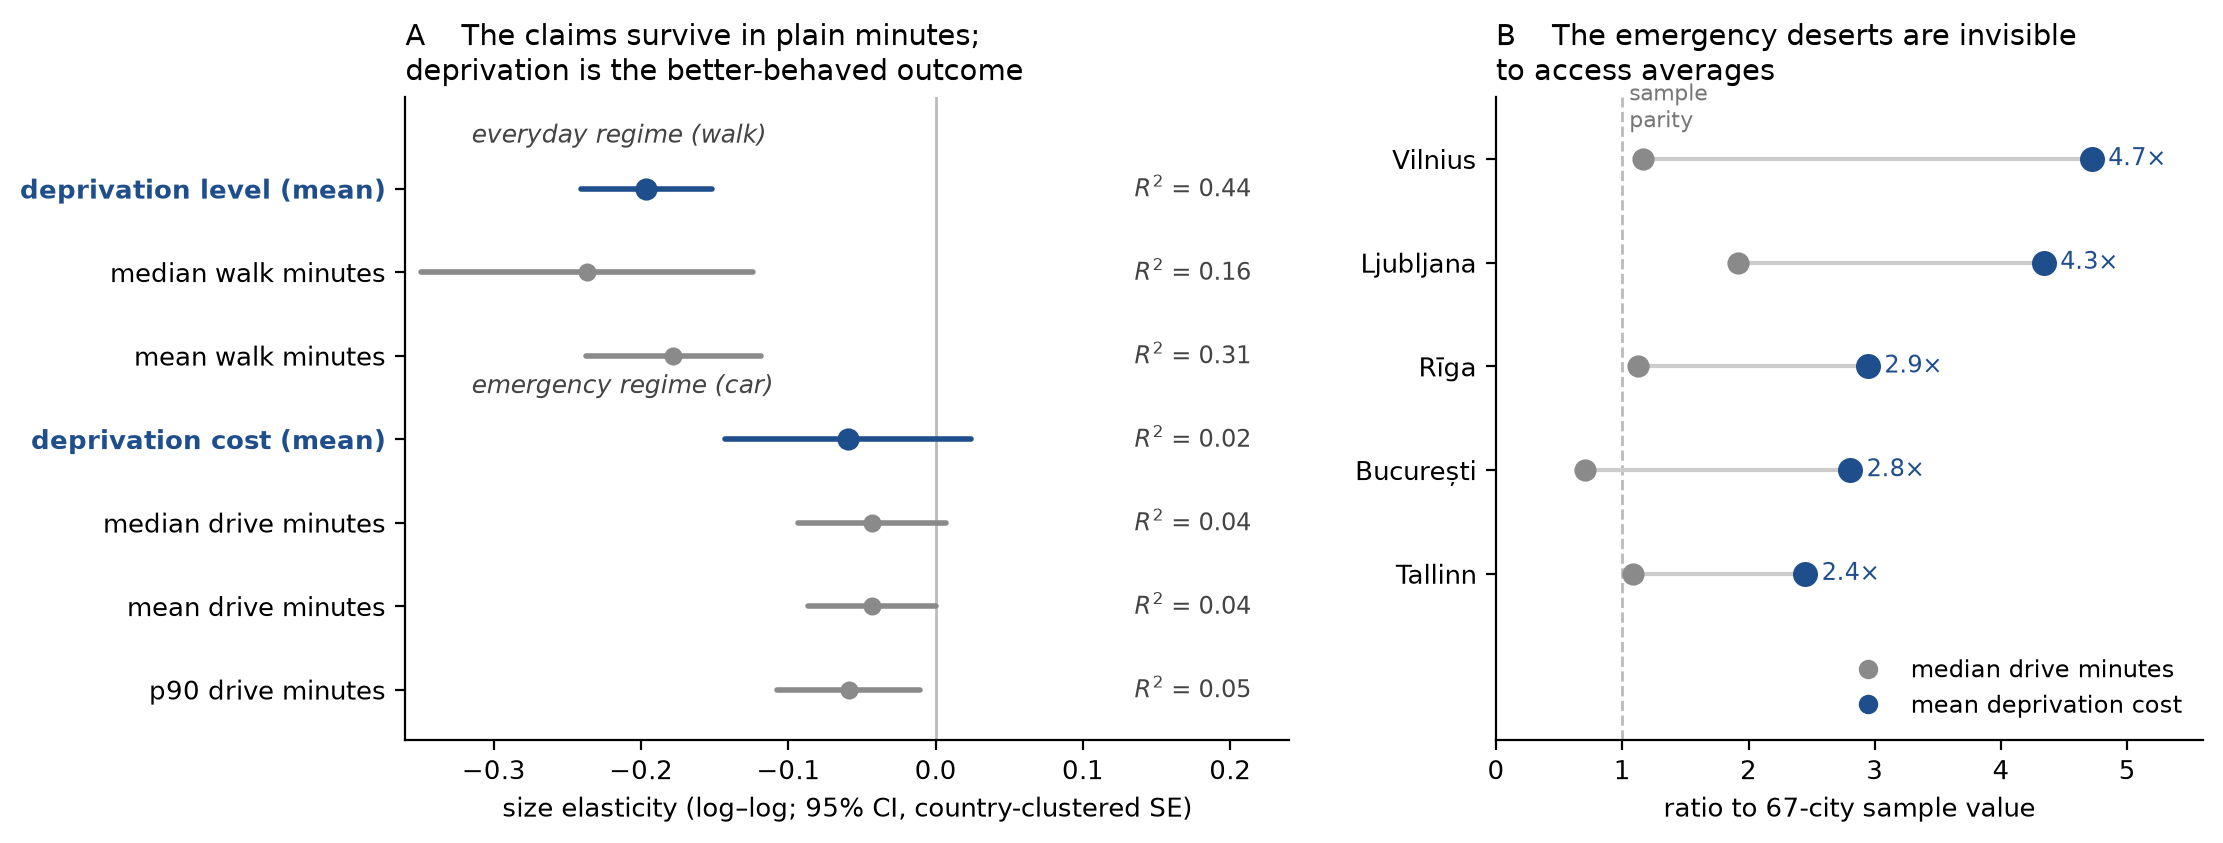
\includegraphics[width=\textwidth]{dep_vs_access.png}
\caption{Deprivation against pure access. (A) Size elasticities of
deprivation-based (blue) and minutes-based (grey) outcomes per regime
(points: estimates; bars: 95\,\% CIs on country-clustered SEs; annotations:
$R^2$). The everyday gradient and the emergency non-gradient are present
in both families; the deprivation outcomes are the better-behaved ones.
(B) The five emergency-desert capitals: ratio to the 67-city sample value
under the access average (median drive minutes, grey) and under mean
emergency deprivation cost (blue). All five sit near or below parity by
access and at 2.45--4.72 times the sample by deprivation. Sources:
\texttt{deprivation\_vs\_access.csv},
\texttt{desert\_access\_contrast.csv}.}
\label{fig:depvsaccess}
\end{figure}

\begin{table}[t]
\centering
\caption{The five emergency-desert capitals: access averages against
deprivation. Median drive time to the nearest emergency facility and its
ratio to the 67-city sample median (12 min) against mean emergency
deprivation cost (multiples of \gref{}) and its ratio to the sample value
(1.14). Source: \texttt{desert\_access\_contrast.csv}.}
\label{tab:deserts}
\small
\begin{tabular}{@{}lcrrrr@{}}
\toprule
City & Country & Median time (min) & Time ratio & Mean cost & Cost ratio \\
\midrule
Vilnius        & LT & 14.0 & 1.17 & 5.39 & 4.72 \\
Ljubljana      & SI & 23.0 & 1.92 & 4.96 & 4.34 \\
R\={\i}ga      & LV & 13.5 & 1.13 & 3.37 & 2.95 \\
Bucure\c{s}ti  & RO &  8.5 & 0.71 & 3.21 & 2.81 \\
Tallinn        & EE & 13.0 & 1.08 & 2.80 & 2.45 \\
\bottomrule
\end{tabular}
\end{table}

% ==========================================================================
\section{Discussion}\label{sec:discussion}
% ==========================================================================

\subsection{How robust is the deprivation layer itself?}\label{sec:robust}

A paper whose contribution is a measurement layer must expect that layer
to be attacked first, and the answer has two halves that both need
stating. What is varied is drawn in Fig.~\ref{fig:curves}: the Layer-1
curvature grid ($k \in \{0.1, 0.2, 0.3\}$ per minute $\times$
$t_0 \in \{10, 15, 20\}$ minutes for the everyday logistic;
$\lambda \in \{1.4, 1.8, 2.2\}$ for the emergency Box-Cox) and the
Layer-2 form swaps calibrated to the same domain anchors (a concave
Box-Cox everyday level; exponential and bounded survival-based emergency
escalations), all against the linear loss of a pure-access average.

How far the results move is in Table~\ref{tab:envelopes}. Levels are not
robust, and are not meant to be: curvature alone moves a typical city's
everyday Gini by 0.24 Gini points (median envelope width across the 67
cities), which is exactly why the calibration carries information and why
every slope claim is defended by the specification curve rather than by
one parameterisation. Ranks and classes are robust: the same curvature
grid moves the compounding share by 1.4 percentage points at the median,
the form swaps by 0.9, against 29.8 for the ``how high is high''
threshold. City-level Gini orderings survive with two scoped exceptions:
rank agreement with the baseline stays at $\rho \geq 0.90$ over the
curvature grid and the everyday form swap, while both emergency
escalation swaps reorder the emergency-Gini ranking (exponential
$\rho = 0.19$; bounded survival $\rho = 0.49$) precisely because each
changes what that Gini measures, a change of measurand reported as such
rather than noise.

The wider inventory reads as one block. Deprivation-variant flip cells,
the population whose typology class changes under any deprivation
parameterisation, average 18.1\,\% of city population (range
5.2--53.0\,\%), with the HH class share moving 2.1 percentage points on
average and 6.1 at most. The clustering survives its own feature-set
choice (main partition ARI 1.00, peeled 0.97 with benchmark shares
included). The routing-engine cross-check bounds the engine's leverage:
switching engines moves travel-time levels by 34--314\,\% and flips the
class of roughly 24\,\% of population per city, while aggregate class
shares move at most 0.7 percentage points; per-cell map readings are
therefore never findings, aggregate shares are. OSM completeness was
benchmarked against national registries where available (Germany:
pharmacies 0.976, hospitals 1.24) and the external INKAR benchmark
passed. Fig.~S1 assembles the architecture in one view. The reading
discipline it supports ran through the whole paper: rank-based results
are near-invariant to the deprivation parameterisation, and level and
inequality results are where the calibration carries the information.

\begin{table}[t]
\centering
\caption{Sensitivity envelopes of the deprivation layer: median min--max
envelope width across the 67 cities, per sweep axis and target. Curvature
moves the Ginis (the calibration carries information); no axis of the
calibration moves the compounding share materially compared with the
``how high is high'' threshold, which dominates by a factor of about 21.
The form-swap emergency-Gini envelope (0.649) spans the three
beyond-cut-off escalation hypotheses and is a boundary-of-validity
statement, reported with H2's conditionality in
Section~\ref{sec:inequality}. Source:
\texttt{deprivation\_sensitivity\_summary.csv}.}
\label{tab:envelopes}
\small
\begin{tabular}{@{}lrrr@{}}
\toprule
Sweep axis & Everyday Gini & Emergency Gini & HH share \\
\midrule
Curvature (Layer 1)            & 0.244 & 0.170 & 0.014 \\
Form swap (Layer 2)            & 0.035 & 0.649 & 0.009 \\
``How high is high'' threshold & --    & --    & 0.298 \\
\bottomrule
\end{tabular}
\end{table}

\subsection{What the results change for theory}\label{sec:theory}

\paragraph{1. Urban scaling: returns to scale in welfare are
regime-specific.}
Scaling theory's power of generalisation rests on exponents that hold
across cities, systems and quantities, with infrastructure in a single
sublinear universality class \citep{bettencourt2007growth}; its recent
refinements condition exponents on national context
\citep{musso2026cities}. Our results add a different kind of condition:
the exponent depends on the welfare regime of the service class, within
one urban system and one harmonised measurement. Everyday welfare scales
($-0.196$, explaining 44\,\% of cross-city variance); emergency welfare
does not (bounded within $\pm 0.13$); and the two slopes differ within
cities (\pw{0.002}). A single infrastructure exponent is therefore not a
sufficient statistic for what city size does to service welfare, and
theories that read agglomeration as generalised provisioning gain
overstate what growth delivers. The inequality result cuts deeper:
everyday welfare inequality \emph{rises} with size under every
parameterisation tested, so the same agglomeration that lowers mean
everyday deprivation widens its spread. Scaling theory has largely
concerned means; these results argue that the scaling of within-city
distributions, and specifically of welfare-weighted distributions, is
where the next generation of urban scaling laws has to live.

\paragraph{2. Accessibility and urbanism: impedance must be
welfare-anchored.}
For the accessibility literature the contribution is a measurement
theorem demonstrated at continental scale. Where results are rank-based,
minutes and deprivation agree almost perfectly ($r \geq 0.965$ between
the Gini families), which certifies the field's rank-level findings.
Where results concern levels, inequality magnitudes or tails, uniform
minutes are not a welfare measure, and the divergence is not noise: the
desert capitals sit at 0.71--1.92 times the sample by access and at
2.45--4.72 times it by deprivation (Table~\ref{tab:deserts}), and the
choice of measure decides whether an emergency-side size story exists at
all. The 15-minute-city doctrine
\citep{moreno2021fifteenminute,papadopoulos2023compliance} emerges
recast: its threshold anchors the everyday regime well, and precisely
because that regime saturates, a proximity doctrine is an
everyday-services doctrine, silent about the escalating-cost regime and
about the compounded populations where both fail. The coverage grades
(covered, partial desert, desert) offer the tail-sensitive screening
object that averages cannot supply, and the framework as a whole (forms
transferred from an estimated literature, curvature calibrated to
domain anchors, robustness of ranks separated from meaning of levels)
travels to any domain that possesses anchors of comparable strength.

\paragraph{3. Resilience: two capabilities, coupled where it hurts.}
Resilience theory has moved toward defining resilience as equitable
access to essential services \citep{logan2020reframing,meerow2016defining}
and has documented that access equality and network resilience reinforce
each other \citep{fan2022equality}, while empirical work shows everyday
vulnerability failing to predict crisis capability
\citep{sirenko2026heatwaves}. Our two-regime measurement gives that
distinction quantitative form across an urban system: the everyday and
emergency surfaces are distinct objects with different scaling laws and
different geographies, so a city's resilience portfolio cannot be read
from either alone. The compounding result identifies the pathological
case the coupled-systems argument predicts: the same residents in the
periphery of both systems, above statistical independence in 66 of 67
cities, strongest exactly where emergency inequality is highest
(Central-Eastern Europe). Compounding intensity, with its fixed anchors
under independence and perfect coupling, is offered as a general-purpose
measure of that coupling for any pair of capability surfaces.

\subsection{Implications for planning and policy}\label{sec:policy}

The practical reading is short, because the two regimes point at two
different jurisdictions. Everyday inequality is a big-city problem: it
rises with size under every parameterisation, so the cities gaining
everyday access on average are the ones whose internal spread widens,
and intra-urban service planning is the lever. Emergency deprivation is
a national coverage problem: it is set by coverage grade rather than
size, differs by country and macro-region, and its extreme cases are
five capital cities whose peripheries no municipal instrument can serve
alone. The severity ordering gives national emergency-system planners a
screening variable that access averages do not provide. And the
consistent carriers of compounded deprivation at the European level are
families with children, in 88\,\% of the cities studied, which makes
school- and family-anchored service planning a compounding remedy rather
than a sectoral one.

\subsection{Limitations}\label{sec:limitations}

Every size gradient is cross-sectional; the space-for-time reading was
flagged once and applies throughout. The analysis covers walking for
everyday services and driving for emergency care; public transit is
deliberately out of scope, and the everyday regime is walk-only by
design. Census strata arrive on a 1\,km grid broadcast to the 100\,m
analysis grid, so they are neighbourhood attributes; employment is
unreported in the census grid for Germany and France, so no harmonised
SES slope exists there by design. Per-cell typology classes carry a
roughly 24\,\% routing-engine flip share and are read only as spatial
patterns. Population shares beyond fixed time thresholds contain the
finite-fill constant assigned to service-deprived cells and are
footnoted wherever used. The emergency-side external benchmark (INKAR)
is unavailable, and the German registry counts carry a
verify-before-publication flag.

Two OSM completeness specifics deserve statement rather than smoothing.
Mapped GP density varies about 12-fold across countries in a way that
reflects tagging conventions rather than health systems: the median FUA
has 10.8 mapped GPs per 100k inhabitants, yet the country medians are
2.1 in Sweden, 2.3 in Portugal, 2.6 in Finland and 3.5 in Italy against
24.5 across the West, because primary care there sits in health centres
OSM tags differently. Everyday deprivation levels are correspondingly
overstated in those countries, so cross-country everyday \emph{level}
comparisons are not supported (one plausible reason the everyday-Gini
regional contrast fails country-level testing). The size gradients are
unaffected: mapped GP density is uncorrelated with city size (log-log
slope $+0.09$, country-clustered $p = 0.29$), and every scaling claim is
country-clustered. Separately, eight cities have only one of the two
emergency services mapped (Athina, Br\u{a}ila, Helsinki, Lahti,
Norrk\"oping, Szeged, Talavera de la Reina, \v{Z}ilina); the composite
renormalises weights over the services present, their median mean
emergency cost is 0.197 against 0.169 for the rest, the expected
direction at a modest size, and none of them is in the desert group, so
no headline turns on it. Table~\ref{tab:si-cities} reports the count per
city.

% ==========================================================================
\section{Materials and Methods}\label{sec:methods}
% ==========================================================================

\paragraph{Design and sample.}
Cross-sectional multi-city design with one harmonised city definition
(Eurostat/OECD functional urban areas) and trajectories read from the
cross-sectional size gradient
\citep{musso2026cities,bettencourt2007growth}; no longitudinal component
exists, and all outputs are labelled space-for-time. The sample is a
stratified draw over 4 macro-regions $\times$ 4 population strata: 67
FUAs, 24 countries, 113.9 million residents, 101{,}050 to 12.9 million
inhabitants (Table~\ref{tab:sample}; Table~\ref{tab:si-cities}).

\paragraph{Grid, facilities, routing.}
The analysis grid is the GHS-POP 100\,m population grid
\citep{schiavina2023ghspop}, cells clipped to each FUA. Facilities come
from OpenStreetMap via Overpass queries with expiry-refreshed
extractions; Table~\ref{tab:services} summarises the routed facility
sets. Travel times are computed with the R5 routing engine via r5py
\citep{fink2022r5py} over the OSM street network: walking for the
everyday regime, driving for the emergency regime, with emergency
matrices reverse-routed (station-to-cell, the substantively correct
direction for ambulance response; measured car asymmetry median 1
minute). A friction-surface engine \citep{weiss2020healthcare} is
retained as a declared sensitivity variant after a two-city cross-check
showed city-specific, uncorrectable level bias (E.1).

\begin{table}[t]
\centering
\caption{Facilities routed to (medians across the 67 FUAs) and
population-weighted median travel times to the nearest facilities of
each service. Everyday services are reached on foot, emergency services
by car. Source: \texttt{accessibility\_by\_service\_pooled.csv}.}
\label{tab:services}
\small
\begin{tabular}{@{}llrr@{}}
\toprule
Regime & Service & Facilities per FUA & Median time (min) \\
\midrule
Everyday  & general practitioner   & 93  & 7.9 \\
Everyday  & pharmacy               & 228 & 4.9 \\
Everyday  & supermarket            & 325 & 4.7 \\
Everyday  & school                 & 409 & 4.4 \\
Everyday  & green space            & 636 & 3.8 \\
Emergency & emergency department   & 6   & 12.0 \\
Emergency & ambulance station      & 6   & 12.0 \\
\bottomrule
\end{tabular}
\end{table}

\paragraph{Everyday deprivation (a level).}
Per service, travel time is congestion-adjusted by a two-step floating
catchment area (2SFCA) factor \citep{luo2003measures,luo2009enhanced}:
facilities serving many people relative to capacity inflate the
effective time of their users. A soft-minimum over reachable facilities
then rewards substitutability (several similar options count as slightly
closer than the nearest alone). The effective time passes through a
logistic deprivation level function \citep{wang2017deprivation} with
ceiling 1, inflection $t_0 = 15$ minutes (the 15-minute-city threshold
\citep{moreno2021fifteenminute}) and steepness $k = 0.2$ per minute; the
city surface is the weighted mean over the five service categories
(school and green-space sub-types weigh 0.5 each). Cells with no network
path to any facility are masked; routable cells beyond a service's
cutoff receive a large finite time so they stay on the map at
near-maximal deprivation.

\paragraph{Emergency deprivation (a cost).}
The emergency surface applies a convex Box-Cox deprivation cost function
\citep{cantillo2018discrete,delgadolindeman2019ambulance} with
$\lambda = 1.8$ (transferred; solving $\lambda$ from the anchors gives
1.89--1.95, inside the sensitivity sweep) to the drive time to the
nearest emergency facility. The anchors are the EMS response benchmarks:
cost negligible below the 3--4 minute ideal
\citep{pons2005response,vo2020vulnerable}, about a third of the
benchmark cost at the 8-minute urban standard (contested: no survival
effect for most patients in \citep{pons2005response}, supported in
\citep{blanchard2012response}; attributed via \citep{khan2026melbourne},
whose WHO 2020 reference is an unpinnable URL), and 1 at the 15-minute
upper target \citep{peleg2004ems,khan2026melbourne}; convexity is
supported independently by distance-mortality evidence
\citep{nicholl2007distance}. The 8-minute mark cannot carry a half-max
anchor: convexity caps $g(8)/g(15)$ at 0.427 given $g(4)/g(15) = 0.10$,
so the two regimes' anchor structures are genuinely different. All costs
are reported in multiples of $\gref$. Free-flow civilian drive times
anchor the cost scale and are not literal response-time predictions
(dispatch and turnout are unmodelled; lights-and-siren travel is faster
than civilian flow; free-flow understates congested cores, which is
conservative for the periphery findings).

\paragraph{Cross-regime standardisation.}
The everyday level and the emergency cost are on incomparable scales by
design. Only unit-invariant statistics cross regimes: elasticities,
Ginis (mean-normalised, the same move as comparing an income Gini with a
wealth Gini) and rank-based measures. The co-location typology is built
on population-weighted mid-rank percentile surfaces; at the median split
the 2$\times$2 class table has one free number, the HH share, and
statistical independence corresponds to HH $= 25\,\%$. The continuous
compounding intensity is the population-weighted mean of the smaller of
the two percentile ranks (1/3 independence, 1/2 perfect coupling, 1/4
perfect divergence). The divergence gap (emergency Gini minus everyday
Gini) is the one cross-regime subtraction, a difference of dimensionless
indices, form-dependent, and never a standalone headline.

\paragraph{Equity strata.}
Census-2021 1\,km strata (broad age groups) are broadcast to the grid
and pooled across cities against covered-cell references (cells where
the stratum's variable is published); national fine-grid strata (rent,
tenure) are per-city depth and never pooled. Inequality within strata
uses the concentration index \citep{wagstaff1991measurement}.

\paragraph{Cross-city inference.}
Cities nest in 24 countries, so scaling regressions report
country-clustered standard errors with wild cluster bootstrap p-values
(null imposed) \citep{cameron2008bootstrap,mackinnon2023cluster};
regional contrasts are tested by permuting whole countries across
macro-regions, with a country-random-intercept mixed model as
triangulation; city-level ANOVA p-values are anti-conservative for such
questions and are never cited as evidence. The emergency null is bounded
by TOST equivalence tests \citep{lakens2017equivalence}; slope
robustness uses a specification curve over all 14 deprivation
parameterisations \citep{simonsohn2020specification}; clustering
diagnostics report silhouette \citep{rousseeuw1987silhouettes},
bootstrap and cross-partition adjusted Rand indices
\citep{hubert1985comparing} and a Gaussian silhouette null. Every
headline elasticity carries leave-one-out, Cook's-distance, Huber and
median-regression diagnostics.

\paragraph{Robustness harness.}
A structured (non-probabilistic) sweep recomputes rank-based targets
over a defensible envelope: Layer 1 varies curvature within fixed forms;
Layer 2 swaps the forms while pinning the same anchors (concave Box-Cox
everyday; exponential and bounded survival-based emergency escalations);
Layer 3 sweeps the accessibility model (soft-min $\kappa$, congestion
exponent $\gamma$, bandwidth, $k$-nearest, mode set, unreachable
policy); a threshold axis sweeps the typology cut. Results are reported
as rank agreement, class-share envelopes, flip-cell shares and the
specification curve (Section~\ref{sec:robust}; Fig.~S1).

\paragraph{Reproducibility.}
The pipeline is config-driven with provenance sidecars on every derived
matrix; all tables and figures in this paper trace to the persisted
67-city state (every quoted number is checked against its source table
by an automated audit of 133 checks run in CI). Code, configuration and
the full result tables are available in the study repository.

\paragraph{Data availability.}
Population grid: GHS-POP R2023A \citep{schiavina2023ghspop}. Facilities
and street networks: OpenStreetMap. Census strata: Eurostat Census 2021
grid. Per-city and cross-city result tables, per-city maps and
sensitivity sweeps are persisted on the study repository's results
branch.

% ==========================================================================
\bibliographystyle{unsrtnat}
\bibliography{references}

% ==========================================================================
\clearpage
\appendix
\renewcommand{\thesection}{S\arabic{section}}
\renewcommand{\thetable}{S\arabic{table}}
\renewcommand{\thefigure}{S\arabic{figure}}
\setcounter{section}{0}
\setcounter{table}{0}
\setcounter{figure}{0}

\begin{center}
{\LARGE Supplementary Information}\\[6pt]
{\large The two geographies of urban deprivation}
\end{center}

% --------------------------------------------------------------------------
\section{The robustness architecture in one view}\label{si:architecture}

\begin{figure}[h]
\centering
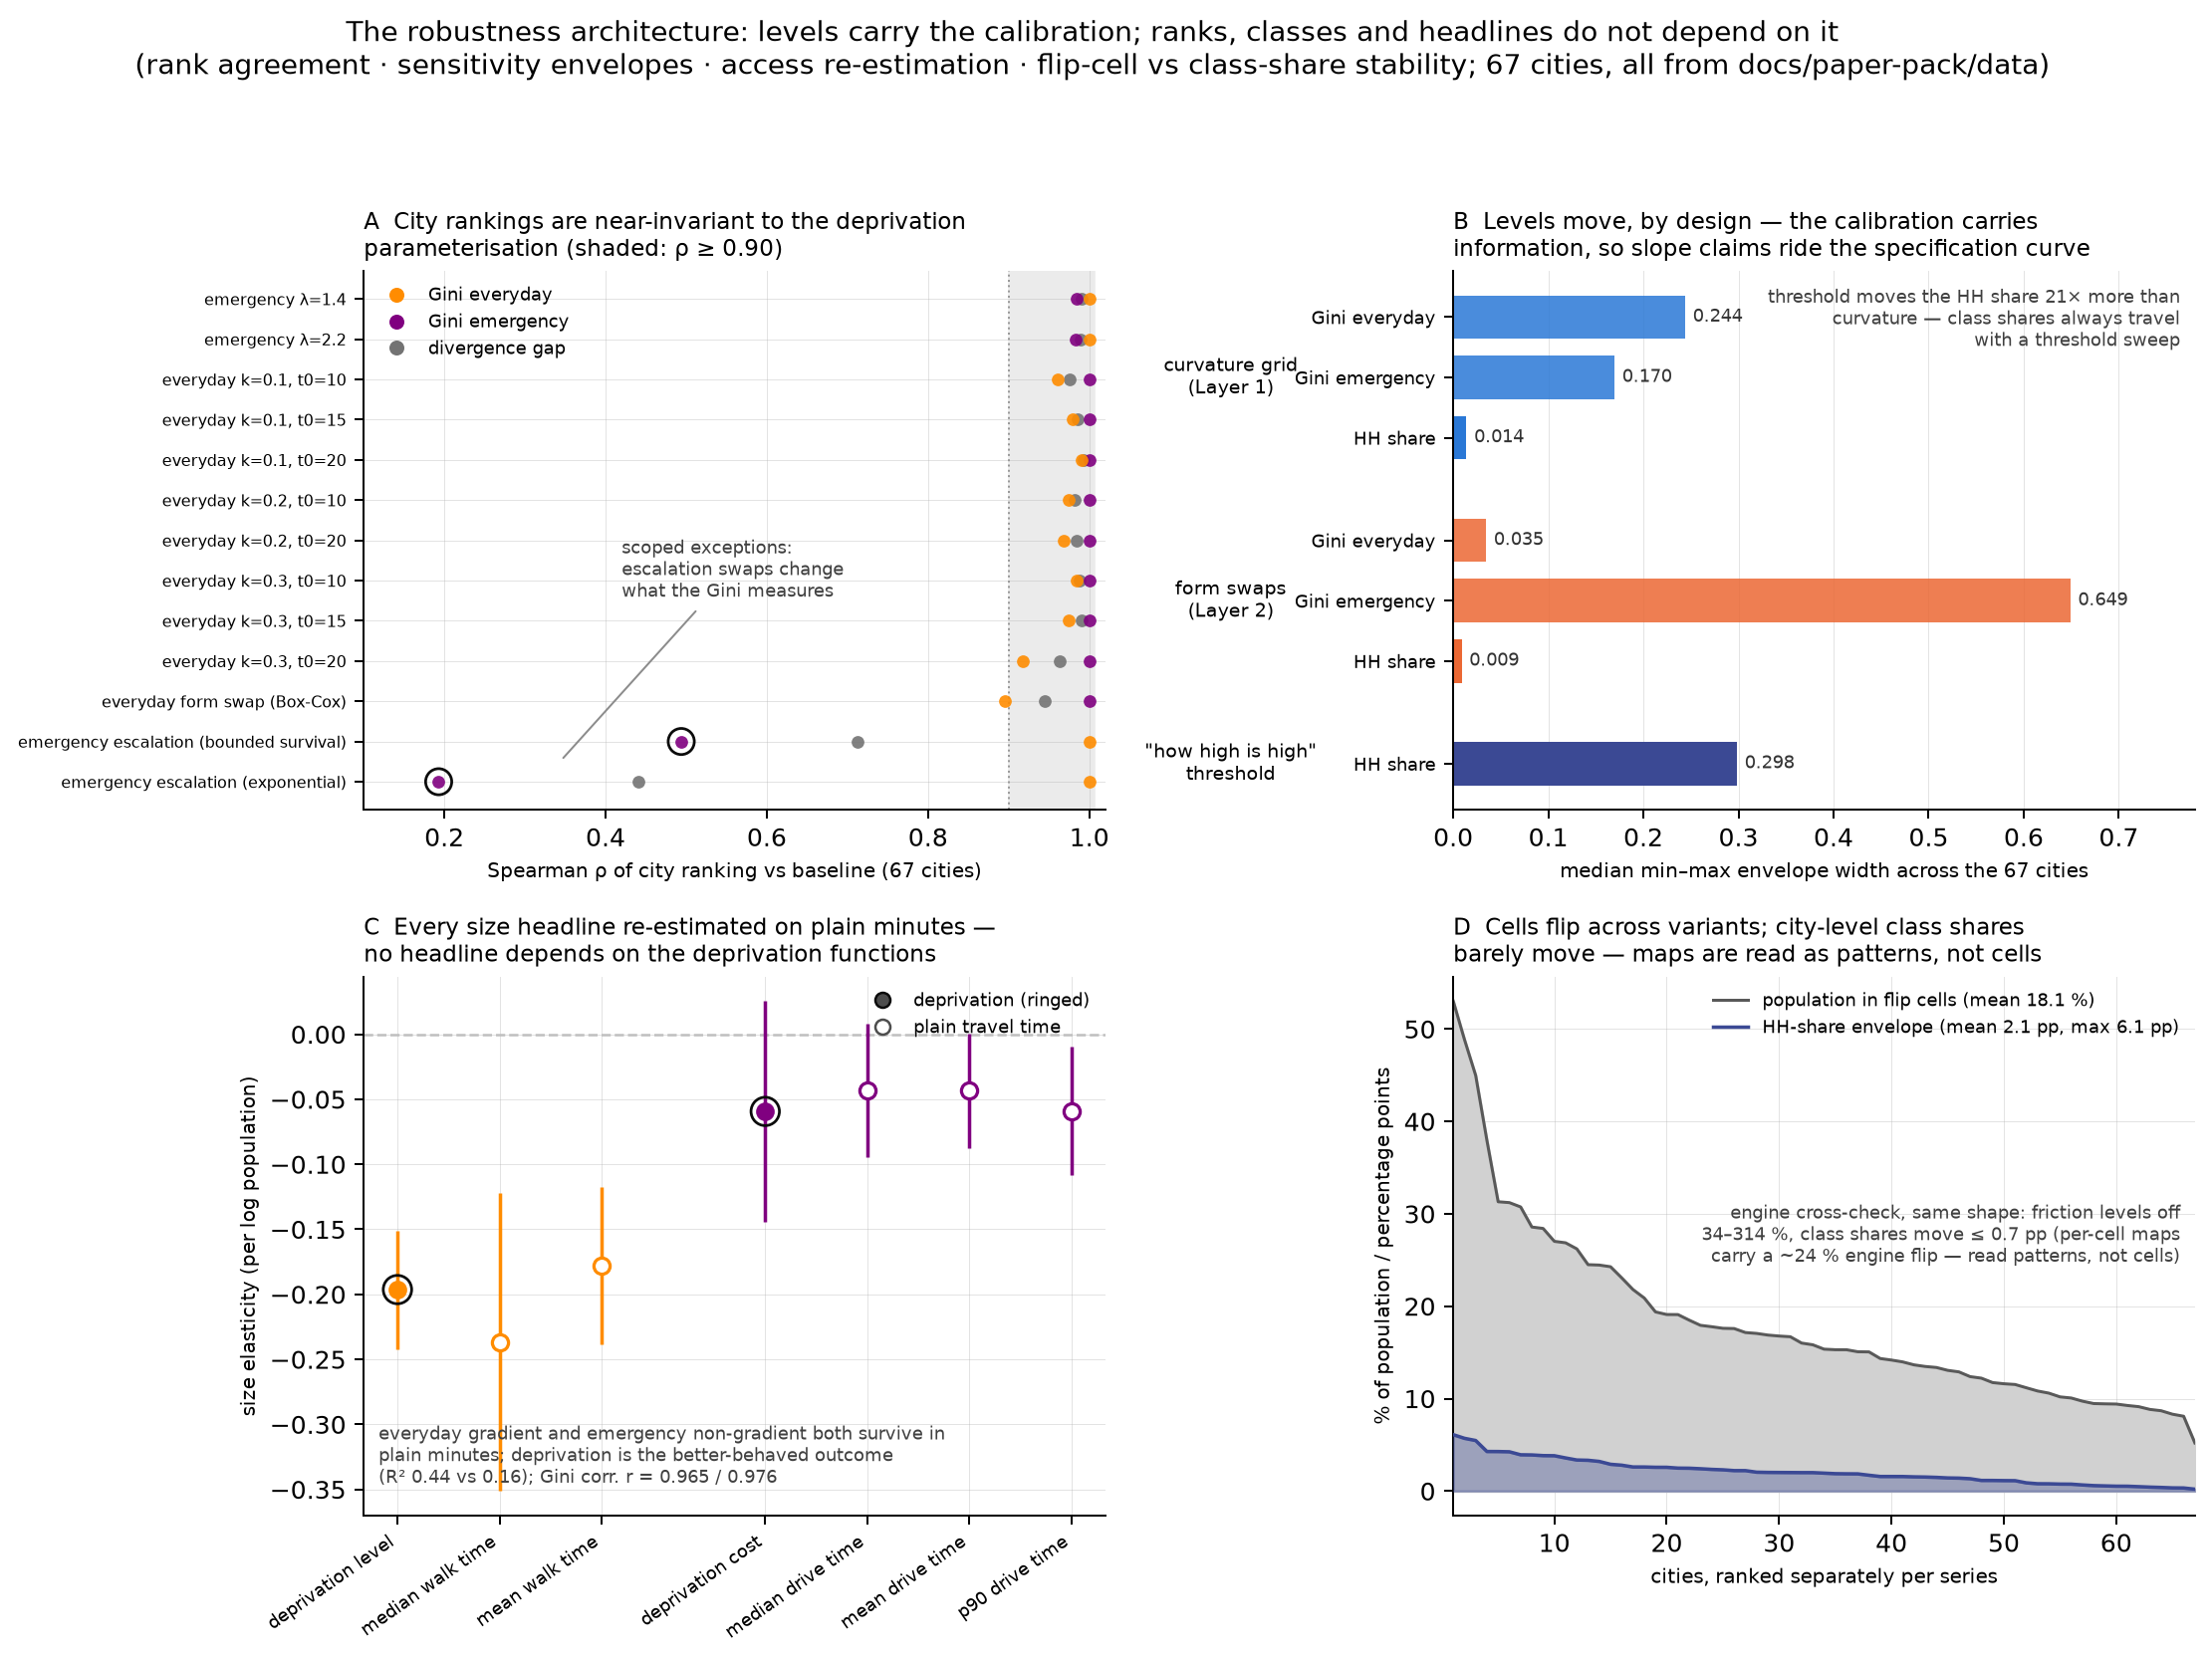
\includegraphics[width=\textwidth]{robustness_architecture.png}
\caption{The robustness architecture (contribution claim 5). One view of
the checks defending the results: rank agreement of city orderings across
deprivation variants (min $\rho = 0.90$ over the curvature grid and
everyday form swap; the two emergency escalation swaps are scoped
exceptions that change the measurand, $\rho = 0.19$ exponential, 0.49
bounded survival); sensitivity envelope widths per axis
(Table~\ref{tab:envelopes}); access-based re-estimation of every headline
(Table~\ref{tab:si-depvsaccess}); and flip-cell against class-share
stability (population-weighted flip share 18.1\,\% on average,
5.2--53.0\,\% across cities, against HH class-share movement of 2.1 pp
average, 6.1 pp maximum), with the routing-engine cross-check quoted
alongside (engine flip $\approx 24\,\%$, aggregate class shares
$\leq 0.7$ pp).}
\label{fig:si-architecture}
\end{figure}

Rank-based results are near-invariant to the deprivation
parameterisation; level and inequality results move with the
calibration, which is where the calibration carries information. The
flagged exceptions are exactly the two emergency escalation swaps, each
of which changes what the emergency Gini measures (an extreme-tail-depth
ordering under exponential escalation; a benchmark-window inequality
ordering under the bounded survival curve), and they are reported as
changes of measurand.

% --------------------------------------------------------------------------
\section{Size gradient of the divergence measures}\label{si:sizegradient}

\begin{figure}[h]
\centering

\includegraphics[width=.85\textwidth]{size_gradient.png}
\caption{The divergence gap (emergency Gini minus everyday Gini) against
$\log_{10}$ FUA population, coloured by macro-region with the
emergency-desert capitals outlined. The gap falls weakly with size
($-0.066$ per decade of population, $p = 0.012$, $R^2 = 0.06$). Size is
a poor predictor of where the two regimes diverge; the structure is
regional and coverage-graded (main text Section~2.3).}
\label{fig:si-sizegradient}
\end{figure}

The companion gradients are weaker still: the coupling $\rho$
($p = 0.14$) and the compounding share ($p = 0.06$) show no significant
size gradient (\texttt{size\_gradient.csv}).

% --------------------------------------------------------------------------
\section{Deprivation vs access: exact values}\label{si:depvsaccess}

\begin{table}[h]
\centering
\caption{Size elasticities of deprivation-based and minutes-based
outcomes (log-log, country-clustered SEs, 67 cities; cross-sectional
space-for-time), plotted in main-text Fig.~\ref{fig:depvsaccess}A. The
everyday p90 is not regressed: above the walk cutoff the everyday
composite time behaves as a count of unmet service categories rather
than a travel time. Source: \texttt{deprivation\_vs\_access.csv}.}
\label{tab:si-depvsaccess}
\small
\begin{tabular}{@{}llrrr@{}}
\toprule
Regime & Outcome & Elasticity & $p$ & $R^2$ \\
\midrule
Everyday  & mean deprivation level      & $-0.196$ & $<0.001$ & 0.44 \\
Everyday  & median walk time            & $-0.237$ & $<0.001$ & 0.16 \\
Everyday  & mean walk time              & $-0.178$ & $<0.001$ & 0.31 \\
\addlinespace
Emergency & mean deprivation cost       & $-0.059$ & 0.16     & 0.02 \\
Emergency & median drive time           & $-0.043$ & 0.09     & 0.04 \\
Emergency & mean drive time             & $-0.043$ & 0.05     & 0.04 \\
Emergency & p90 drive time              & $-0.059$ & 0.02     & 0.05 \\
\bottomrule
\end{tabular}
\end{table}

% --------------------------------------------------------------------------
\section{Validation exercises}\label{si:validation}

\paragraph{E.1 Routing-engine cross-check.} Re-running full cities under
the friction-surface engine against the R5 baseline (Hamburg, K\"oln)
shows travel-time levels understated by 34--314\,\% with city-specific
Gini bias (emergency Gini $-30$\,\% in Hamburg, $-18.5$\,\% in K\"oln),
which demoted friction to sensitivity variant. Aggregate typology class
shares move $\leq 0.7$ pp and the divergence $\rho$ by $\leq 11\,\%$,
while roughly 24\,\% of population flips per-cell class; hence per-cell
map readings are never findings.

\paragraph{E.2 OSM completeness.} Country-level benchmark against
national registries where available: Germany, pharmacies ratio 0.976,
hospitals 1.24 (the hospital ratio carries a verify-before-publication
flag on the registry side). The per-city facility counts
(\path{accessibility_by_service_cities.csv}) provide the cross-country
completeness picture the single-country registry benchmark cannot, and
surface the GP tagging artefact discussed in the limitations.

\paragraph{E.3 External benchmark.} The German INKAR accessibility
indicators reproduce the study's German pharmacy and supermarket access
patterns (passed); no comparable emergency-side benchmark is available.

\paragraph{E.4 Resolution and E.5 face validation.} Quantile-curve
comparisons of regime times under both engines and per-anchor-city face
validation documents are maintained in the study repository.

\paragraph{Re-anchor verification.} The emergency reporting anchor moved
from $g(45)$ to $\gref$ in August 2026. For the three cities re-seeded
from stored artifacts the verification is exact: every rank-based
indicator is identical to machine precision (max $|\Delta| \approx
10^{-16}$) and the level ratio equals $g(45)/g(15) = 6.7307$ to
$10^{-15}$; the other 64 cities were byte-identical between the two
runs.

% --------------------------------------------------------------------------
\section{Indicator glossary}\label{si:glossary}

\begin{table}[h]
\centering
\caption{Compact glossary of the indicators used in this paper.}
\label{tab:si-glossary}
\small
\begin{tabular}{@{}p{0.32\textwidth}p{0.62\textwidth}@{}}
\toprule
Term & Meaning \\
\midrule
FUA & Functional urban area (Eurostat/OECD): city plus commuting zone; the unit ``city''. \\
Everyday regime & Five walkable service categories (GP, pharmacy, supermarket, school, green space); deprivation is a bounded \emph{level} in $[0,1]$. \\
Emergency regime & ED hospital and ambulance station, reached by car; deprivation is an unbounded convex \emph{cost} in multiples of \gref{}. \\
$\bar D_{\mathrm{ev}}$, $\bar C_{\mathrm{em}}$ & Population-weighted mean deprivation per regime; scales are incomparable across regimes. \\
$G_{\mathrm{ev}}$, $G_{\mathrm{em}}$ & Population-weighted within-city Gini of each surface. \\
Divergence gap & $G_{\mathrm{em}} - G_{\mathrm{ev}}$; positive = emergency-side inequality problem. \\
$\rho$ & Spearman correlation of the two population-weighted percentile surfaces. \\
LL/LH/HL/HH & Median-split co-location classes; HH = compounding. At the median split the table has one free number (HH); independence = 25\,\%. \\
Compounding intensity & Population-weighted mean of $\min$(everyday pct, emergency pct); 1/3 independence, 1/2 coupled, 1/4 divergent. \\
Coverage grade & Severity ordering from the two clustering passes: covered / partial desert / desert. \\
Elasticity & Slope of log outcome on log population (space-for-time). \\
Wild cluster bootstrap & Country-clustered resampling giving reliable p-values with 24 clusters; the citable p for scaling claims. \\
$p_{\mathrm{perm}}$ & Permutation p-value reshuffling whole countries across macro-regions; the primary regional test. \\
TOST & Two one-sided equivalence tests; positive evidence a slope lies within a bound. \\
Specification curve & Headline regression re-estimated under every deprivation parameterisation. \\
Flip cells & Cells whose typology class changes under any deprivation variant. \\
\bottomrule
\end{tabular}
\end{table}

\clearpage

% --------------------------------------------------------------------------
\section{Per-city table}\label{si:cities}

% AUTOGENERATED by make_includes.py from
% docs/paper-pack/data/cities_descriptives.csv -- do not edit by hand.
\begin{footnotesize}
\setlength{\tabcolsep}{3.5pt}
\begin{longtable}{@{}llllr c rrrrrr@{}}
\caption{The 67 functional urban areas, largest first. Grade: emergency-periphery
coverage grade (Section~\ref{sec:coverage}); $n_{\mathrm{em}}$: number of mapped
emergency services (2 = both ED hospital and ambulance station);
$\bar D_{\mathrm{ev}}$: population-weighted mean everyday deprivation level (0--1);
$\bar C_{\mathrm{em}}$: mean emergency deprivation cost in multiples of the 15-min
benchmark cost $g(15)$; $G$: population-weighted Gini per regime; $\rho$: Spearman
coupling of the two percentile surfaces; HH: compounding population share at the
median split.}\label{tab:si-cities}\\
\toprule
City & CC & Region & Population & Grade & $n_{\mathrm{em}}$ &
$\bar D_{\mathrm{ev}}$ & $\bar C_{\mathrm{em}}$ &
$G_{\mathrm{ev}}$ & $G_{\mathrm{em}}$ & $\rho$ & HH \\
\midrule
\endfirsthead
\multicolumn{12}{l}{\emph{Table \ref{tab:si-cities} continued}}\\
\toprule
City & CC & Region & Population & Grade & $n_{\mathrm{em}}$ &
$\bar D_{\mathrm{ev}}$ & $\bar C_{\mathrm{em}}$ &
$G_{\mathrm{ev}}$ & $G_{\mathrm{em}}$ & $\rho$ & HH \\
\midrule
\endhead
\bottomrule
\endlastfoot
Paris & FR & West & 12,886,280 & covered & 2 & 0.135 & 0.73 & 0.625 & 0.497 & 0.50 & 0.334 \\
Madrid & ES & South & 7,601,394 & covered & 2 & 0.191 & 0.62 & 0.533 & 0.439 & 0.39 & 0.316 \\
Barcelona & ES & South & 5,945,709 & covered & 2 & 0.175 & 0.84 & 0.545 & 0.418 & 0.36 & 0.309 \\
Milano & IT & South & 5,030,024 & covered & 2 & 0.183 & 0.61 & 0.400 & 0.400 & 0.37 & 0.319 \\
Berlin & DE & West & 4,875,655 & covered & 2 & 0.158 & 0.62 & 0.558 & 0.438 & 0.38 & 0.317 \\
Roma & IT & South & 4,432,845 & covered & 2 & 0.287 & 1.14 & 0.424 & 0.503 & 0.48 & 0.342 \\
Athina & EL & South & 3,522,264 & covered & 1 & 0.103 & 0.73 & 0.609 & 0.500 & 0.28 & 0.274 \\
Bruxelles & BE & West & 3,521,497 & covered & 2 & 0.182 & 1.29 & 0.583 & 0.286 & 0.40 & 0.332 \\
Napoli & IT & South & 3,457,649 & covered & 2 & 0.326 & 0.83 & 0.305 & 0.384 & 0.15 & 0.270 \\
Warszawa & PL & CEE & 3,334,987 & partial & 2 & 0.225 & 1.99 & 0.589 & 0.590 & 0.49 & 0.347 \\
Hamburg & DE & West & 3,162,607 & covered & 2 & 0.260 & 0.58 & 0.543 & 0.437 & 0.40 & 0.321 \\
Bucure{\c{s}}ti & RO & CEE & 3,140,502 & desert & 2 & 0.335 & 3.21 & 0.524 & 0.774 & 0.73 & 0.424 \\
Lisboa & PT & South & 3,132,904 & covered & 2 & 0.239 & 1.19 & 0.367 & 0.409 & 0.48 & 0.319 \\
M{\"u}nchen & DE & West & 3,054,507 & covered & 2 & 0.178 & 0.60 & 0.616 & 0.449 & 0.35 & 0.304 \\
Budapest & HU & CEE & 3,030,949 & covered & 2 & 0.183 & 1.05 & 0.538 & 0.507 & 0.48 & 0.327 \\
Amsterdam & NL & West & 2,829,893 & covered & 2 & 0.227 & 0.75 & 0.501 & 0.326 & 0.20 & 0.285 \\
Stockholm & SE & North & 2,549,795 & partial & 2 & 0.267 & 1.73 & 0.460 & 0.513 & 0.65 & 0.389 \\
K{\"o}ln & DE & West & 2,438,338 & covered & 2 & 0.204 & 0.57 & 0.520 & 0.398 & 0.36 & 0.312 \\
Praha & CZ & CEE & 2,247,160 & covered & 2 & 0.282 & 1.11 & 0.515 & 0.475 & 0.46 & 0.354 \\
K{\o{}}benhavn & DK & North & 2,180,998 & covered & 2 & 0.254 & 0.94 & 0.401 & 0.401 & 0.30 & 0.307 \\
Sofia & BG & CEE & 1,647,936 & partial & 2 & 0.285 & 1.44 & 0.511 & 0.600 & 0.73 & 0.408 \\
Helsinki & FI & North & 1,642,879 & covered & 1 & 0.379 & 1.36 & 0.341 & 0.426 & 0.26 & 0.270 \\
Oslo & NO & North & 1,550,450 & partial & 2 & 0.209 & 2.06 & 0.553 & 0.467 & 0.39 & 0.297 \\
Porto & PT & South & 1,531,690 & covered & 2 & 0.324 & 0.85 & 0.272 & 0.395 & 0.42 & 0.321 \\
Krak{\'o}w & PL & CEE & 1,350,286 & covered & 2 & 0.308 & 1.50 & 0.523 & 0.519 & 0.58 & 0.396 \\
Katowice & PL & CEE & 1,341,890 & covered & 2 & 0.168 & 1.02 & 0.489 & 0.279 & 0.10 & 0.267 \\
Zagreb & HR & CEE & 1,293,698 & partial & 2 & 0.343 & 2.07 & 0.499 & 0.583 & 0.70 & 0.395 \\
Antwerpen & BE & West & 1,219,366 & covered & 2 & 0.289 & 0.77 & 0.523 & 0.406 & 0.29 & 0.311 \\
R{\={\i}}ga & LV & CEE & 1,110,303 & desert & 2 & 0.362 & 3.37 & 0.502 & 0.682 & 0.55 & 0.374 \\
Bilbao & ES & South & 1,053,444 & covered & 2 & 0.160 & 1.06 & 0.570 & 0.433 & 0.42 & 0.324 \\
{\L{}}{\'o}d{\'z} & PL & CEE & 1,045,886 & covered & 2 & 0.255 & 1.60 & 0.534 & 0.491 & 0.33 & 0.310 \\
G{\"o}teborg & SE & North & 1,042,720 & partial & 2 & 0.427 & 2.44 & 0.335 & 0.446 & 0.31 & 0.298 \\
Vilnius & LT & CEE & 1,010,376 & desert & 2 & 0.462 & 5.39 & 0.411 & 0.739 & 0.55 & 0.358 \\
Palermo & IT & South & 1,006,055 & partial & 2 & 0.317 & 3.64 & 0.383 & 0.292 & 0.27 & 0.289 \\
Alicante & ES & South & 996,867 & covered & 2 & 0.311 & 1.80 & 0.530 & 0.277 & 0.15 & 0.269 \\
Wroc{\l{}}aw & PL & CEE & 939,076 & covered & 2 & 0.199 & 1.47 & 0.609 & 0.362 & 0.41 & 0.341 \\
Bratislava & SK & CEE & 931,613 & covered & 2 & 0.296 & 1.78 & 0.522 & 0.430 & 0.39 & 0.336 \\
Ljubljana & SI & CEE & 919,303 & desert & 2 & 0.447 & 4.96 & 0.387 & 0.481 & 0.48 & 0.341 \\
Palma de Mallorca & ES & South & 818,202 & covered & 2 & 0.251 & 1.39 & 0.503 & 0.453 & 0.14 & 0.294 \\
Brno & CZ & CEE & 745,397 & covered & 2 & 0.286 & 1.14 & 0.561 & 0.457 & 0.60 & 0.369 \\
Tallinn & EE & CEE & 731,883 & desert & 2 & 0.349 & 2.80 & 0.456 & 0.713 & 0.45 & 0.326 \\
Grenoble & FR & West & 688,170 & covered & 2 & 0.211 & 1.11 & 0.583 & 0.444 & 0.62 & 0.379 \\
Luxembourg & LU & West & 595,677 & partial & 2 & 0.312 & 1.64 & 0.469 & 0.407 & 0.30 & 0.301 \\
Toulon & FR & West & 540,279 & covered & 2 & 0.315 & 0.91 & 0.431 & 0.458 & 0.41 & 0.326 \\
Aarhus & DK & North & 525,545 & covered & 2 & 0.336 & 1.81 & 0.394 & 0.438 & 0.38 & 0.310 \\
Chemnitz & DE & West & 481,607 & covered & 2 & 0.223 & 0.69 & 0.558 & 0.363 & 0.36 & 0.319 \\
Turku & FI & North & 353,992 & partial & 2 & 0.409 & 1.63 & 0.385 & 0.565 & 0.67 & 0.360 \\
Stavanger & NO & North & 331,780 & partial & 2 & 0.252 & 2.10 & 0.498 & 0.492 & 0.28 & 0.299 \\
Aalborg & DK & North & 309,890 & partial & 2 & 0.405 & 1.87 & 0.419 & 0.541 & 0.47 & 0.342 \\
Caserta & IT & South & 298,402 & covered & 2 & 0.283 & 1.33 & 0.298 & 0.228 & 0.18 & 0.272 \\
Vicenza & IT & South & 280,054 & covered & 2 & 0.275 & 1.08 & 0.391 & 0.411 & 0.47 & 0.344 \\
Helsingborg & SE & North & 253,346 & covered & 2 & 0.420 & 0.90 & 0.284 & 0.387 & 0.51 & 0.366 \\
Ja{\'e}n & ES & South & 249,477 & covered & 2 & 0.291 & 1.24 & 0.543 & 0.385 & -0.02 & 0.233 \\
Szeged & HU & CEE & 246,224 & covered & 1 & 0.281 & 0.82 & 0.533 & 0.568 & 0.58 & 0.392 \\
Apeldoorn & NL & West & 242,638 & covered & 2 & 0.326 & 1.02 & 0.439 & 0.341 & 0.33 & 0.333 \\
Cosenza & IT & South & 239,305 & covered & 2 & 0.505 & 1.23 & 0.407 & 0.500 & 0.70 & 0.390 \\
Br{\u{a}}ila & RO & CEE & 235,919 & partial & 1 & 0.422 & 1.29 & 0.434 & 0.692 & 0.63 & 0.359 \\
Amersfoort & NL & West & 234,650 & covered & 2 & 0.219 & 0.64 & 0.458 & 0.350 & 0.26 & 0.282 \\
{\v{Z}}ilina & SK & CEE & 217,546 & covered & 1 & 0.431 & 1.46 & 0.424 & 0.443 & 0.62 & 0.365 \\
V{\"a}ster{\r{a}}s & SE & North & 193,510 & covered & 2 & 0.454 & 1.13 & 0.327 & 0.478 & 0.62 & 0.387 \\
Norrk{\"o}ping & SE & North & 193,317 & partial & 1 & 0.445 & 1.88 & 0.423 & 0.560 & 0.55 & 0.353 \\
Lahti & FI & North & 191,532 & covered & 1 & 0.495 & 2.14 & 0.353 & 0.444 & 0.50 & 0.345 \\
Landshut & DE & West & 168,617 & covered & 2 & 0.364 & 0.68 & 0.492 & 0.438 & 0.49 & 0.361 \\
Sittard-Geleen & NL & West & 165,544 & covered & 2 & 0.440 & 0.83 & 0.316 & 0.273 & 0.31 & 0.287 \\
Arezzo & IT & South & 146,788 & covered & 2 & 0.381 & 1.02 & 0.412 & 0.446 & 0.45 & 0.342 \\
{\L{}}om{\.z}a & PL & CEE & 117,255 & partial & 2 & 0.484 & 1.01 & 0.417 & 0.621 & 0.74 & 0.430 \\
Talavera de la Reina & ES & South & 101,050 & covered & 1 & 0.378 & 0.89 & 0.522 & 0.454 & 0.66 & 0.415 \\
\end{longtable}
\end{footnotesize}


\clearpage

% --------------------------------------------------------------------------
\section{Per-city compounding maps}\label{si:gallery}

The median-split co-location typology map of each of the 67 cities,
ordered by population. Legends carry population-weighted class shares;
the maps are area-weighted, so coloured area and quoted share will not
match by eye. Read for spatial pattern only: roughly 24\,\% of population
flips class between routing engines (E.1), so no single cell's class is a
finding.

% AUTOGENERATED by make_includes.py -- do not edit by hand.
\begin{figure}[p]
\centering
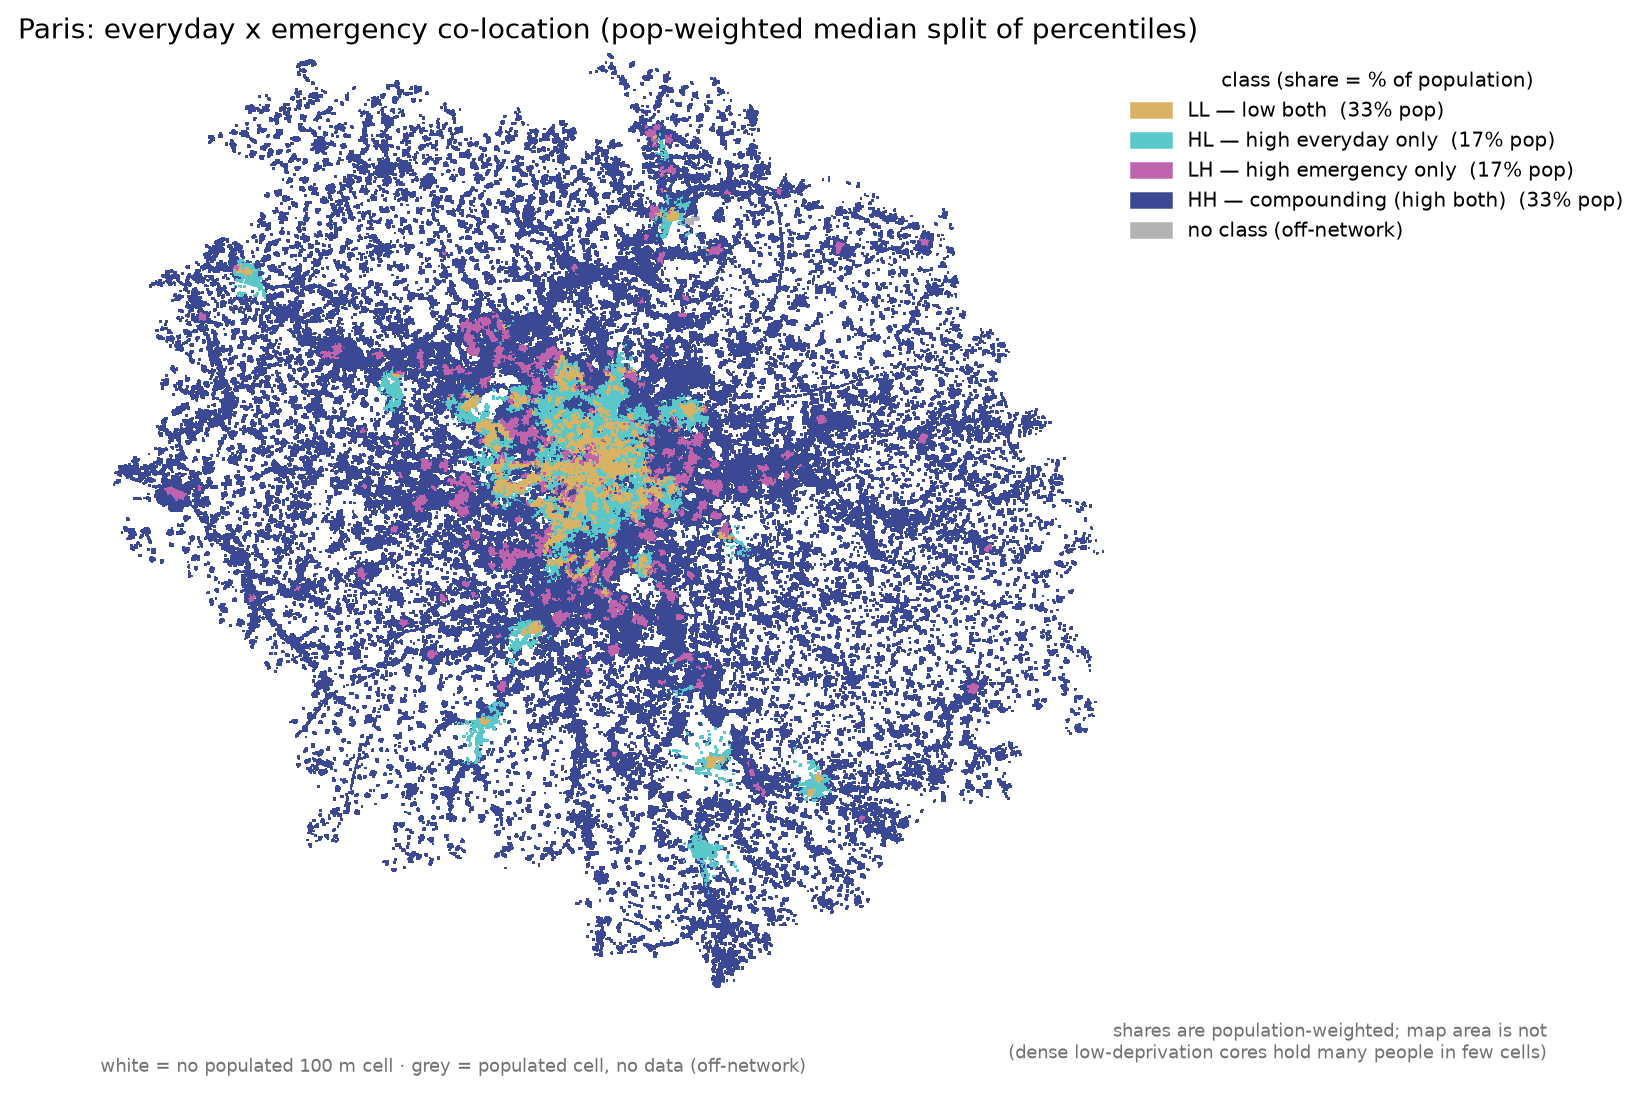
\includegraphics[width=0.48\textwidth]{paris.png}%
\hfill
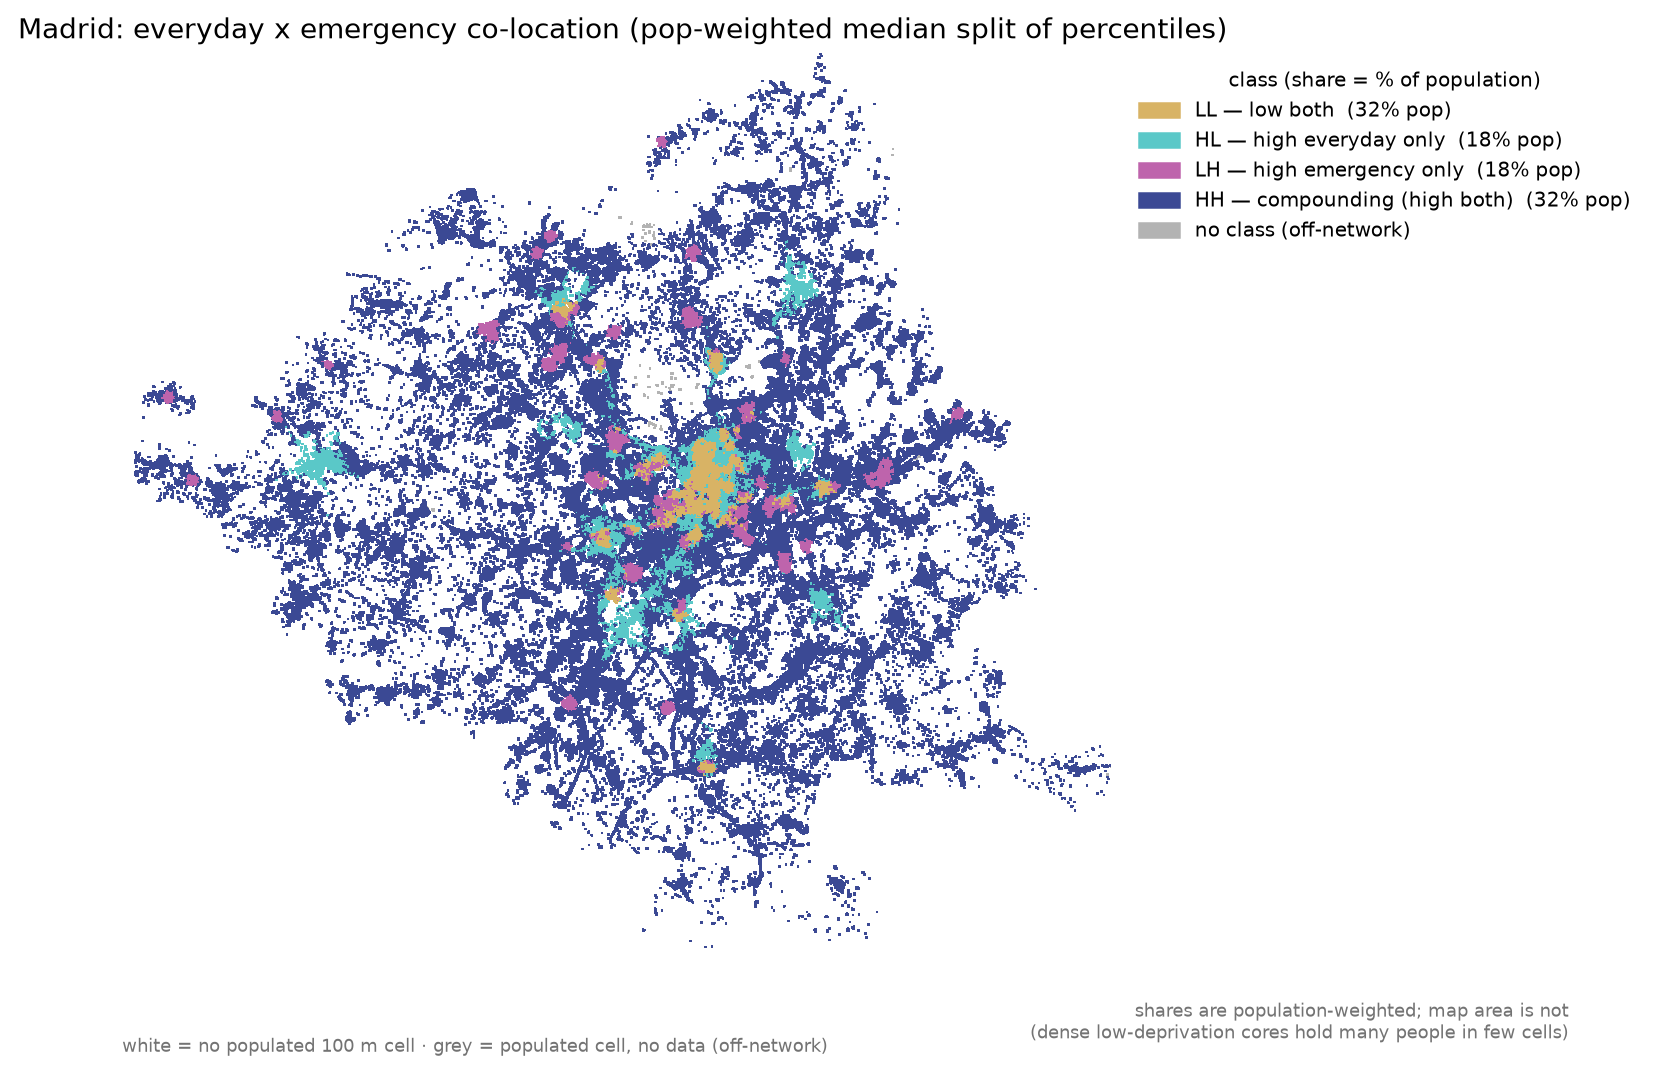
\includegraphics[width=0.48\textwidth]{madrid.png}%
\\[2pt]
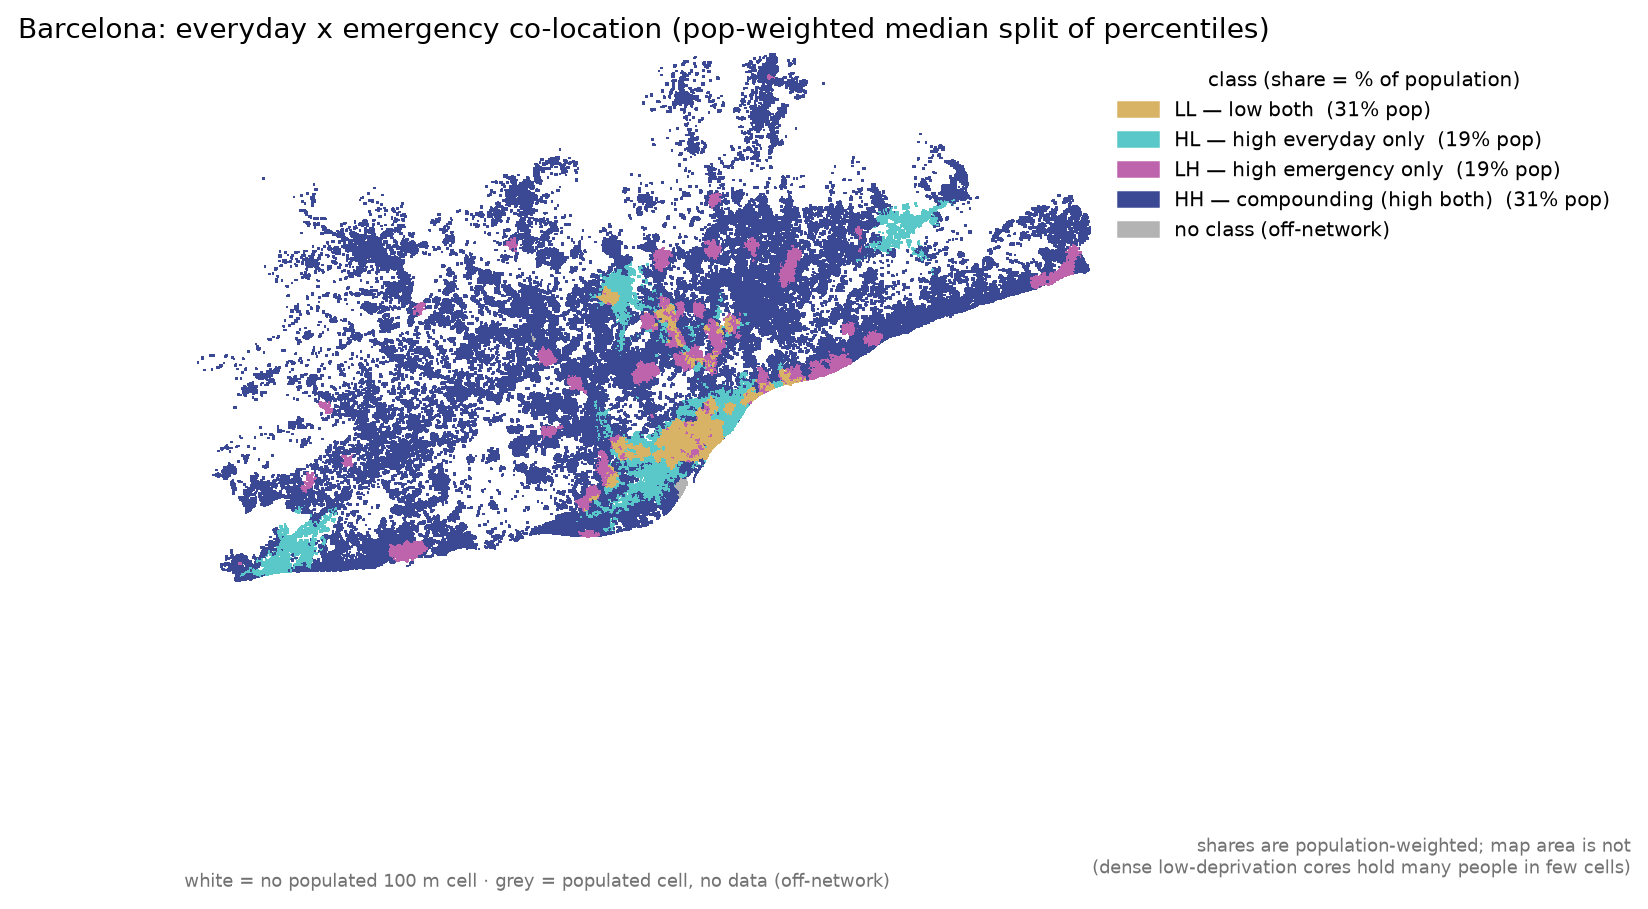
\includegraphics[width=0.48\textwidth]{barcelona.png}%
\hfill

\includegraphics[width=0.48\textwidth]{milano.png}%
\\[2pt]
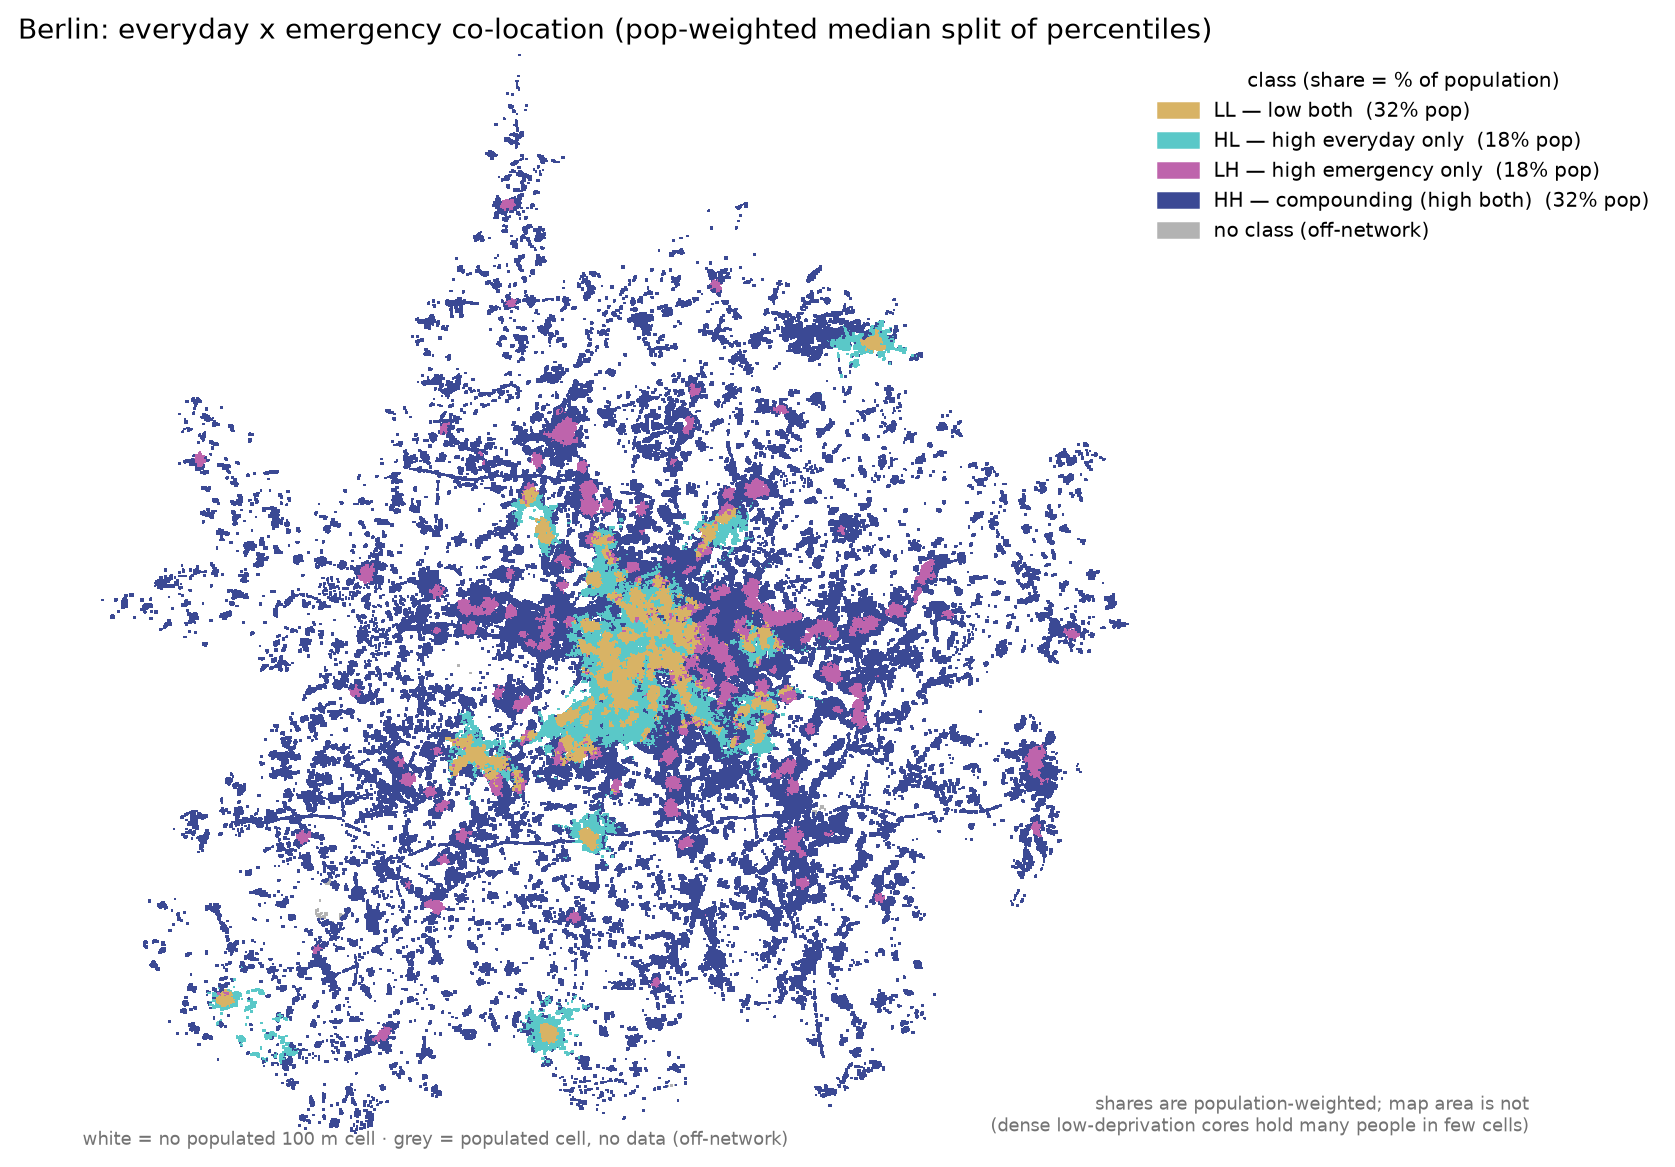
\includegraphics[width=0.48\textwidth]{berlin.png}%
\hfill

\includegraphics[width=0.48\textwidth]{roma.png}%
\\[2pt]
\caption{Per-city compounding maps (median-split co-location typology), cities 1--6 by population: Paris (FR), Madrid (ES), Barcelona (ES), Milano (IT), Berlin (DE), Roma (IT). Read for spatial pattern only; per-cell classes carry a $\sim$24\,\% routing-engine flip share (E.1).}
\label{fig:si-gallery-1}
\end{figure}

\begin{figure}[p]
\centering
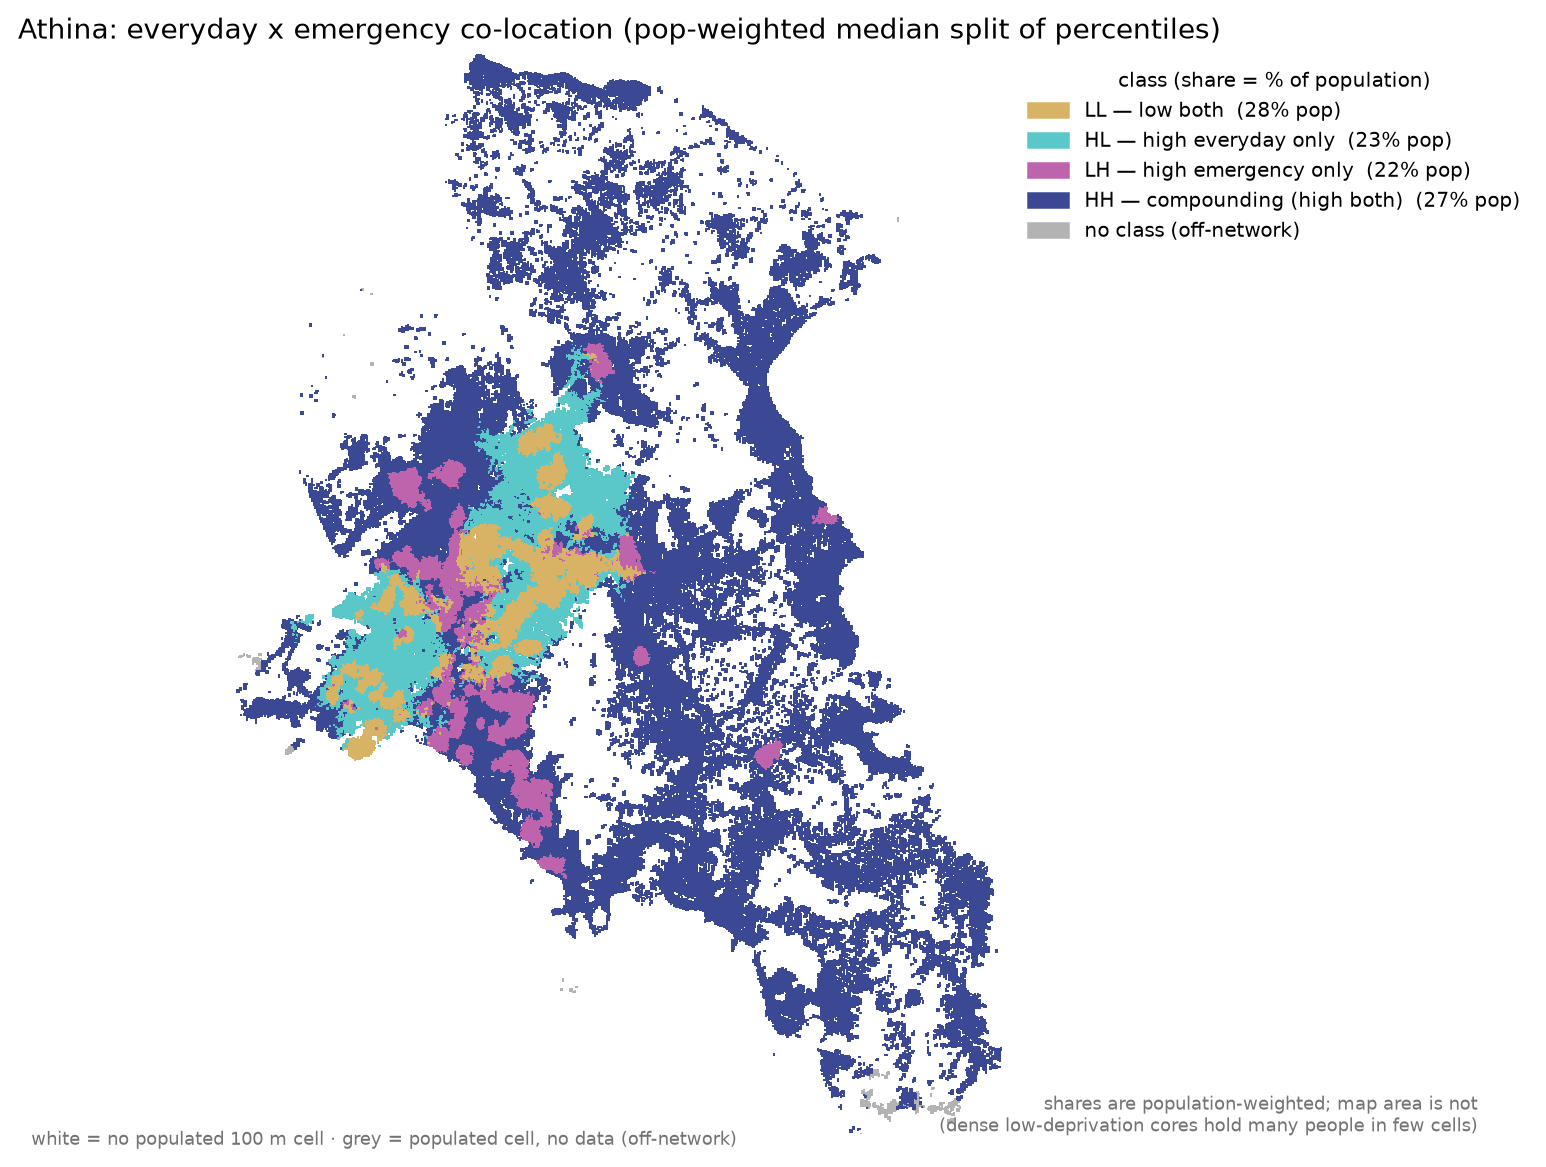
\includegraphics[width=0.48\textwidth]{athina.png}%
\hfill

\includegraphics[width=0.48\textwidth]{bruxelles.png}%
\\[2pt]
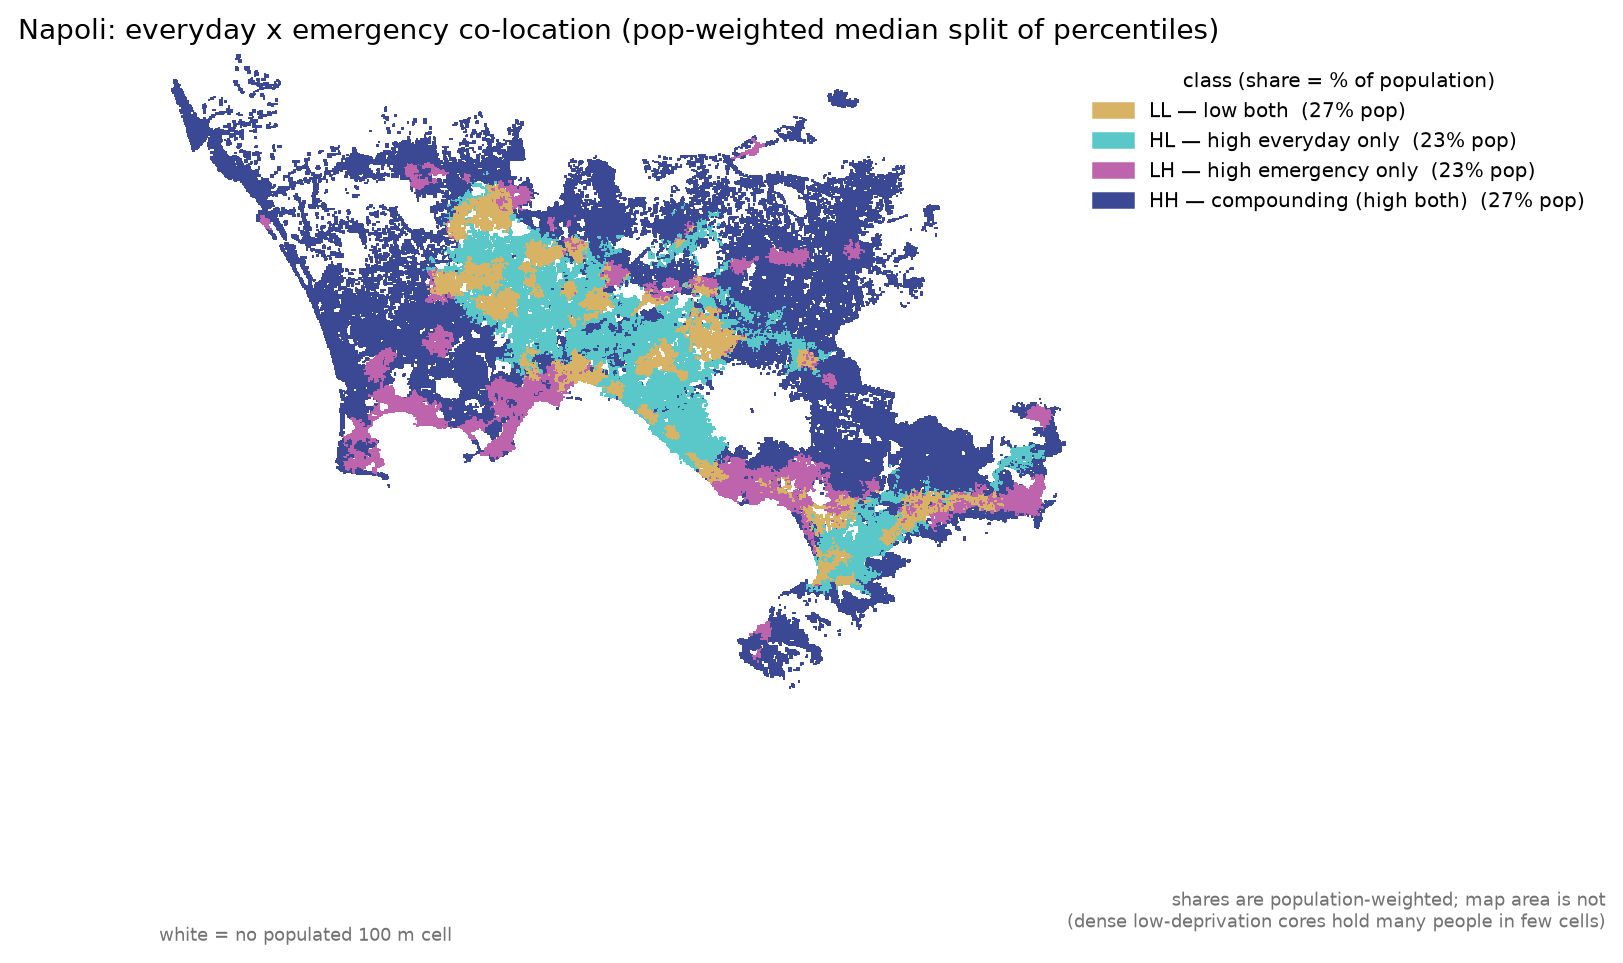
\includegraphics[width=0.48\textwidth]{napoli.png}%
\hfill

\includegraphics[width=0.48\textwidth]{warszawa.png}%
\\[2pt]
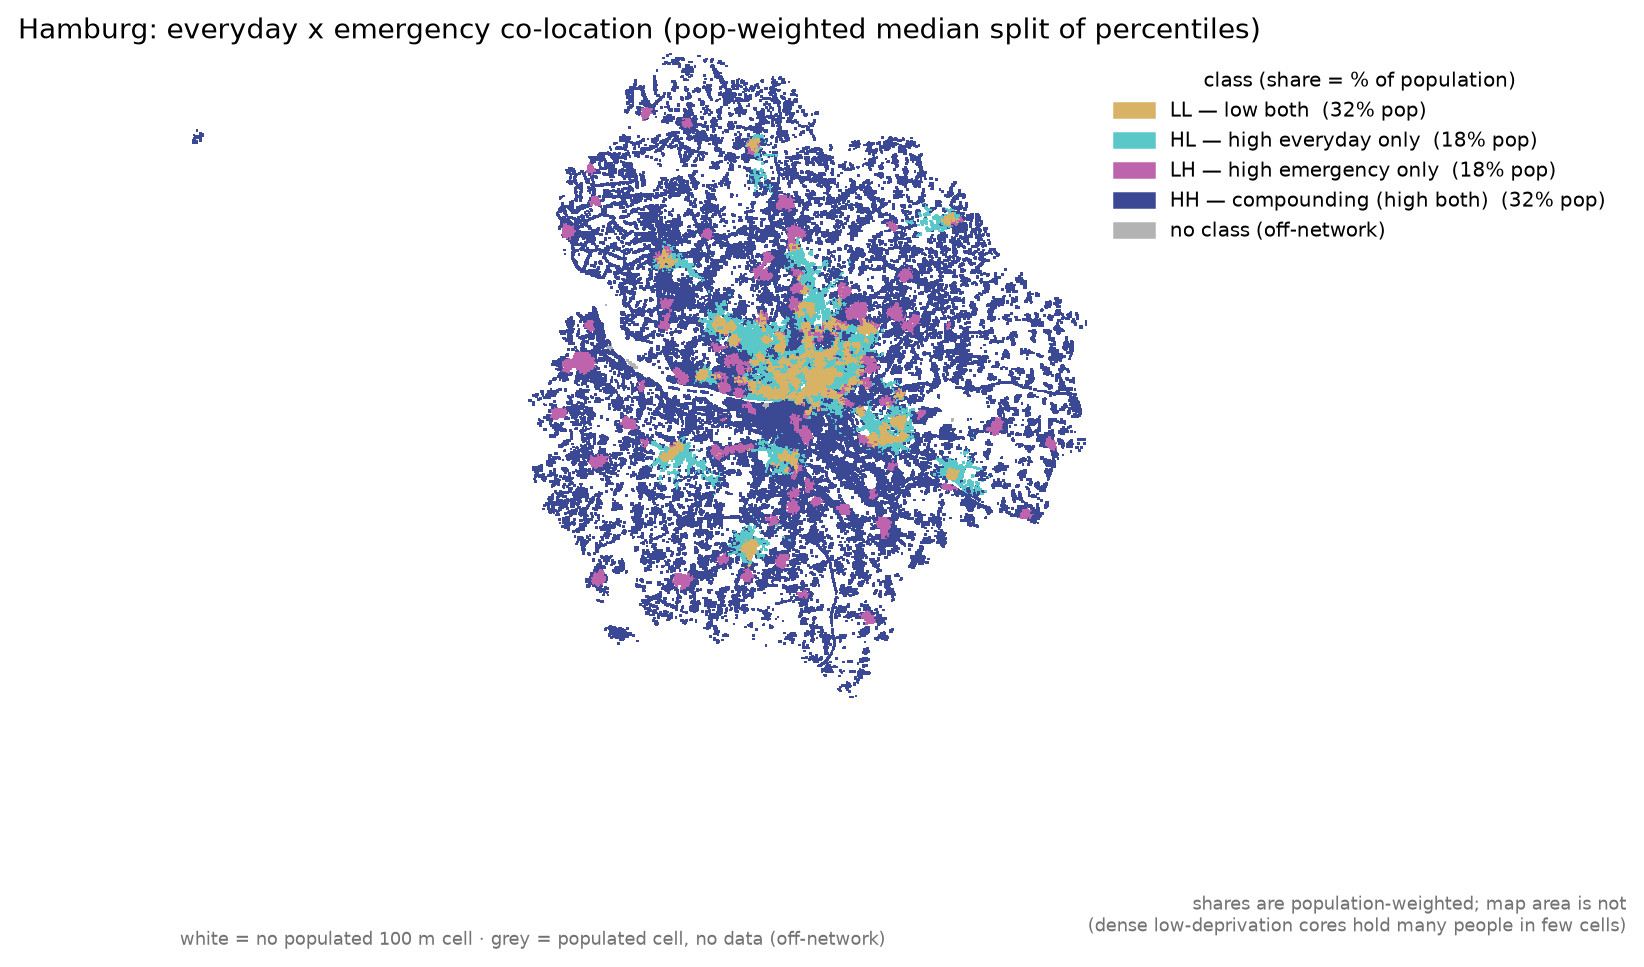
\includegraphics[width=0.48\textwidth]{hamburg.png}%
\hfill

\includegraphics[width=0.48\textwidth]{bucuresti.png}%
\\[2pt]
\caption{Per-city compounding maps (median-split co-location typology), cities 7--12 by population: Athina (EL), Bruxelles (BE), Napoli (IT), Warszawa (PL), Hamburg (DE), Bucure{\c{s}}ti (RO). Read for spatial pattern only; per-cell classes carry a $\sim$24\,\% routing-engine flip share (E.1).}
\label{fig:si-gallery-2}
\end{figure}

\begin{figure}[p]
\centering
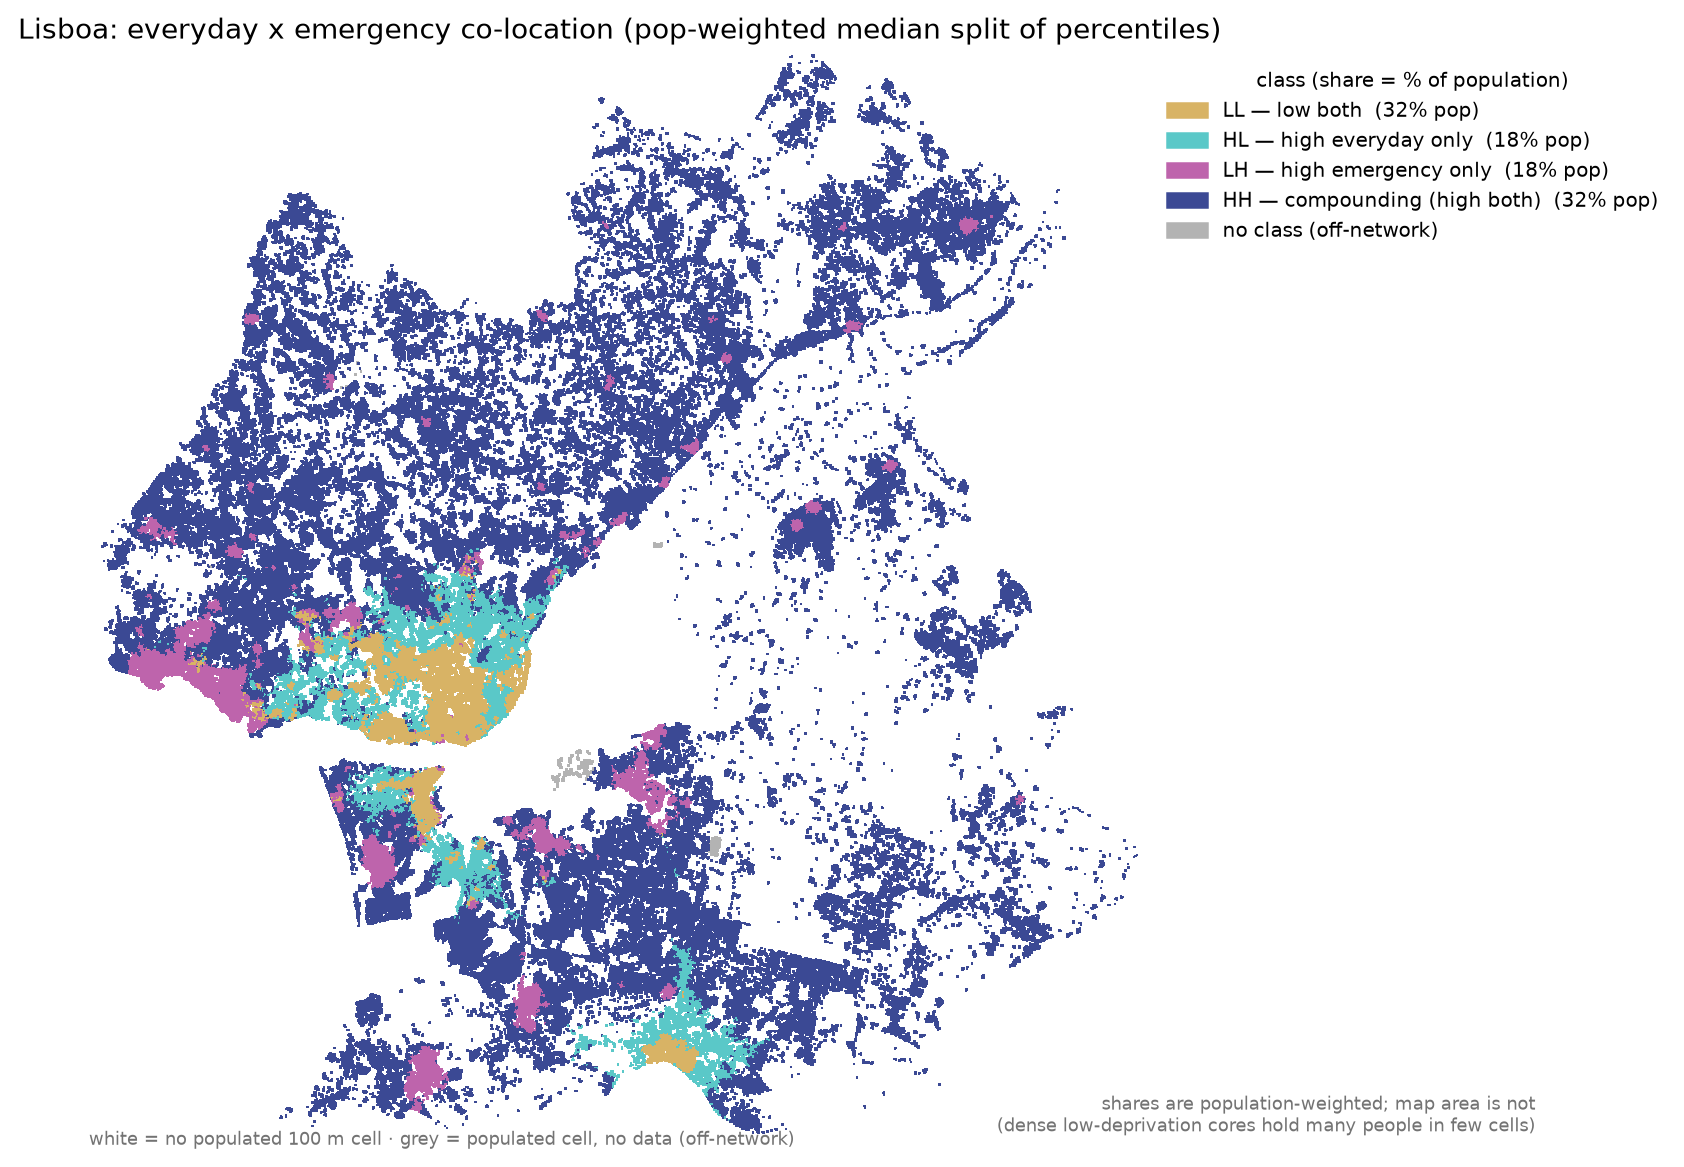
\includegraphics[width=0.48\textwidth]{lisboa.png}%
\hfill

\includegraphics[width=0.48\textwidth]{munchen.png}%
\\[2pt]

\includegraphics[width=0.48\textwidth]{budapest.png}%
\hfill

\includegraphics[width=0.48\textwidth]{amsterdam.png}%
\\[2pt]

\includegraphics[width=0.48\textwidth]{stockholm.png}%
\hfill
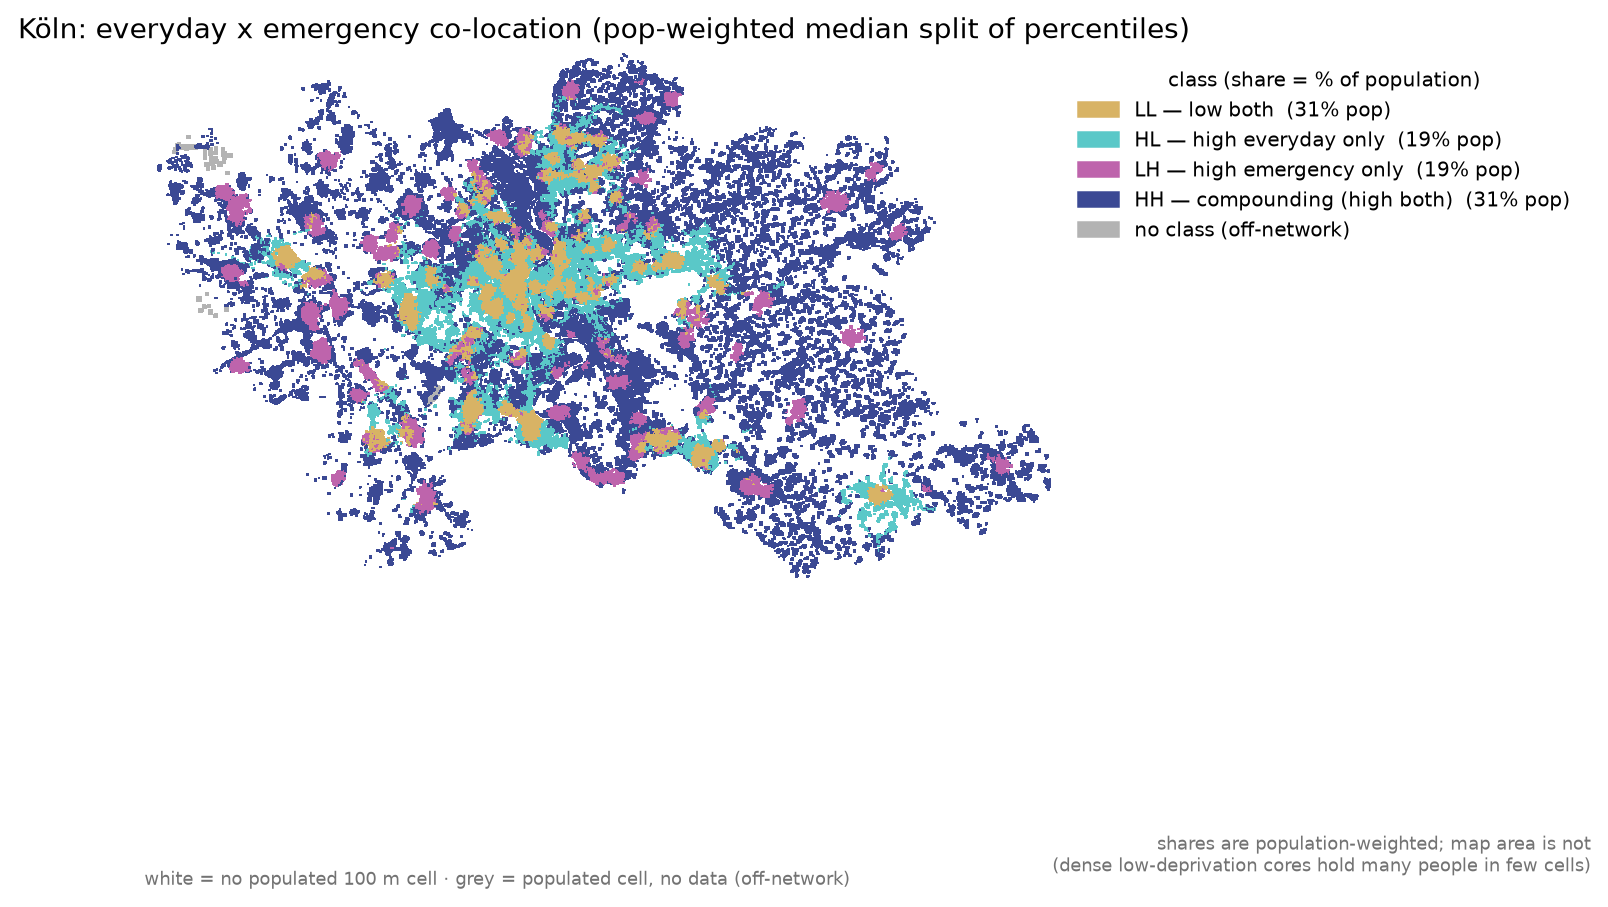
\includegraphics[width=0.48\textwidth]{koeln.png}%
\\[2pt]
\caption{Per-city compounding maps (median-split co-location typology), cities 13--18 by population: Lisboa (PT), M{\"u}nchen (DE), Budapest (HU), Amsterdam (NL), Stockholm (SE), K{\"o}ln (DE). Read for spatial pattern only; per-cell classes carry a $\sim$24\,\% routing-engine flip share (E.1).}
\label{fig:si-gallery-3}
\end{figure}

\begin{figure}[p]
\centering
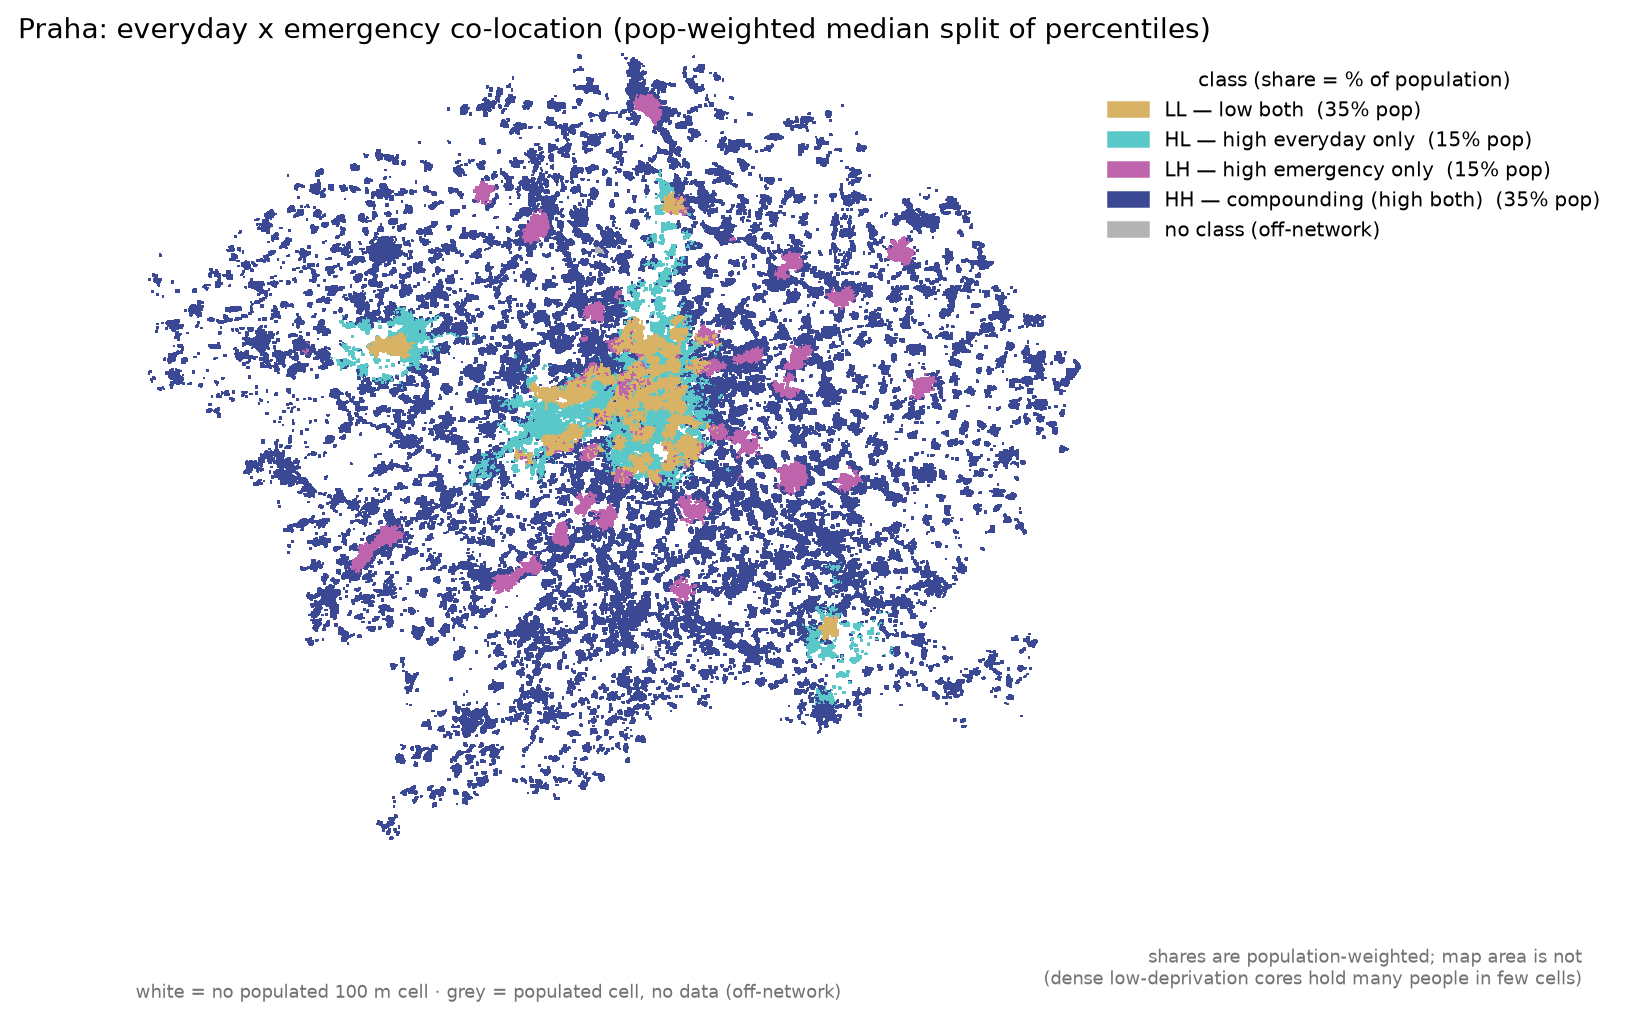
\includegraphics[width=0.48\textwidth]{praha.png}%
\hfill

\includegraphics[width=0.48\textwidth]{kobenhavn.png}%
\\[2pt]
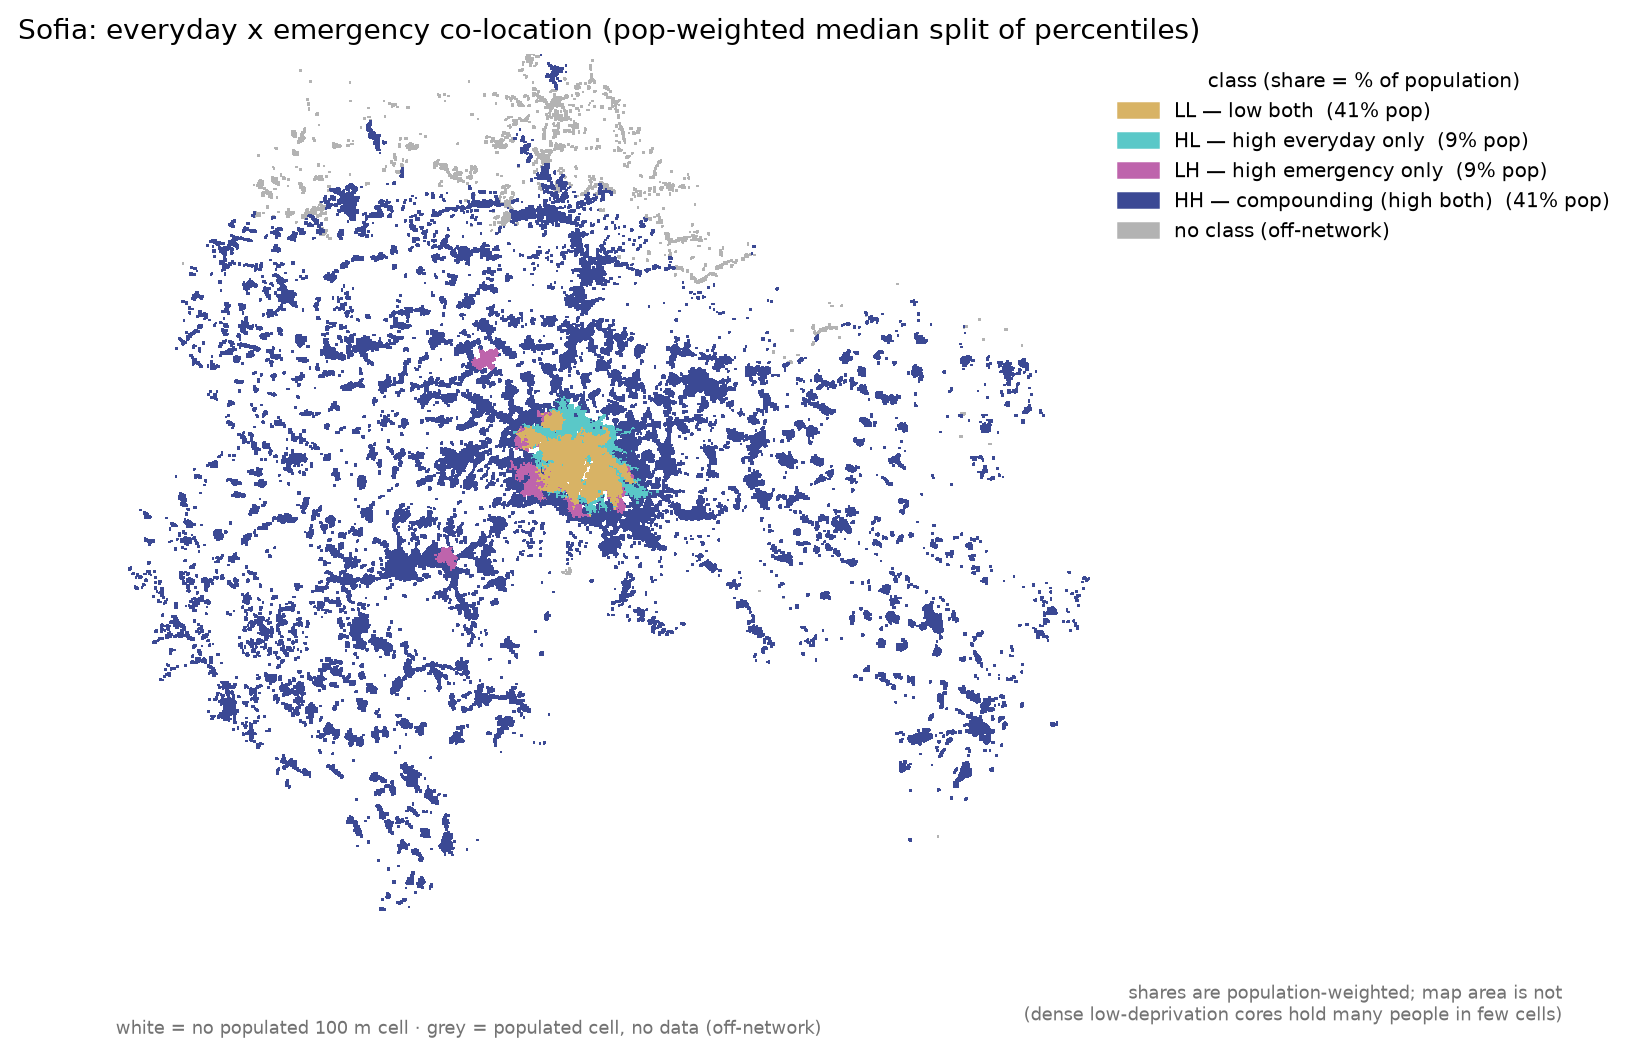
\includegraphics[width=0.48\textwidth]{sofia.png}%
\hfill

\includegraphics[width=0.48\textwidth]{helsinki.png}%
\\[2pt]

\includegraphics[width=0.48\textwidth]{oslo.png}%
\hfill
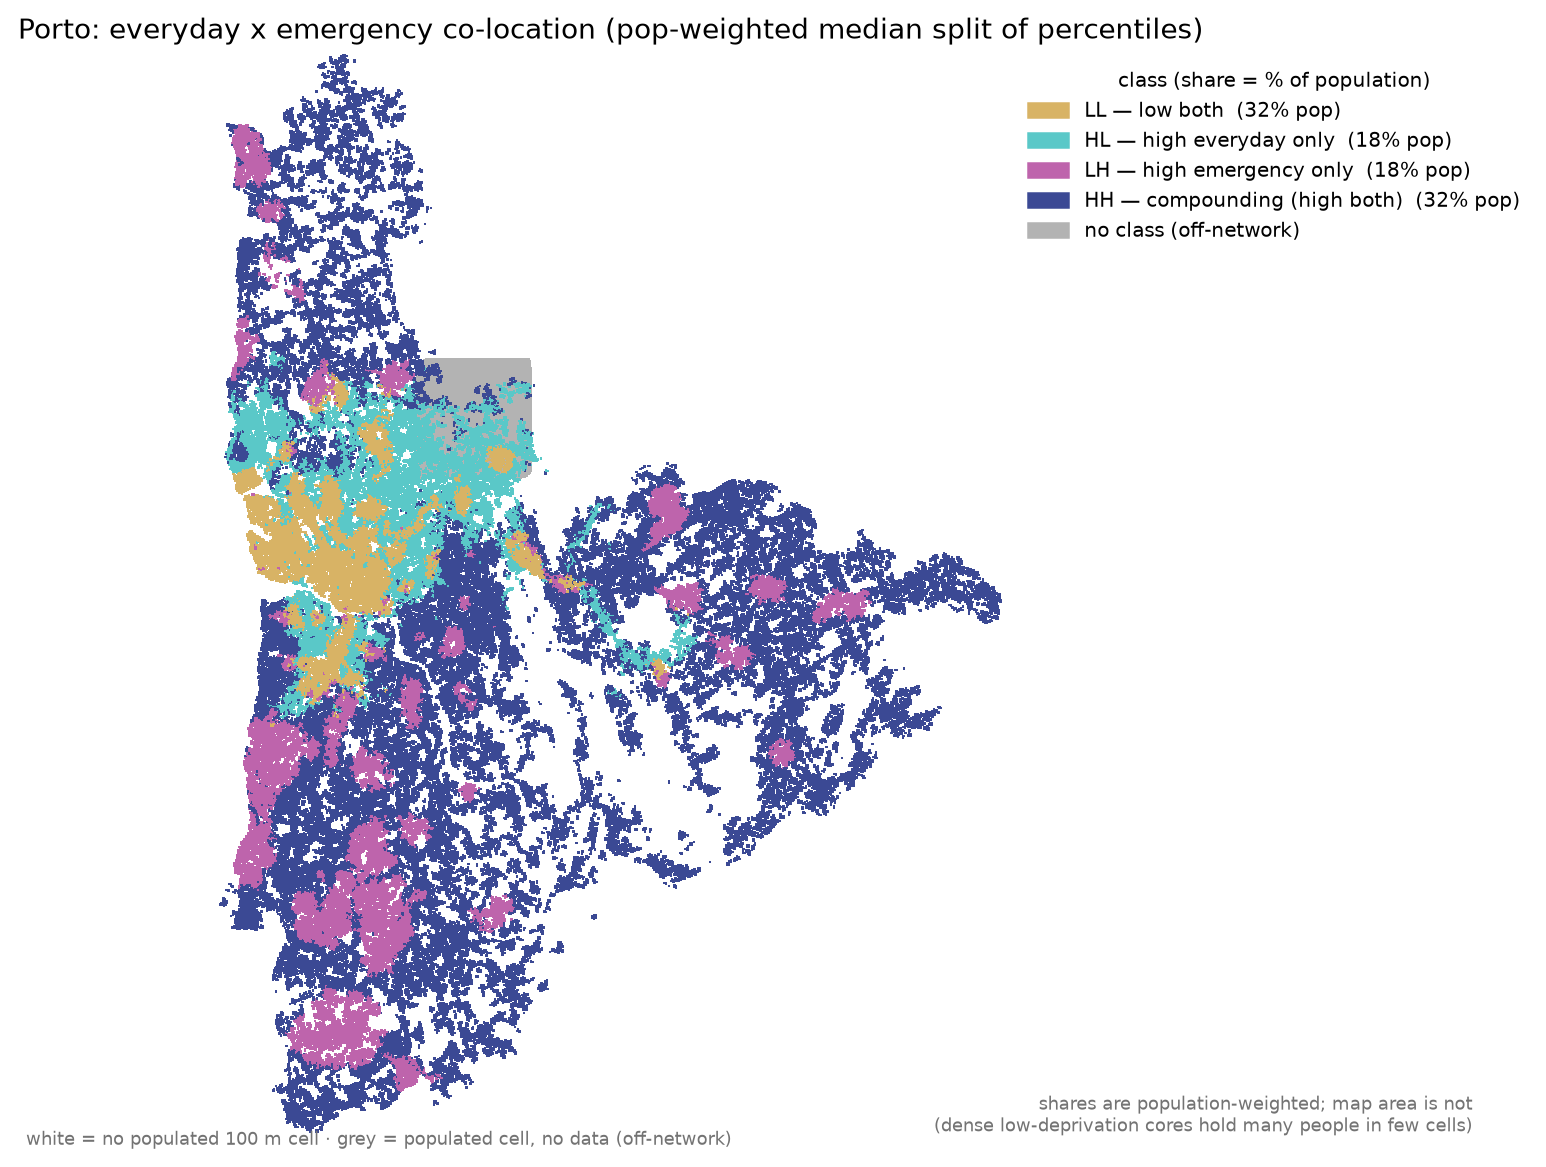
\includegraphics[width=0.48\textwidth]{porto.png}%
\\[2pt]
\caption{Per-city compounding maps (median-split co-location typology), cities 19--24 by population: Praha (CZ), K{\o{}}benhavn (DK), Sofia (BG), Helsinki (FI), Oslo (NO), Porto (PT). Read for spatial pattern only; per-cell classes carry a $\sim$24\,\% routing-engine flip share (E.1).}
\label{fig:si-gallery-4}
\end{figure}

\begin{figure}[p]
\centering
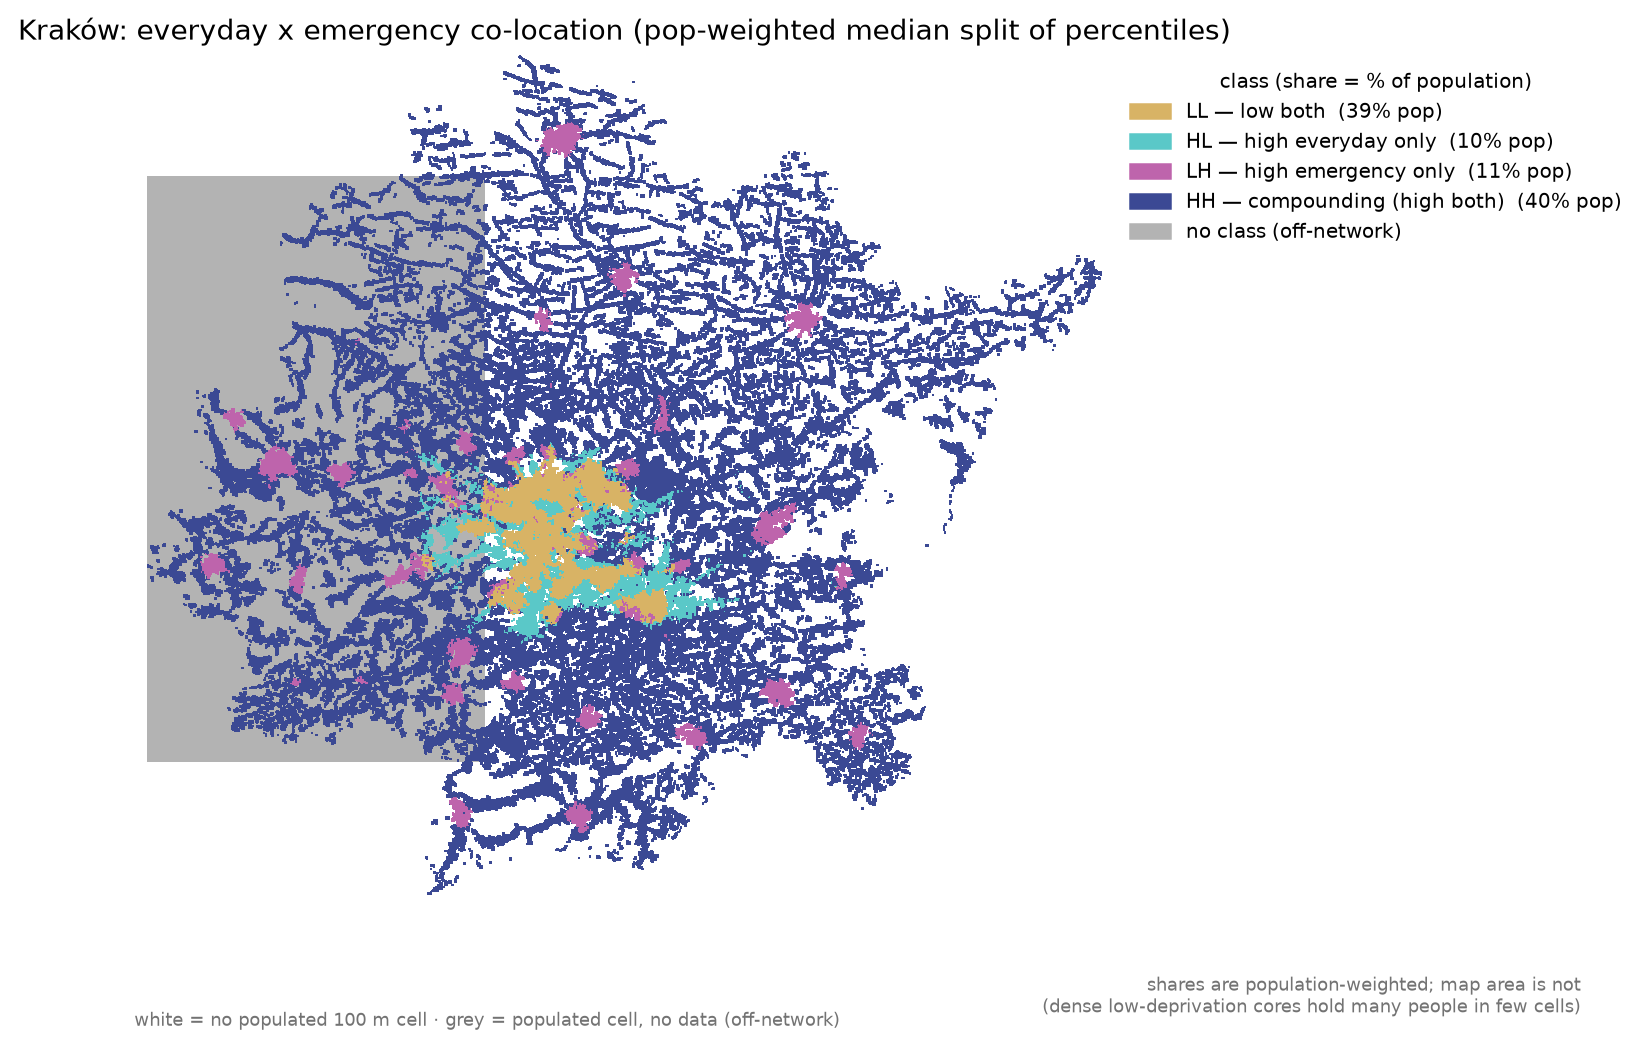
\includegraphics[width=0.48\textwidth]{krakow.png}%
\hfill

\includegraphics[width=0.48\textwidth]{katowice.png}%
\\[2pt]
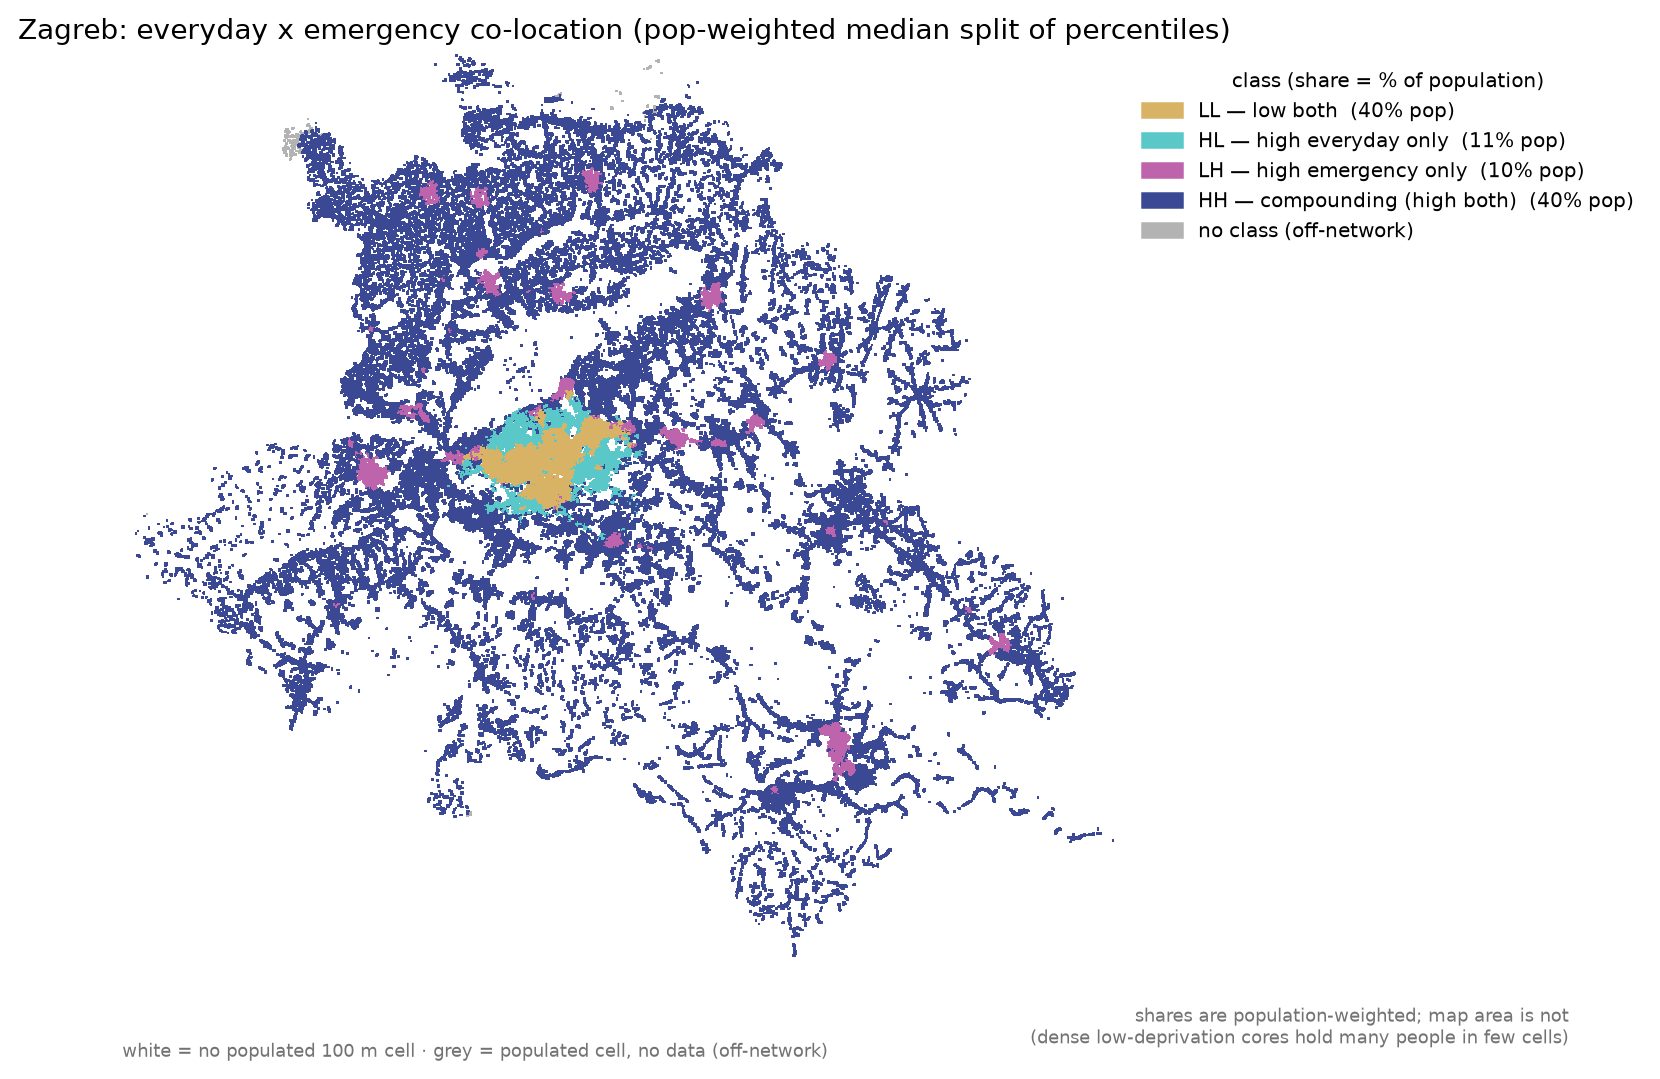
\includegraphics[width=0.48\textwidth]{zagreb.png}%
\hfill

\includegraphics[width=0.48\textwidth]{antwerpen.png}%
\\[2pt]
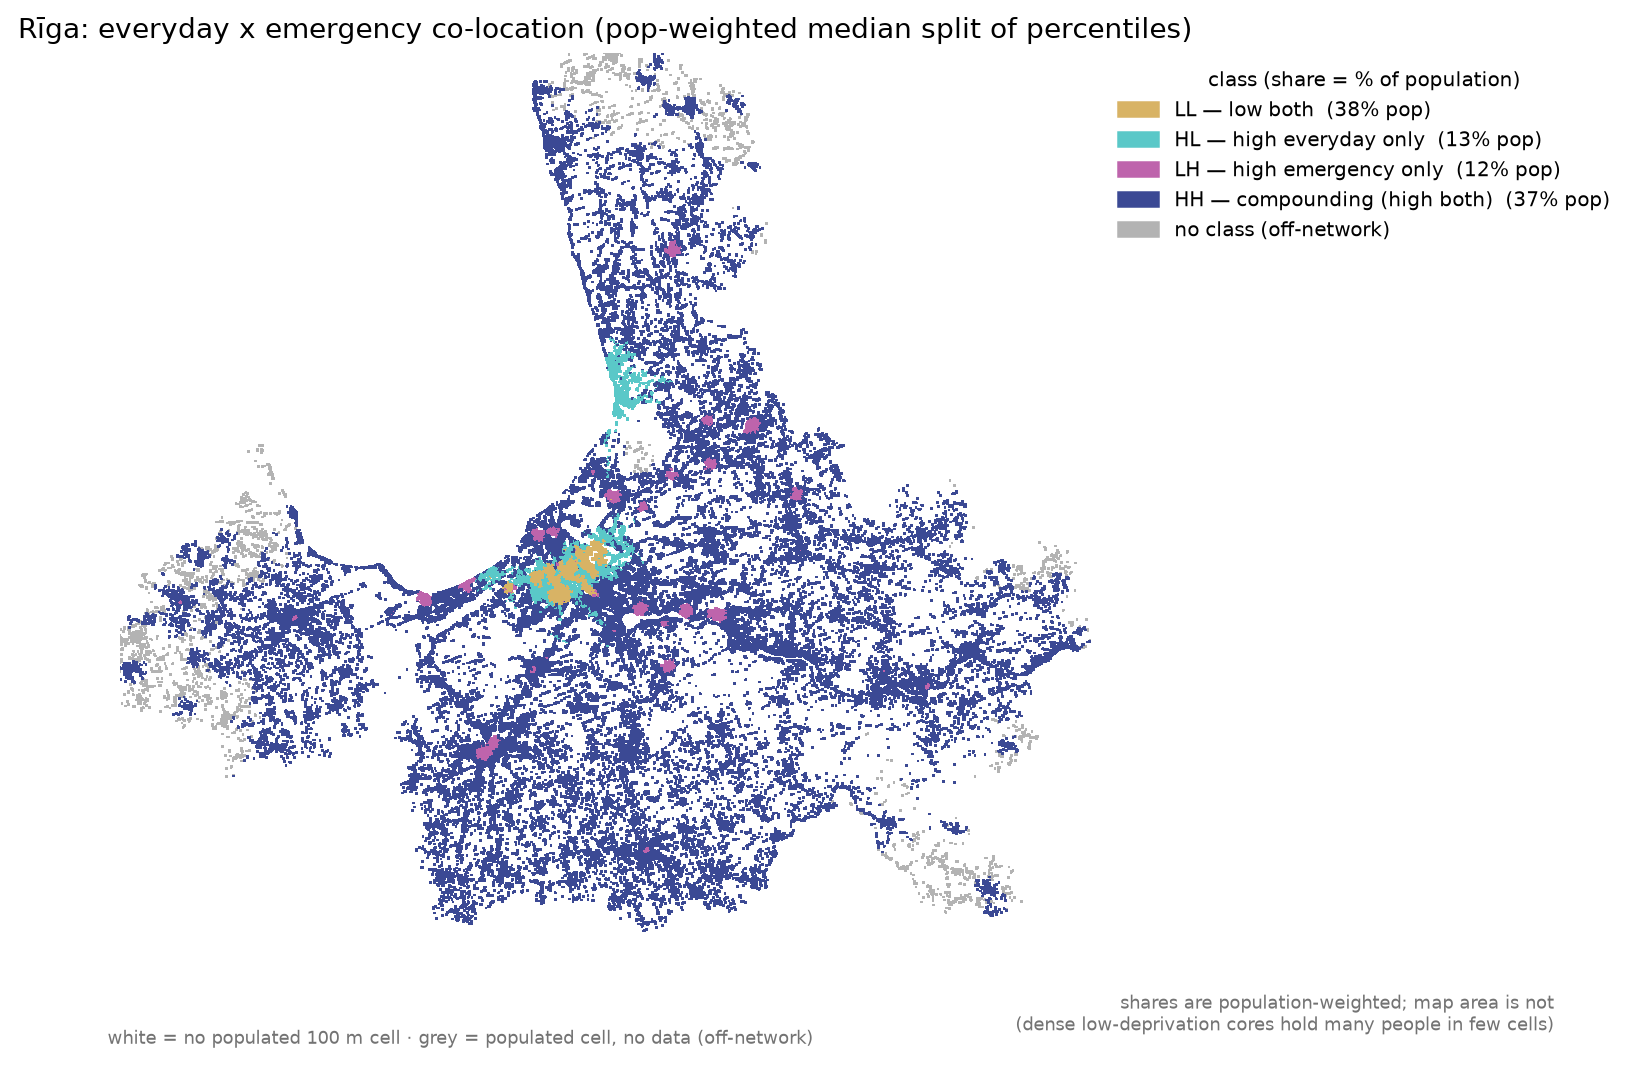
\includegraphics[width=0.48\textwidth]{riga.png}%
\hfill

\includegraphics[width=0.48\textwidth]{bilbao.png}%
\\[2pt]
\caption{Per-city compounding maps (median-split co-location typology), cities 25--30 by population: Krak{\'o}w (PL), Katowice (PL), Zagreb (HR), Antwerpen (BE), R{\={\i}}ga (LV), Bilbao (ES). Read for spatial pattern only; per-cell classes carry a $\sim$24\,\% routing-engine flip share (E.1).}
\label{fig:si-gallery-5}
\end{figure}

\begin{figure}[p]
\centering

\includegraphics[width=0.48\textwidth]{lodz.png}%
\hfill
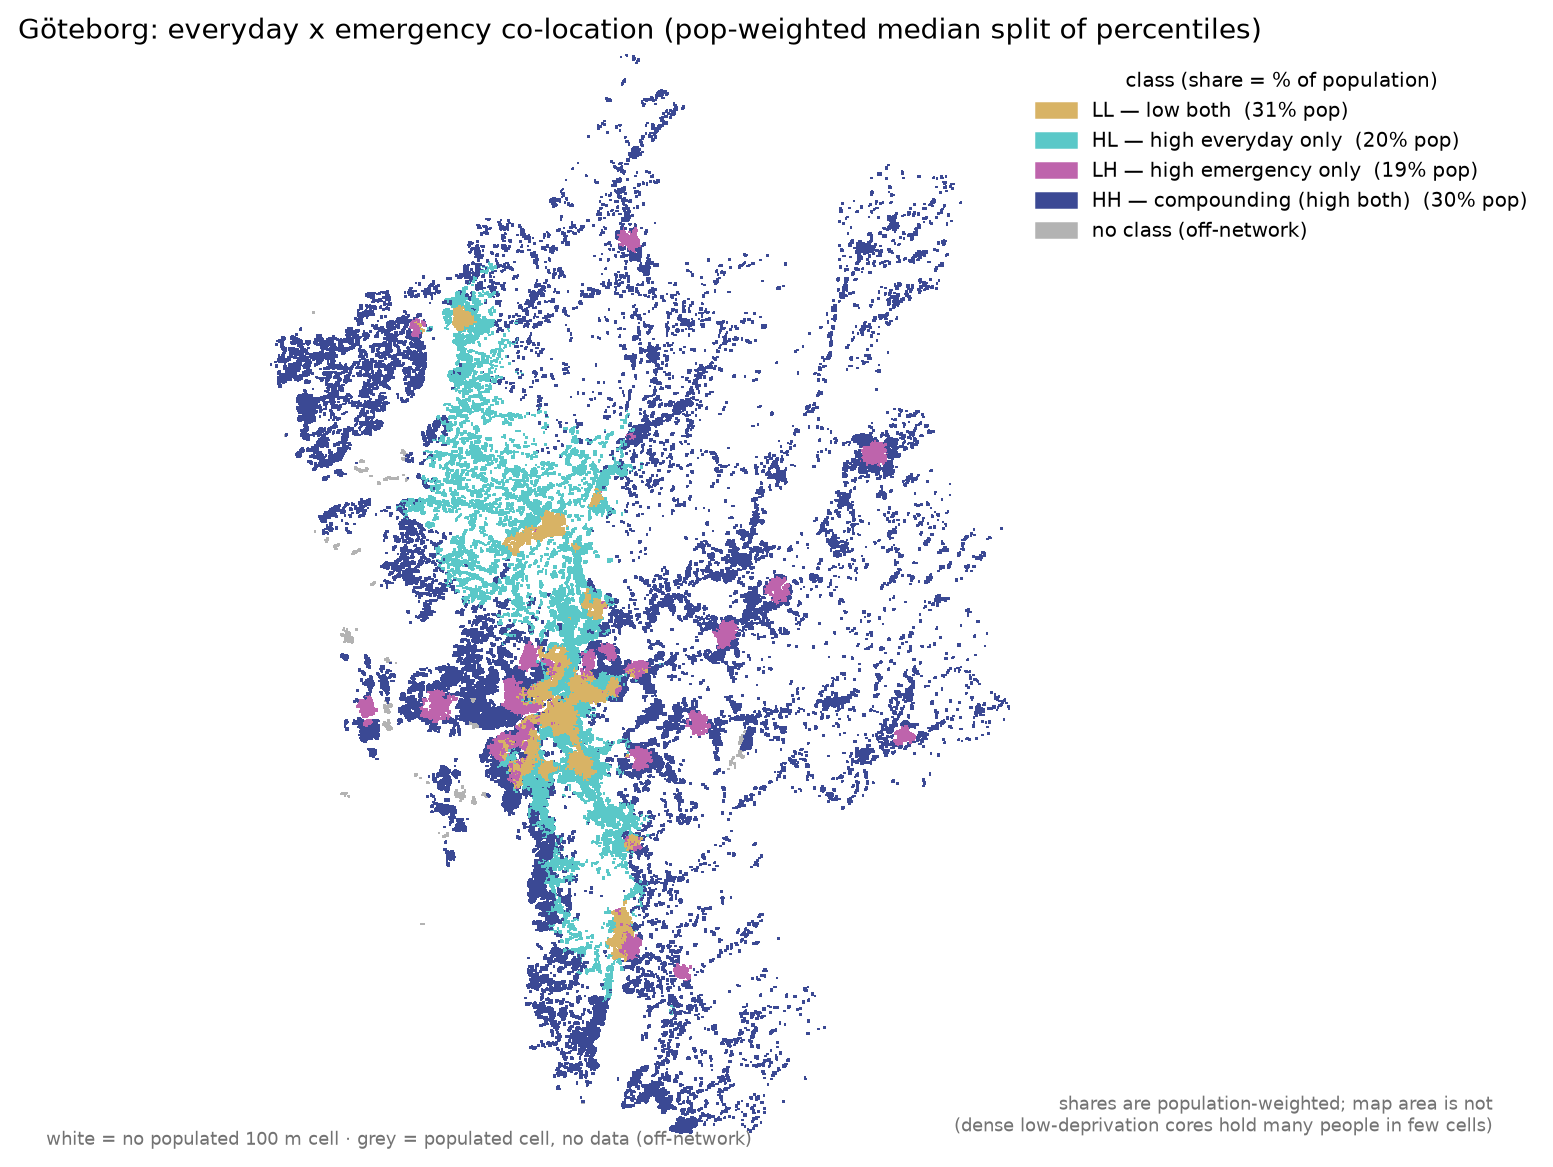
\includegraphics[width=0.48\textwidth]{goteborg.png}%
\\[2pt]
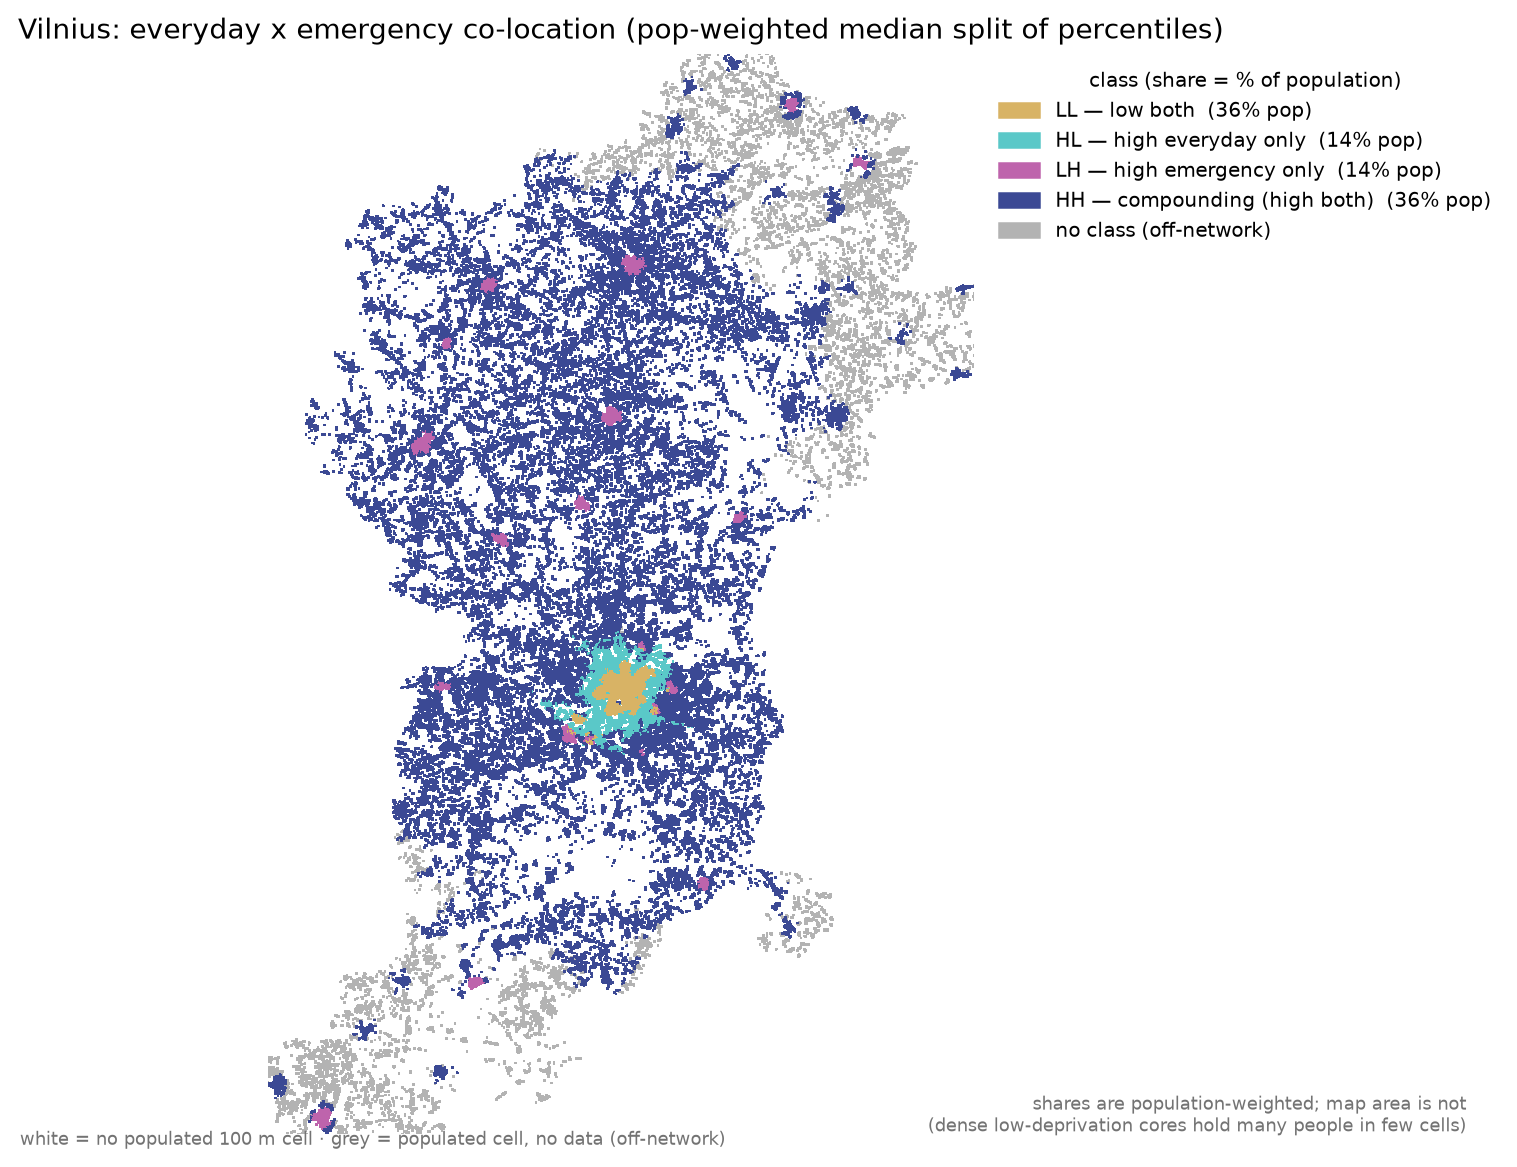
\includegraphics[width=0.48\textwidth]{vilnius.png}%
\hfill

\includegraphics[width=0.48\textwidth]{palermo.png}%
\\[2pt]

\includegraphics[width=0.48\textwidth]{alicante.png}%
\hfill
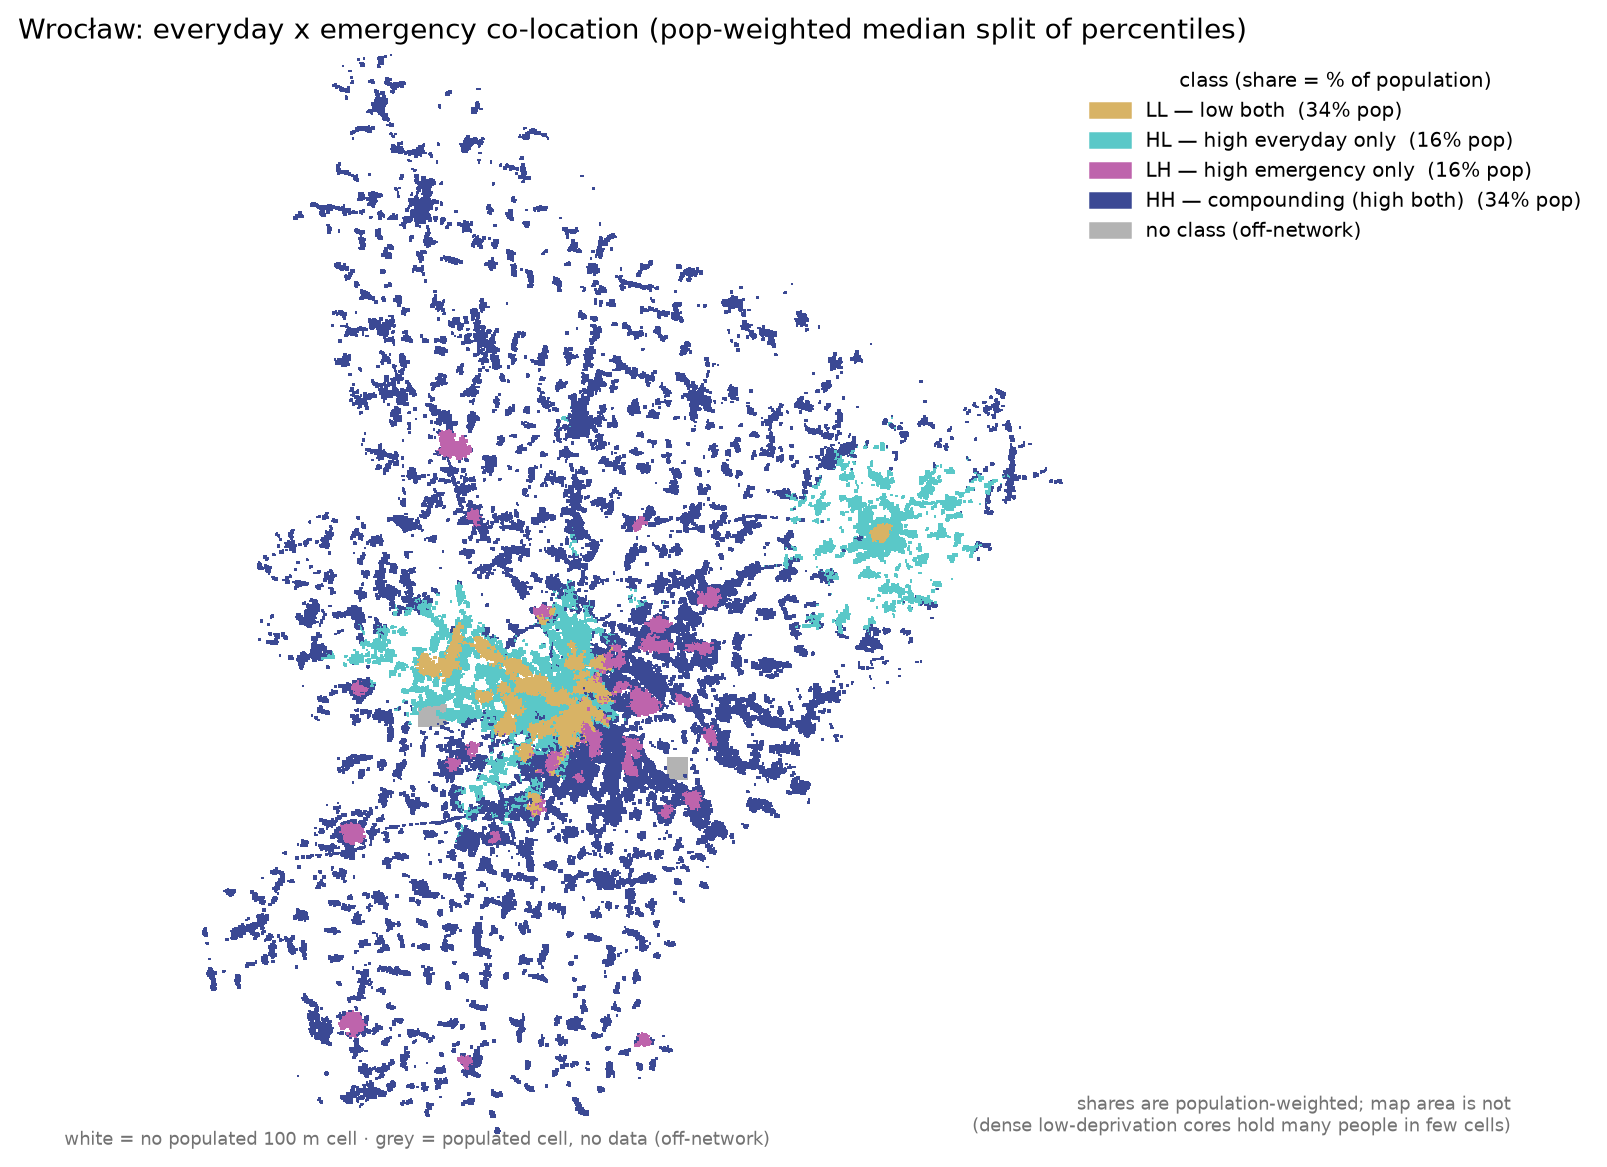
\includegraphics[width=0.48\textwidth]{wroclaw.png}%
\\[2pt]
\caption{Per-city compounding maps (median-split co-location typology), cities 31--36 by population: {\L{}}{\'o}d{\'z} (PL), G{\"o}teborg (SE), Vilnius (LT), Palermo (IT), Alicante (ES), Wroc{\l{}}aw (PL). Read for spatial pattern only; per-cell classes carry a $\sim$24\,\% routing-engine flip share (E.1).}
\label{fig:si-gallery-6}
\end{figure}

\begin{figure}[p]
\centering

\includegraphics[width=0.48\textwidth]{bratislava.png}%
\hfill

\includegraphics[width=0.48\textwidth]{ljubljana.png}%
\\[2pt]
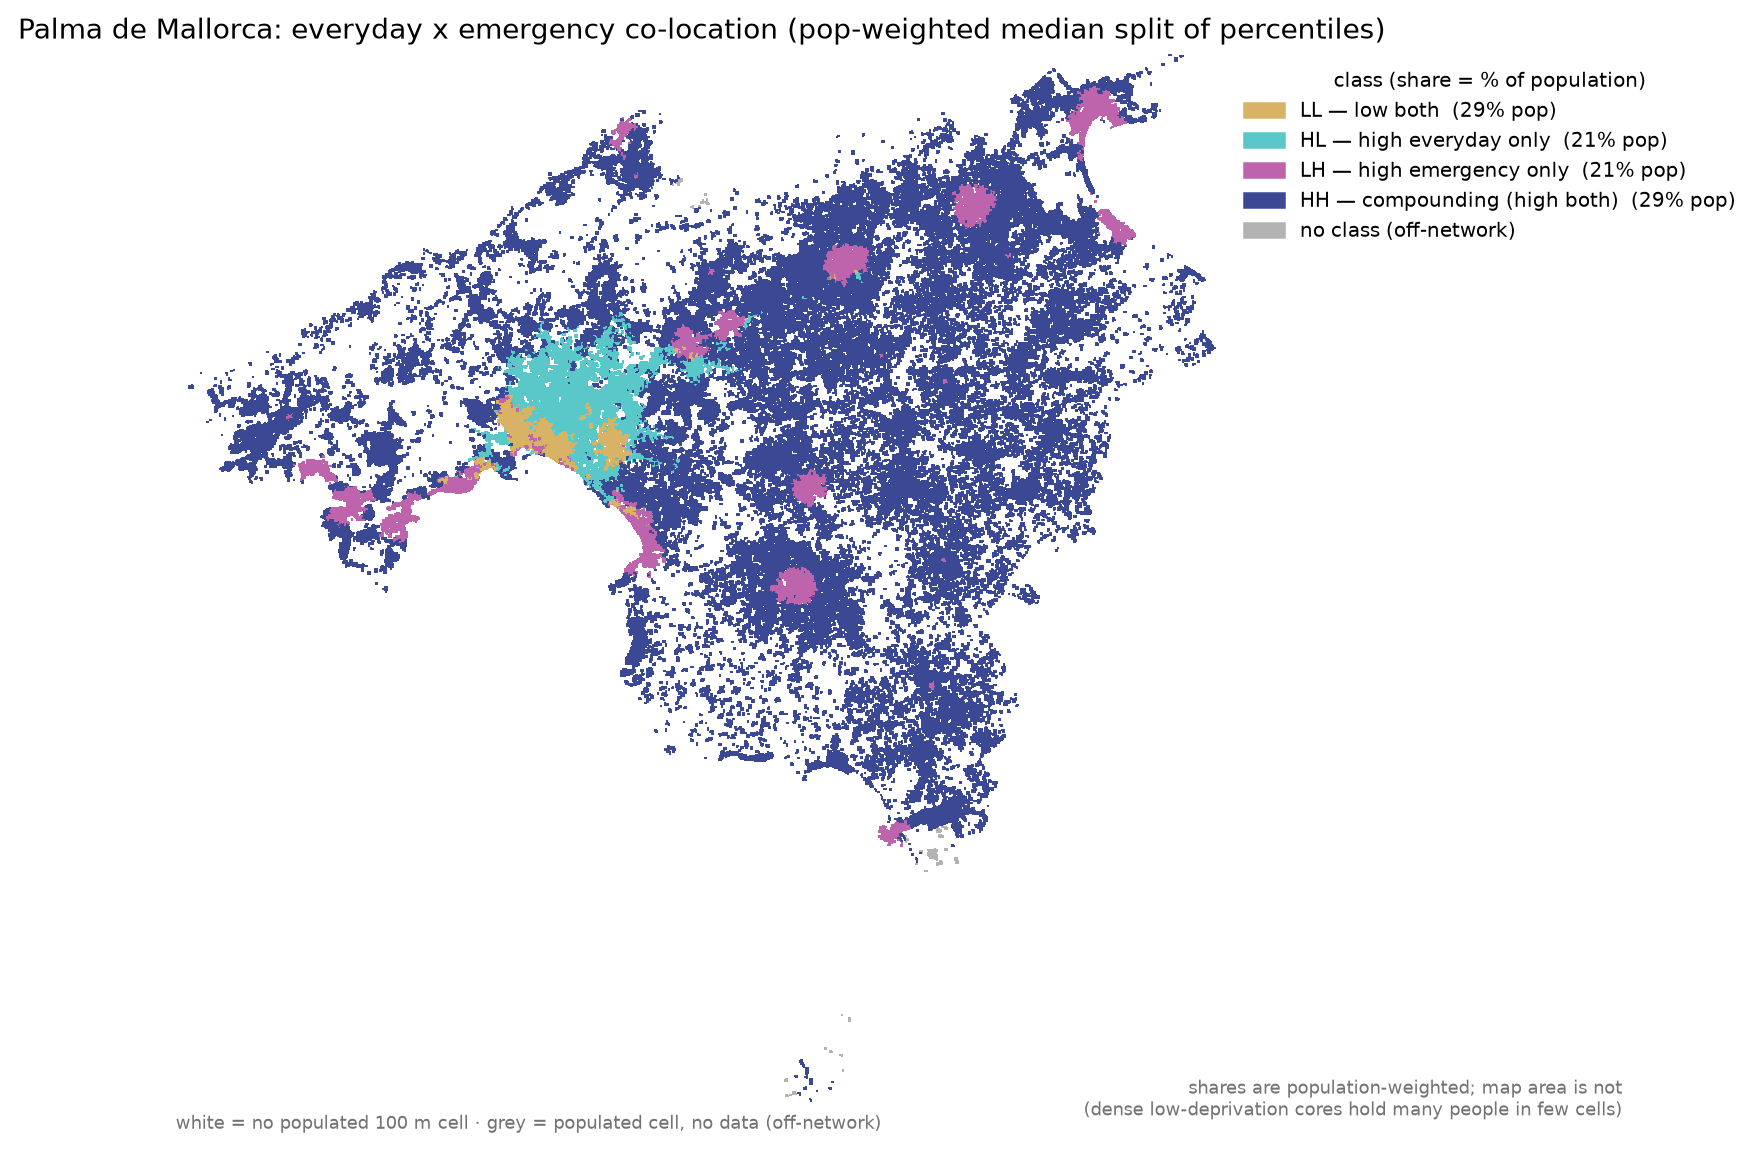
\includegraphics[width=0.48\textwidth]{palma_de_mallorca.png}%
\hfill
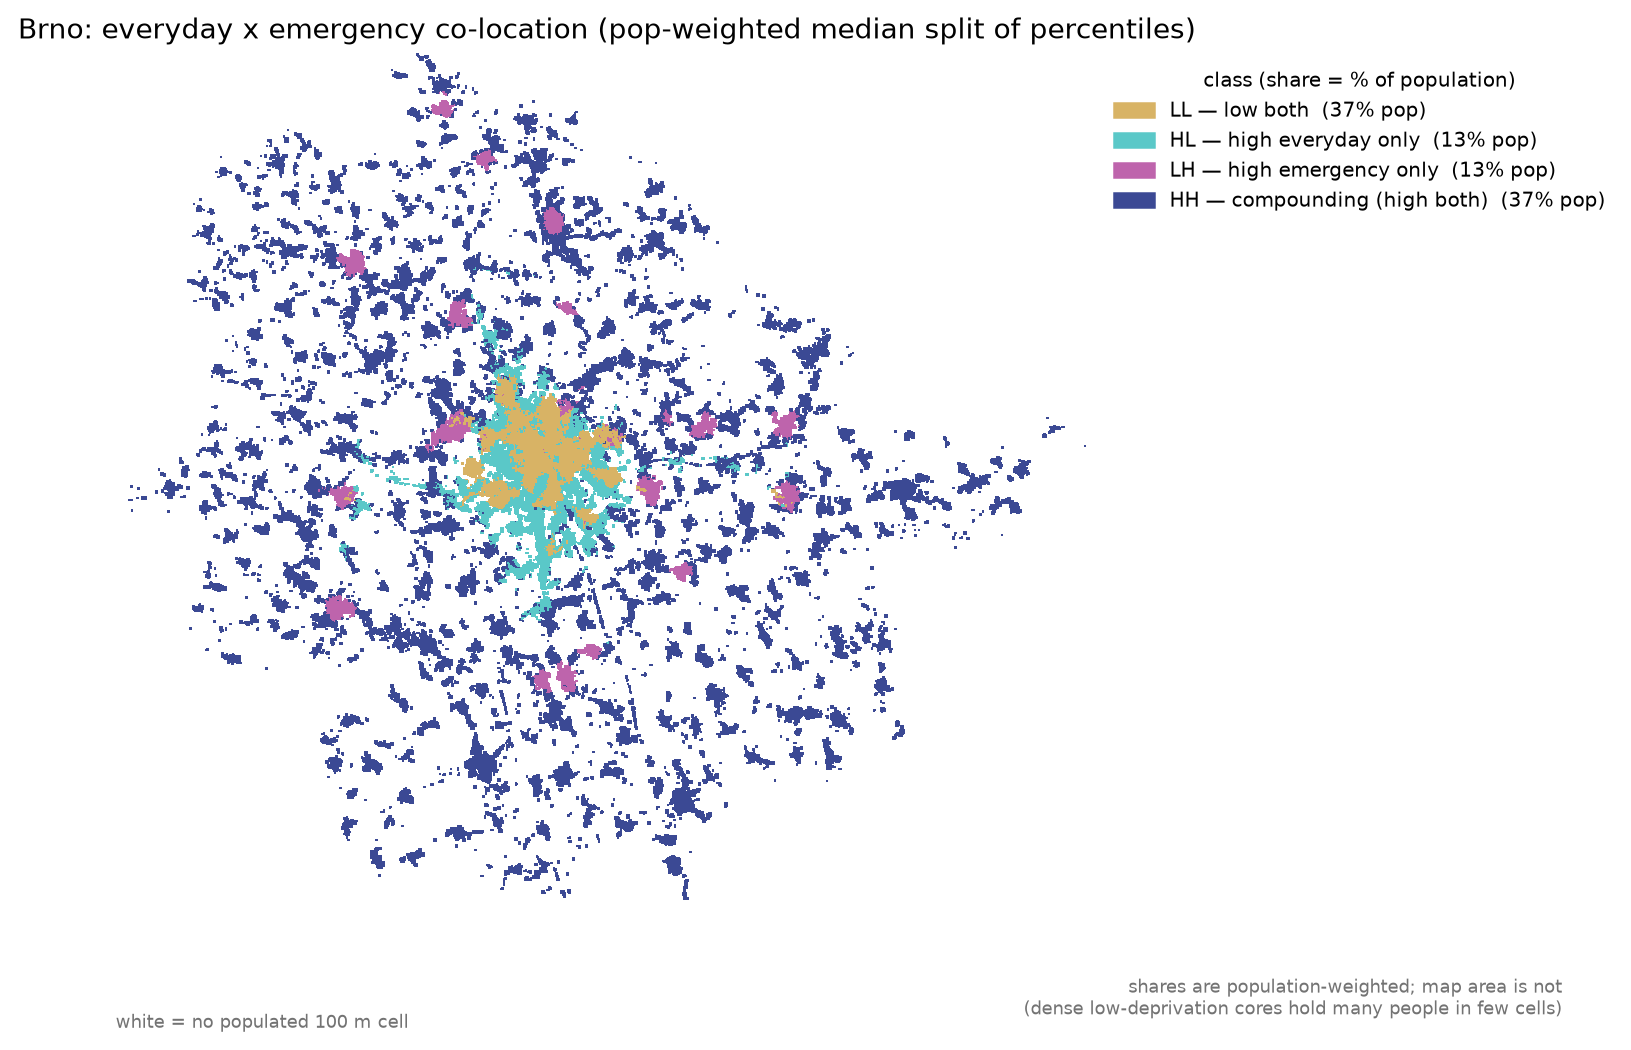
\includegraphics[width=0.48\textwidth]{brno.png}%
\\[2pt]
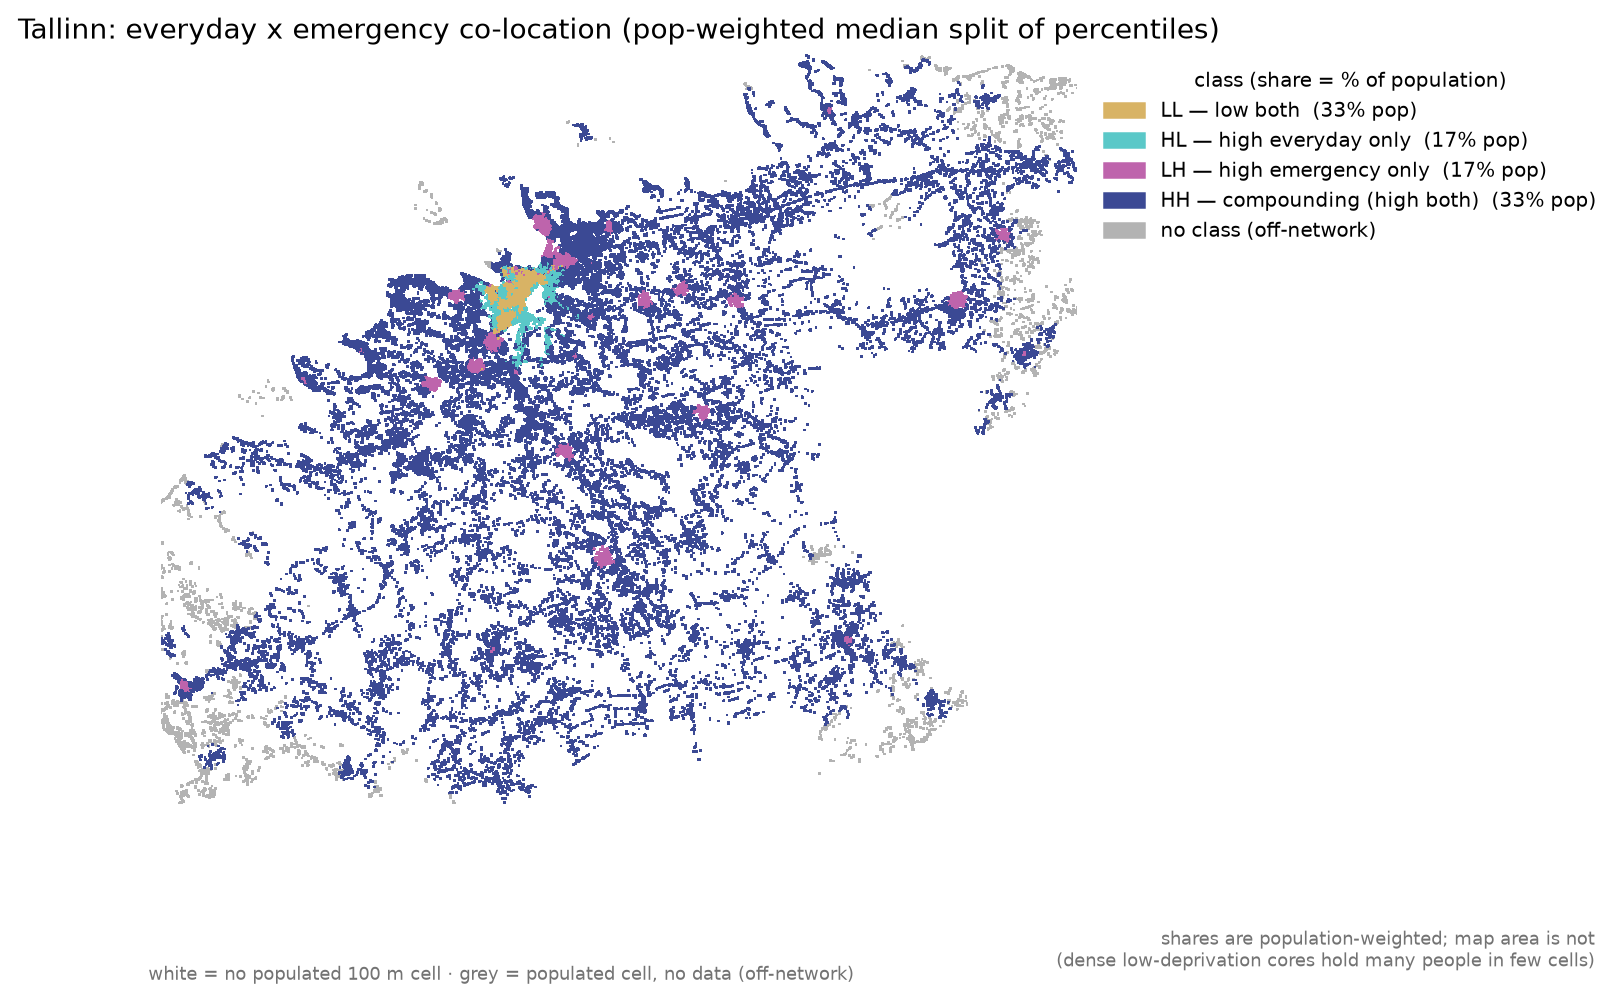
\includegraphics[width=0.48\textwidth]{tallinn.png}%
\hfill
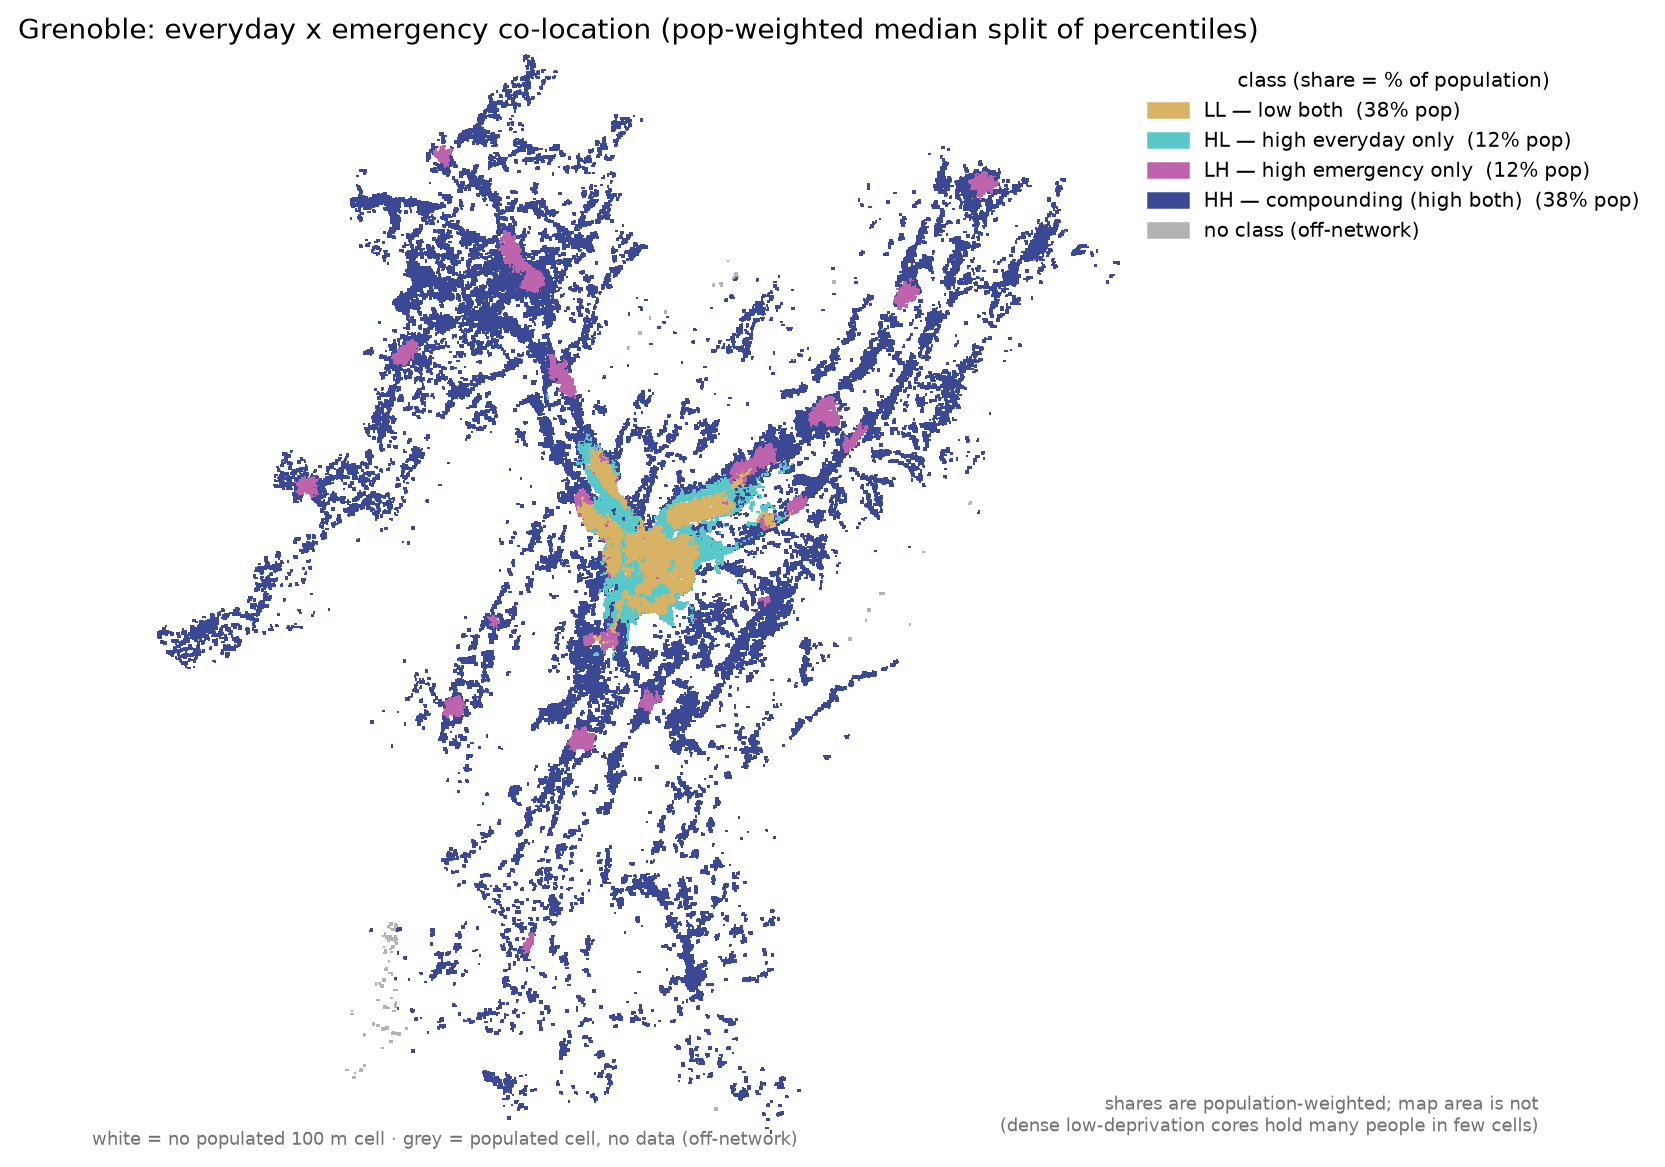
\includegraphics[width=0.48\textwidth]{grenoble.png}%
\\[2pt]
\caption{Per-city compounding maps (median-split co-location typology), cities 37--42 by population: Bratislava (SK), Ljubljana (SI), Palma de Mallorca (ES), Brno (CZ), Tallinn (EE), Grenoble (FR). Read for spatial pattern only; per-cell classes carry a $\sim$24\,\% routing-engine flip share (E.1).}
\label{fig:si-gallery-7}
\end{figure}

\begin{figure}[p]
\centering

\includegraphics[width=0.48\textwidth]{luxembourg.png}%
\hfill
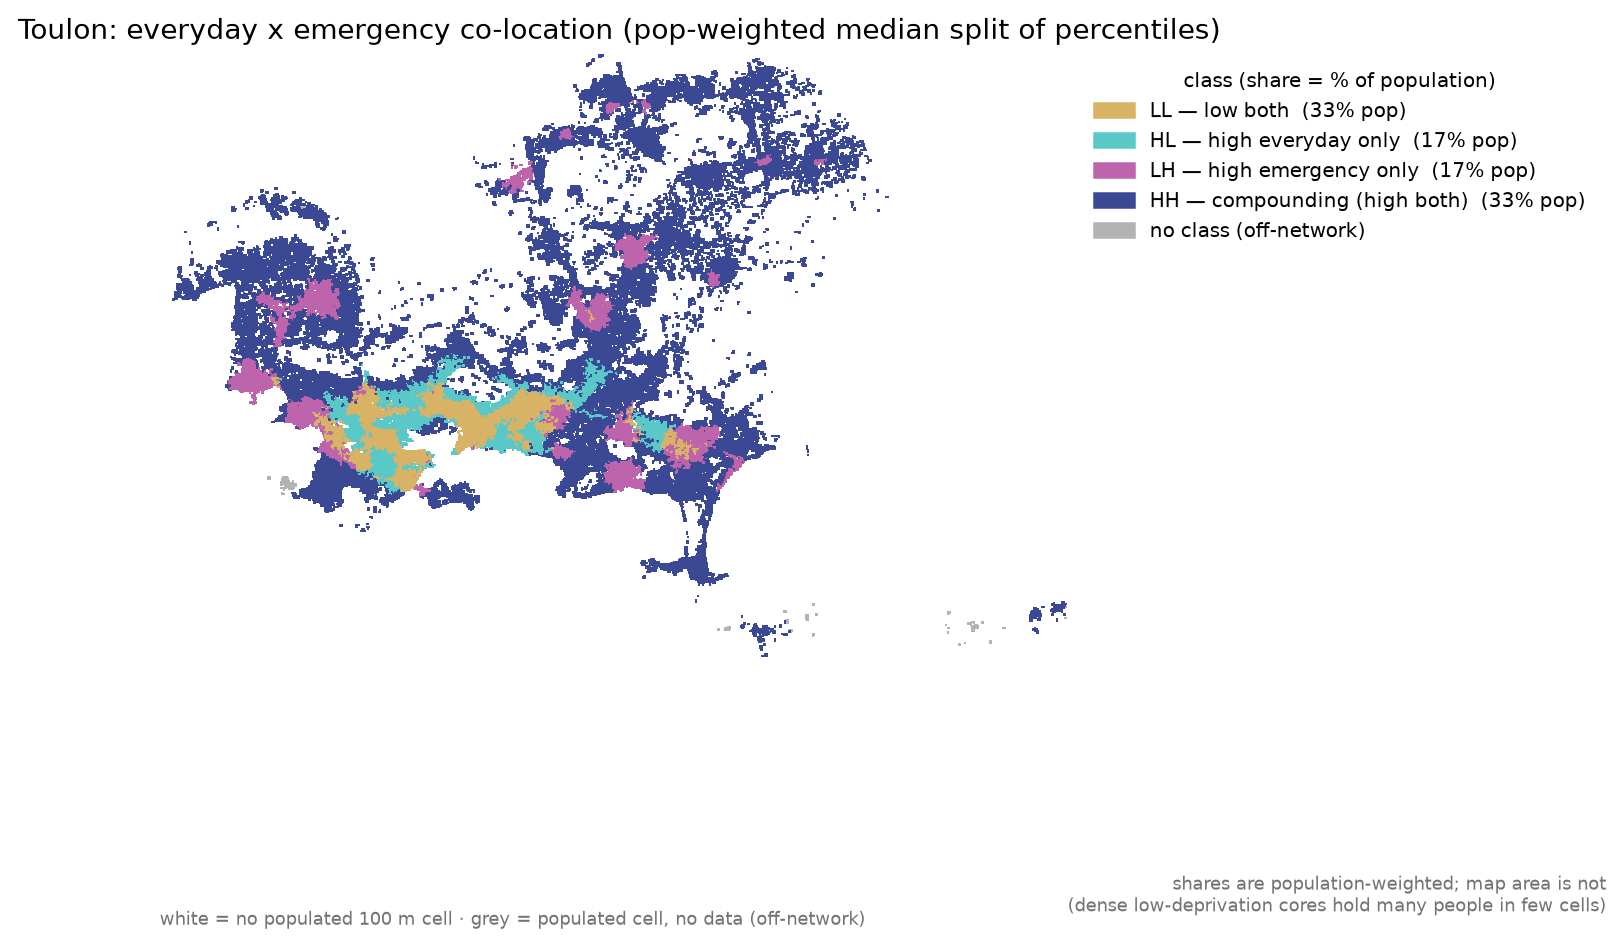
\includegraphics[width=0.48\textwidth]{toulon.png}%
\\[2pt]
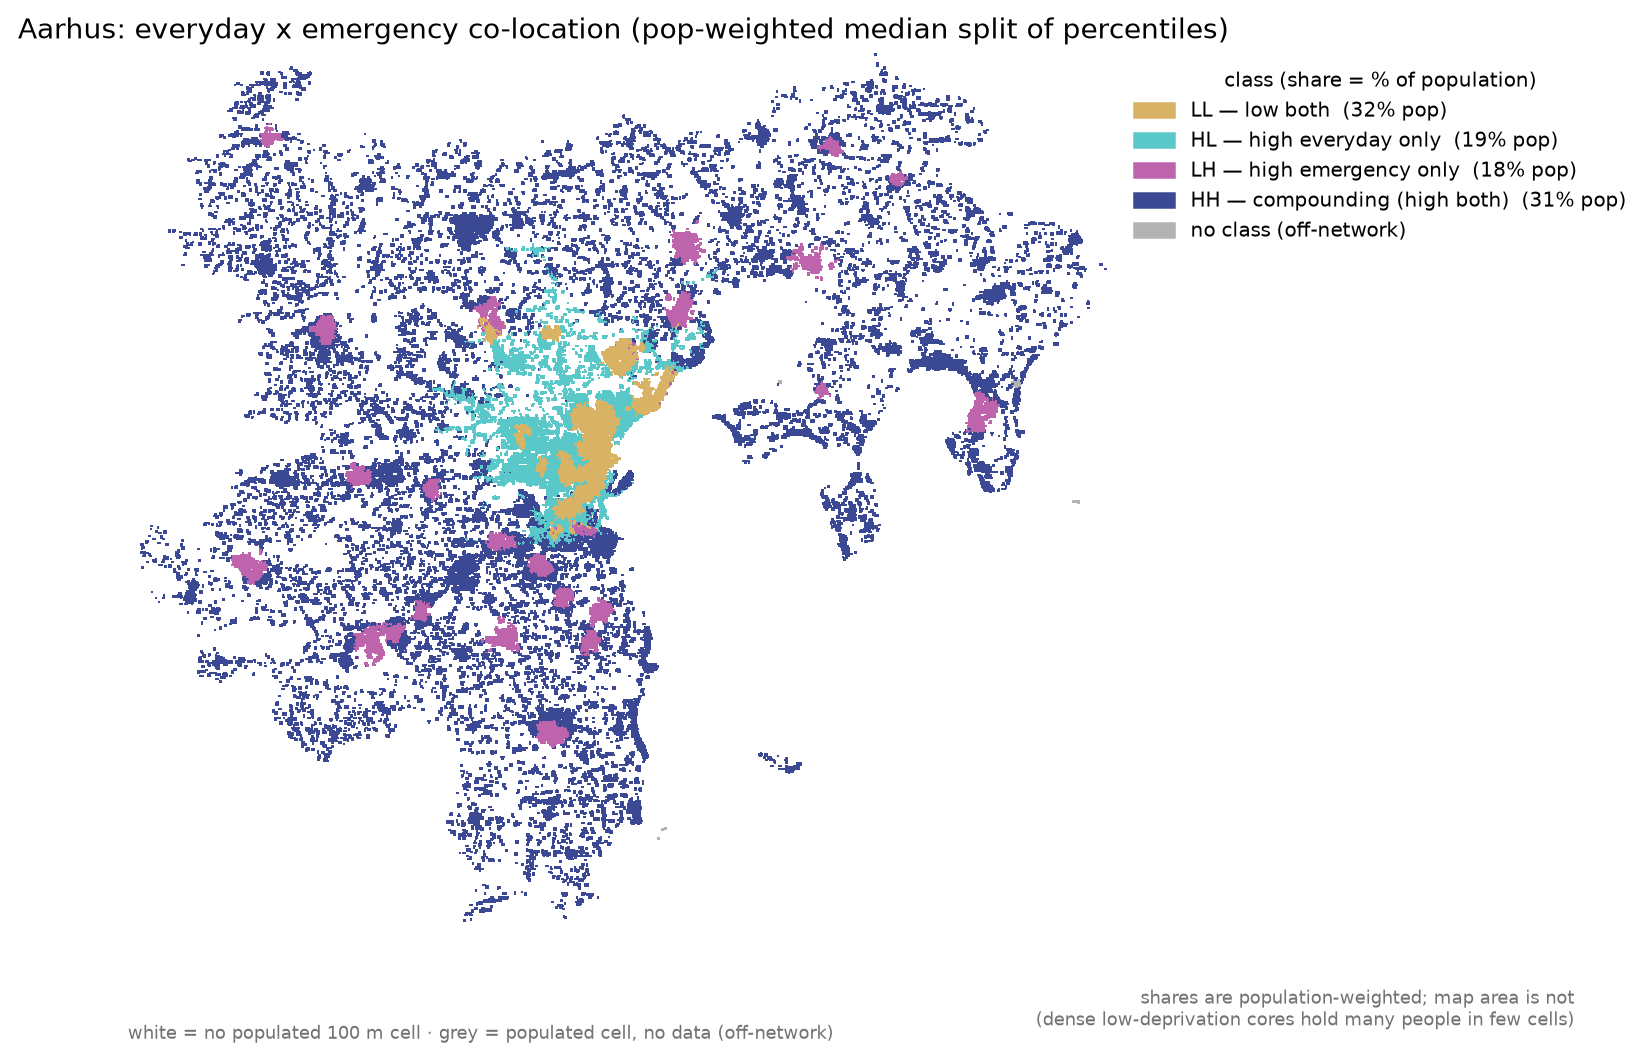
\includegraphics[width=0.48\textwidth]{aarhus.png}%
\hfill
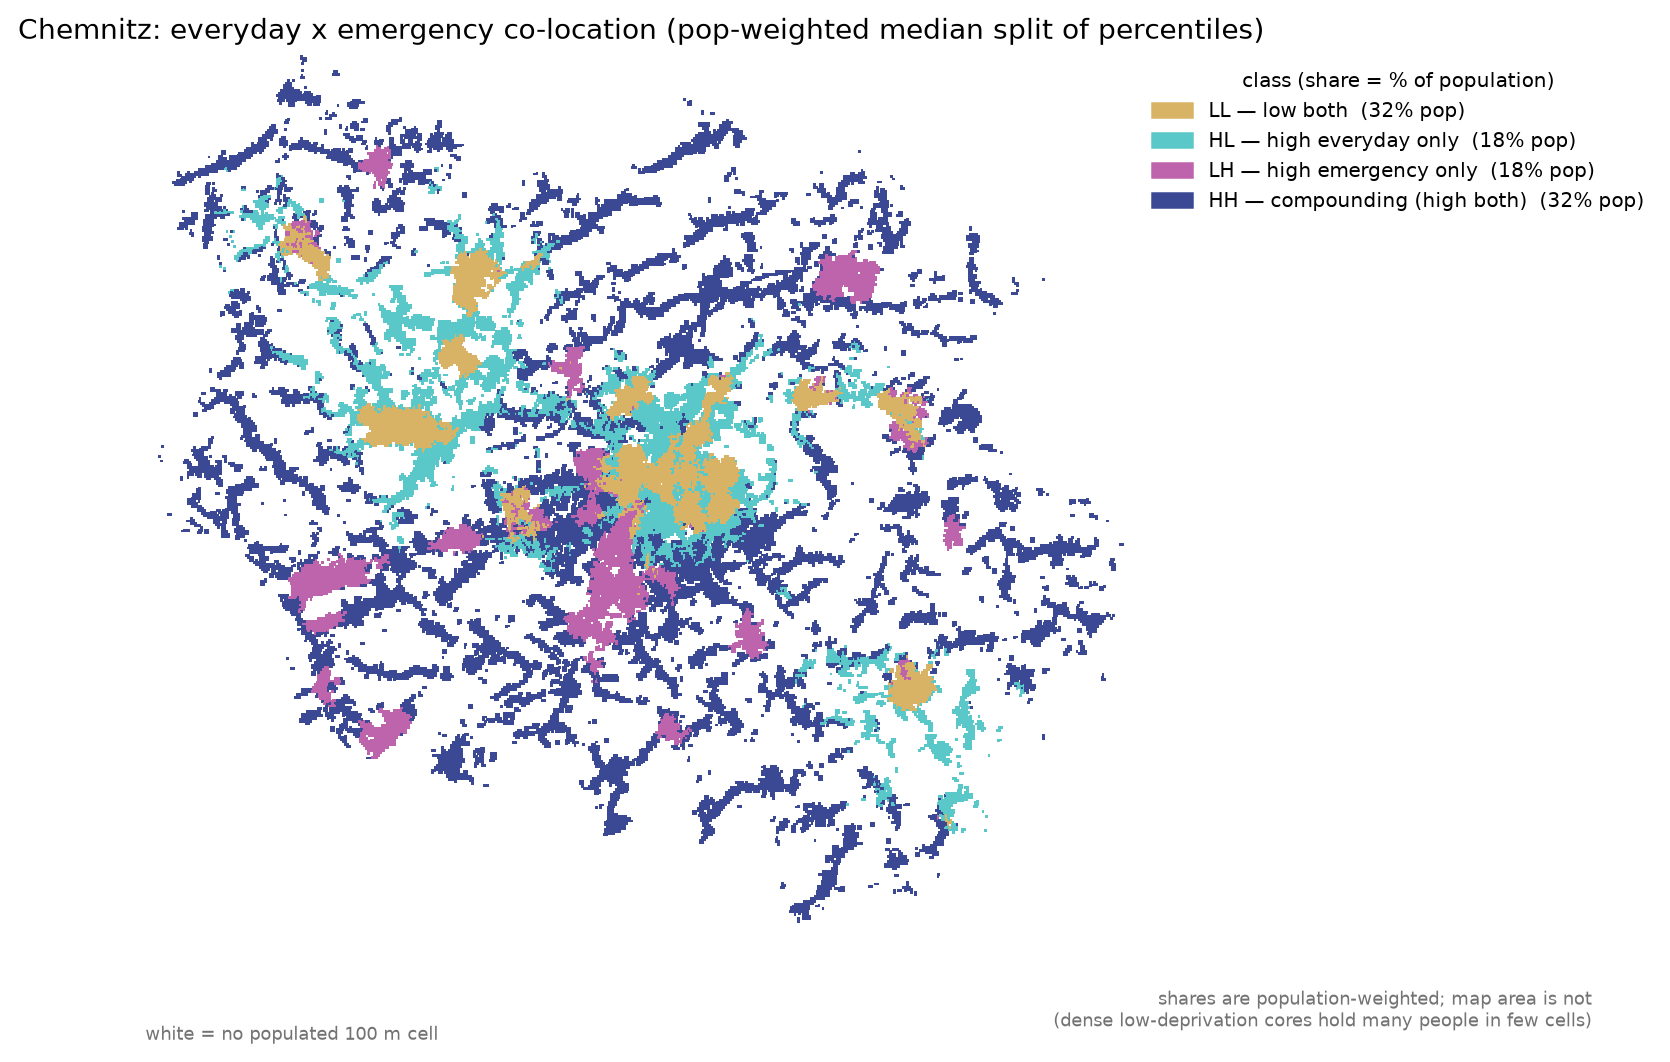
\includegraphics[width=0.48\textwidth]{chemnitz.png}%
\\[2pt]

\includegraphics[width=0.48\textwidth]{turku.png}%
\hfill

\includegraphics[width=0.48\textwidth]{stavanger.png}%
\\[2pt]
\caption{Per-city compounding maps (median-split co-location typology), cities 43--48 by population: Luxembourg (LU), Toulon (FR), Aarhus (DK), Chemnitz (DE), Turku (FI), Stavanger (NO). Read for spatial pattern only; per-cell classes carry a $\sim$24\,\% routing-engine flip share (E.1).}
\label{fig:si-gallery-8}
\end{figure}

\begin{figure}[p]
\centering

\includegraphics[width=0.48\textwidth]{aalborg.png}%
\hfill
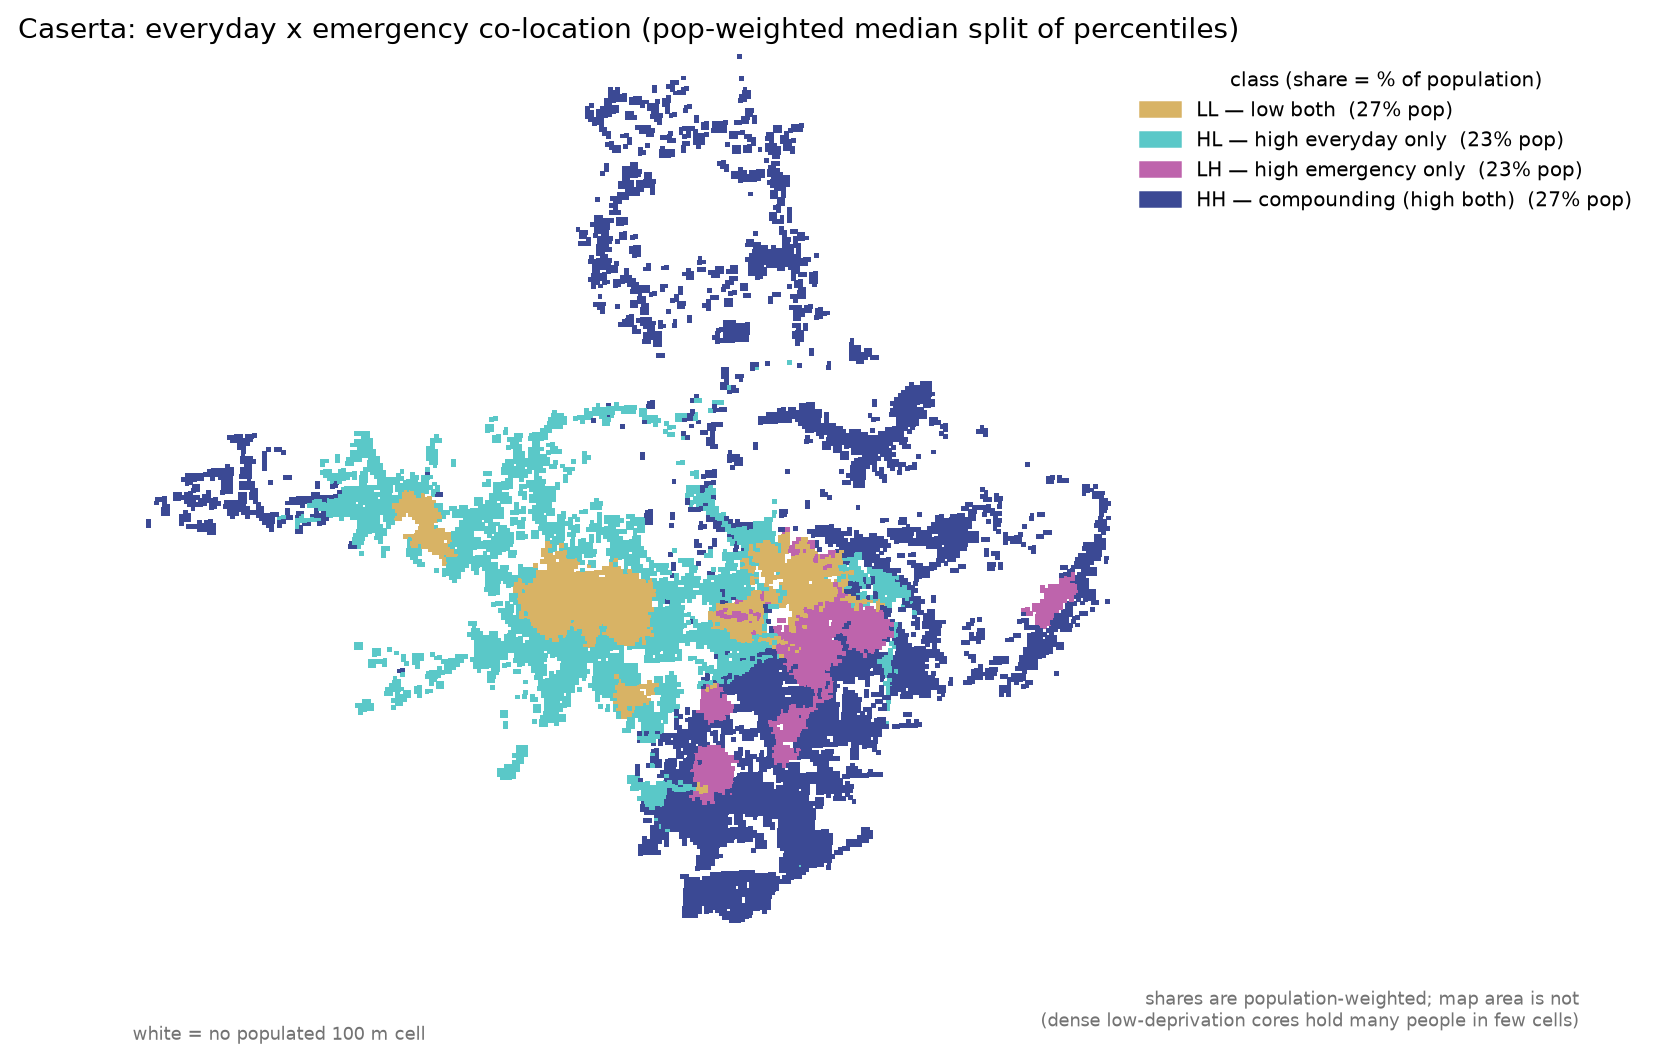
\includegraphics[width=0.48\textwidth]{caserta.png}%
\\[2pt]
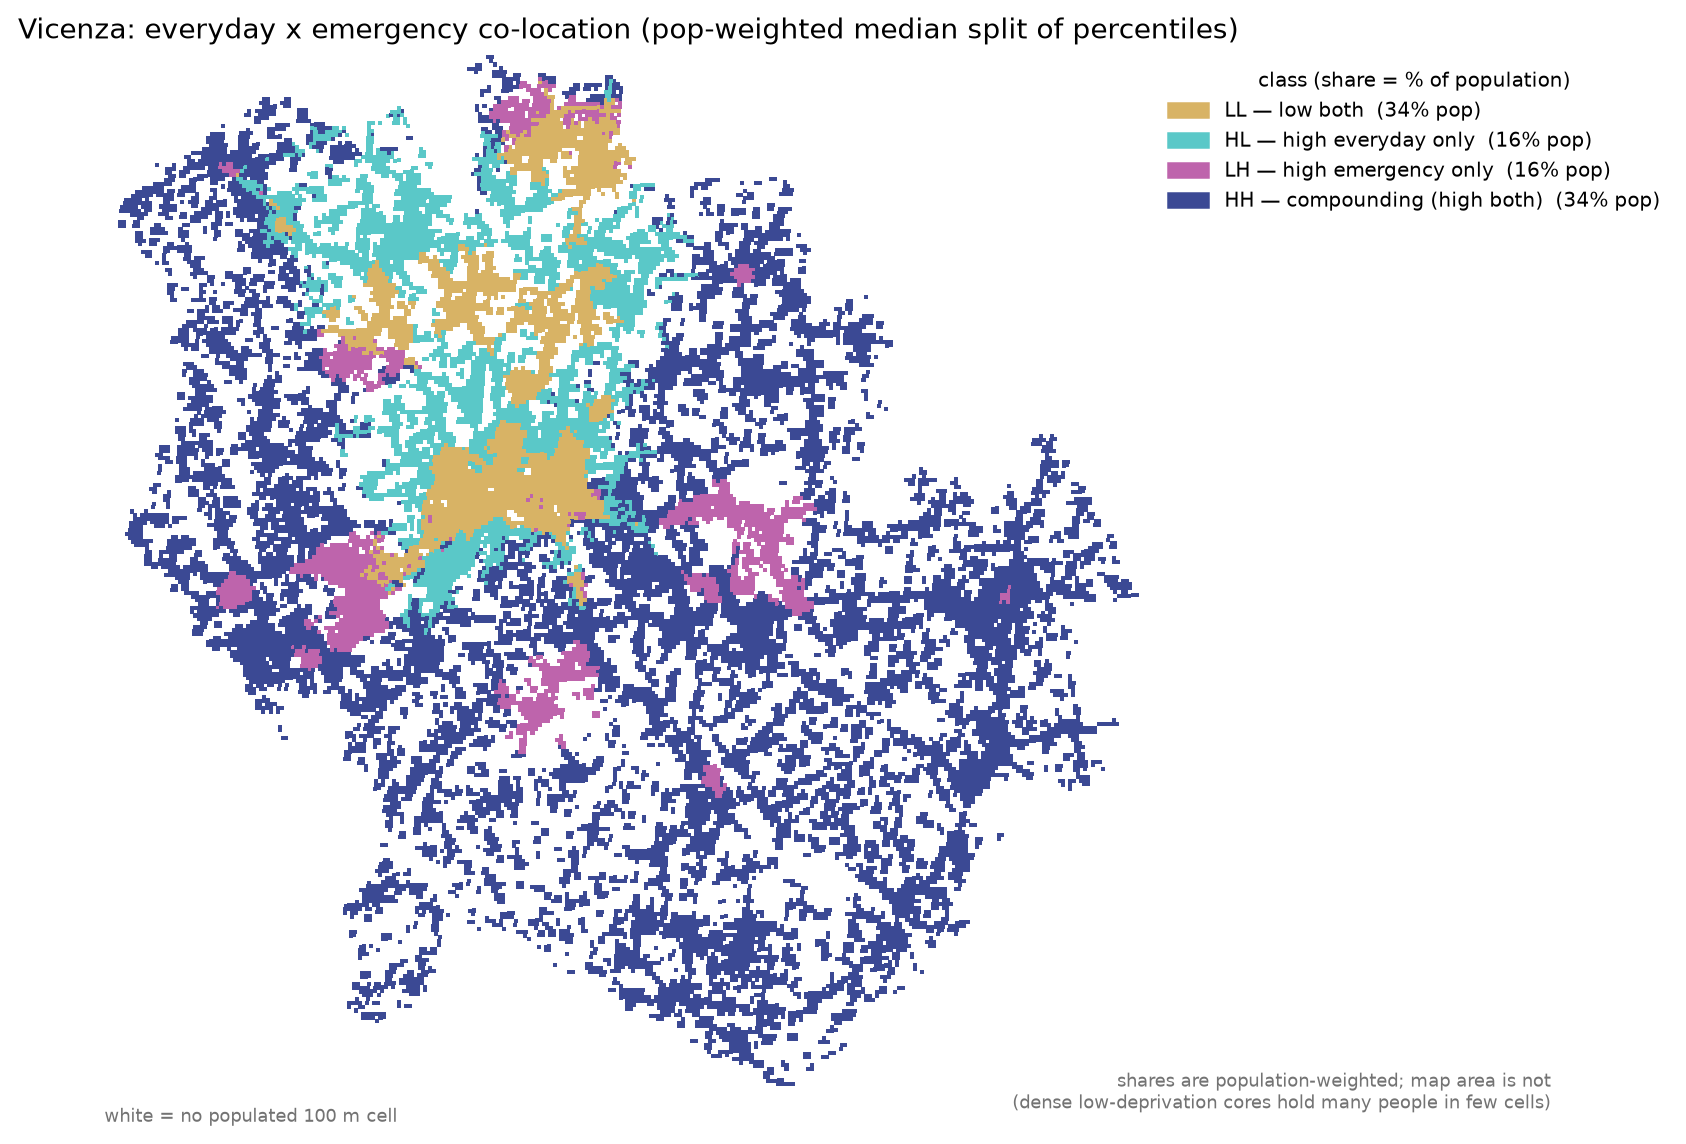
\includegraphics[width=0.48\textwidth]{vicenza.png}%
\hfill

\includegraphics[width=0.48\textwidth]{helsingborg.png}%
\\[2pt]
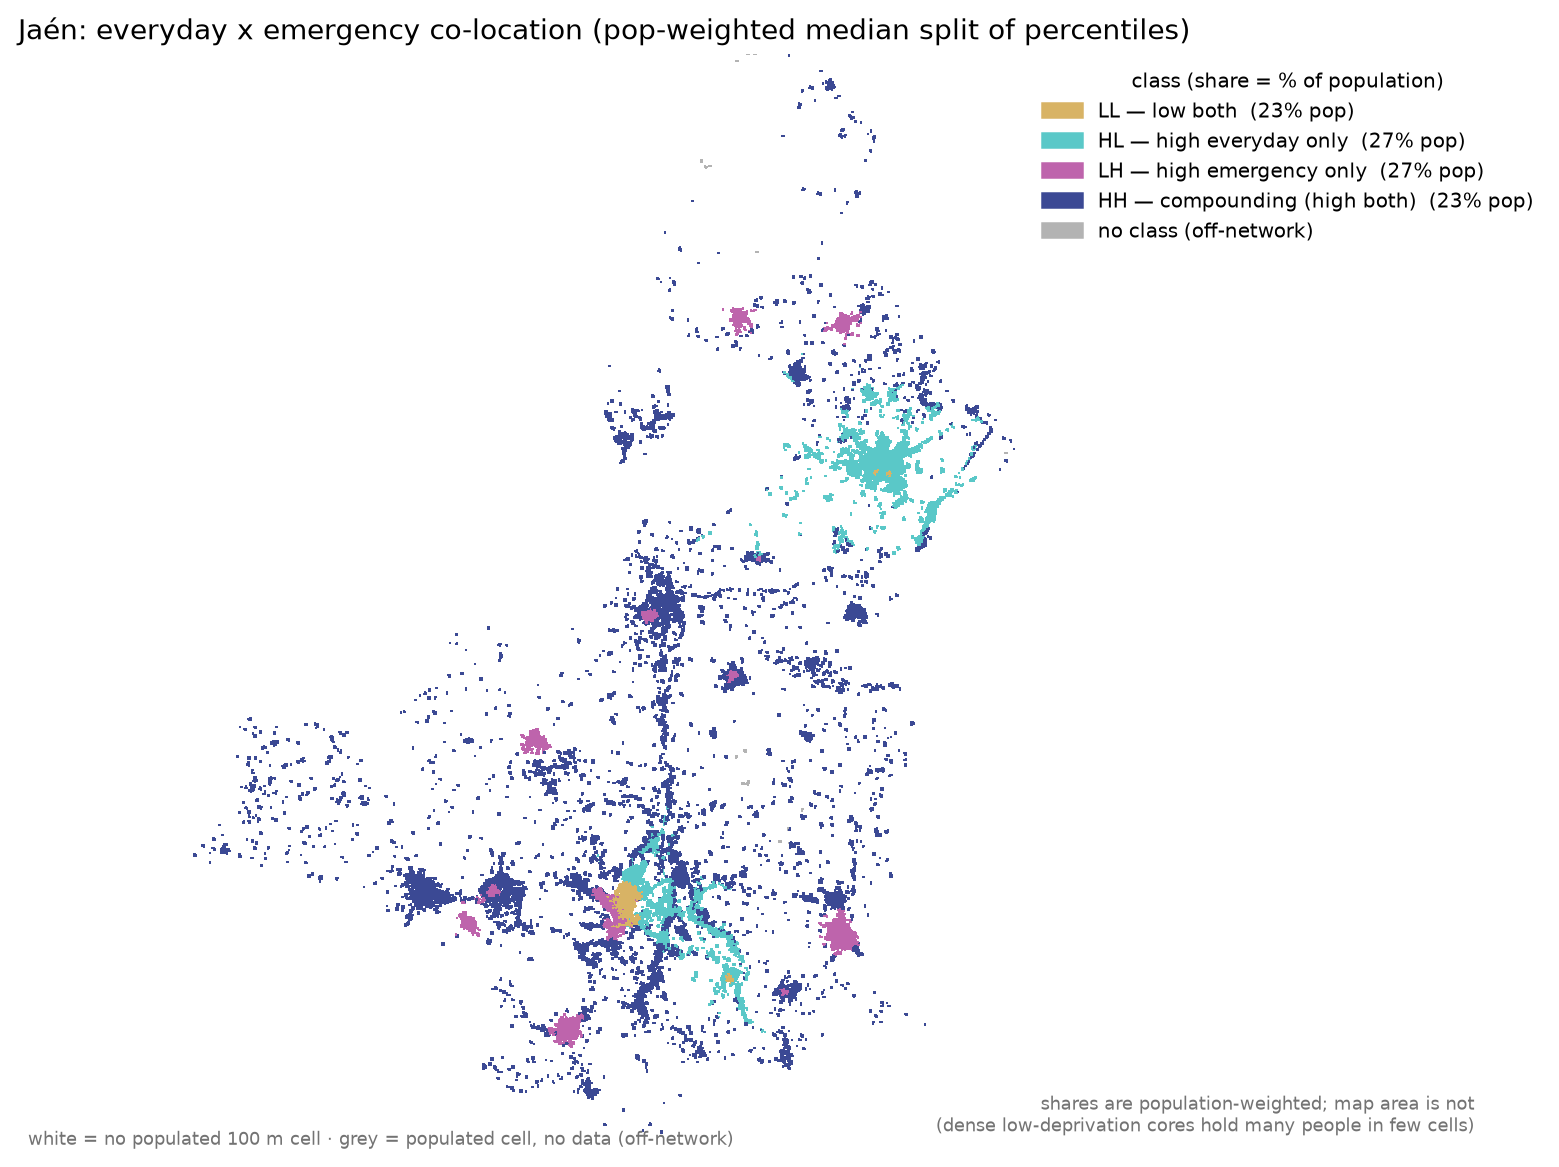
\includegraphics[width=0.48\textwidth]{jaen.png}%
\hfill
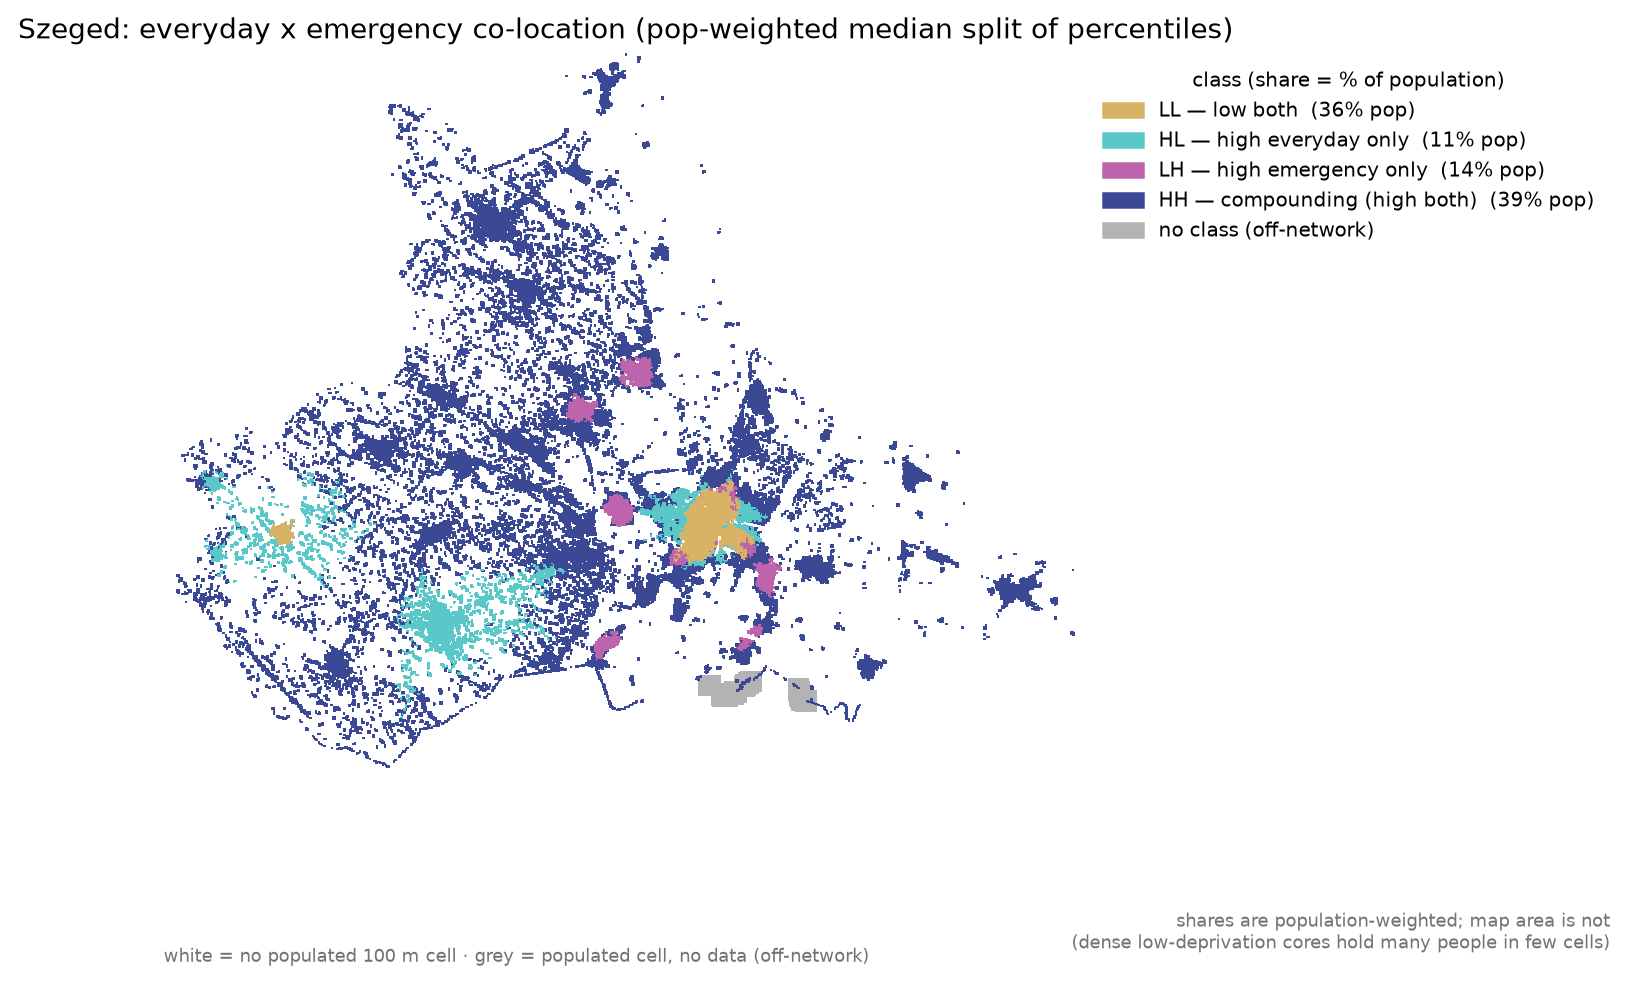
\includegraphics[width=0.48\textwidth]{szeged.png}%
\\[2pt]
\caption{Per-city compounding maps (median-split co-location typology), cities 49--54 by population: Aalborg (DK), Caserta (IT), Vicenza (IT), Helsingborg (SE), Ja{\'e}n (ES), Szeged (HU). Read for spatial pattern only; per-cell classes carry a $\sim$24\,\% routing-engine flip share (E.1).}
\label{fig:si-gallery-9}
\end{figure}

\begin{figure}[p]
\centering
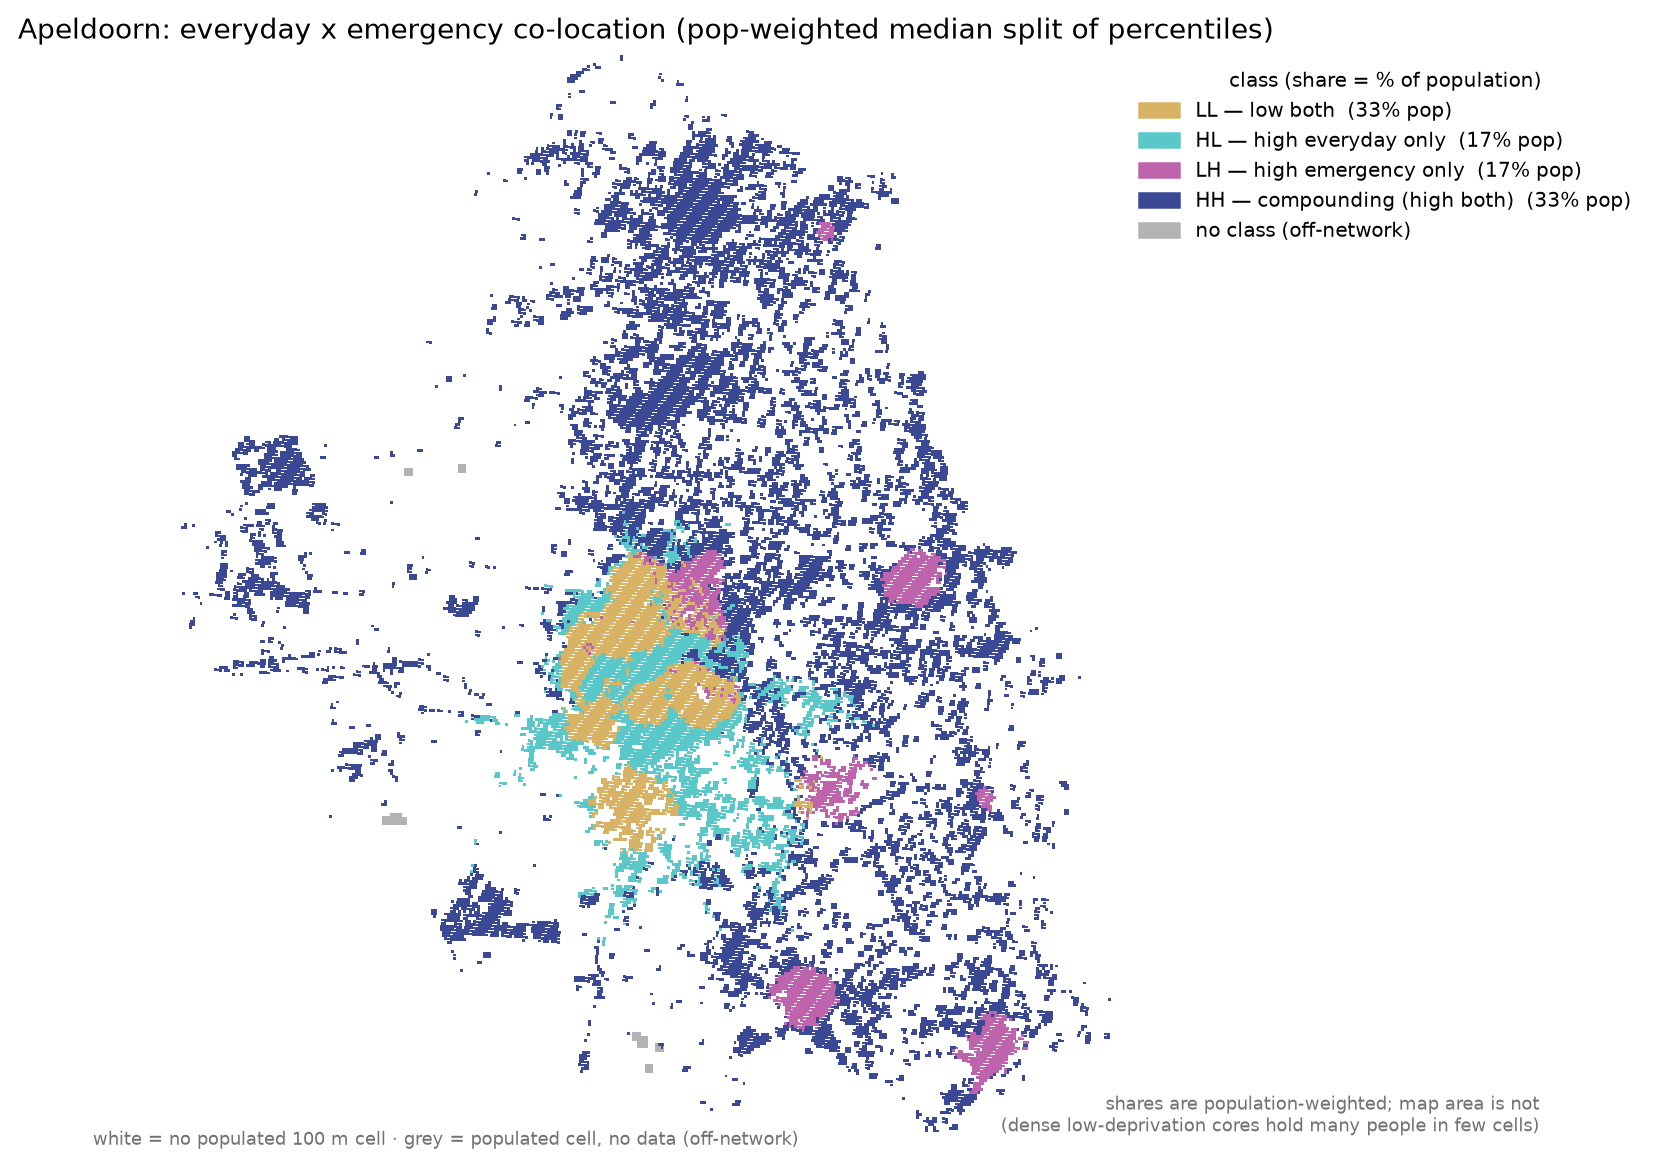
\includegraphics[width=0.48\textwidth]{apeldoorn.png}%
\hfill

\includegraphics[width=0.48\textwidth]{cosenza.png}%
\\[2pt]

\includegraphics[width=0.48\textwidth]{braila.png}%
\hfill

\includegraphics[width=0.48\textwidth]{amersfoort.png}%
\\[2pt]
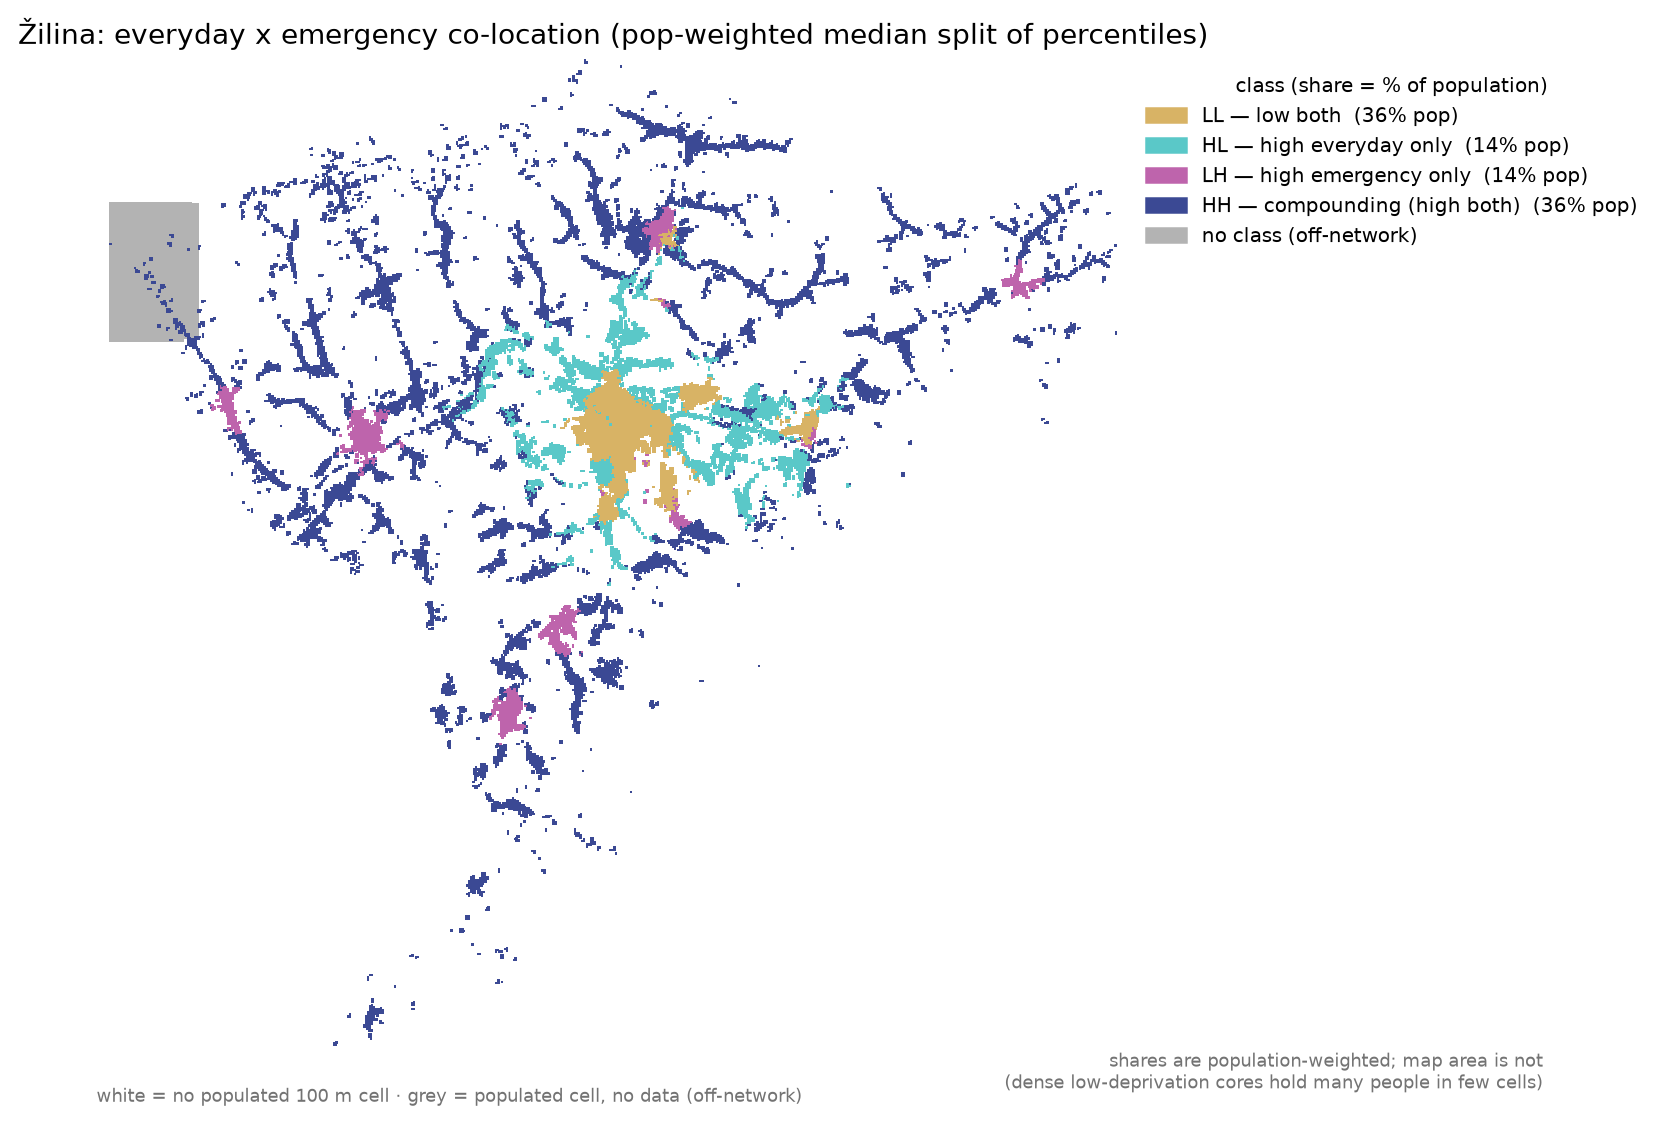
\includegraphics[width=0.48\textwidth]{zilina.png}%
\hfill

\includegraphics[width=0.48\textwidth]{vasteras.png}%
\\[2pt]
\caption{Per-city compounding maps (median-split co-location typology), cities 55--60 by population: Apeldoorn (NL), Cosenza (IT), Br{\u{a}}ila (RO), Amersfoort (NL), {\v{Z}}ilina (SK), V{\"a}ster{\r{a}}s (SE). Read for spatial pattern only; per-cell classes carry a $\sim$24\,\% routing-engine flip share (E.1).}
\label{fig:si-gallery-10}
\end{figure}

\begin{figure}[p]
\centering

\includegraphics[width=0.48\textwidth]{norrkoping.png}%
\hfill
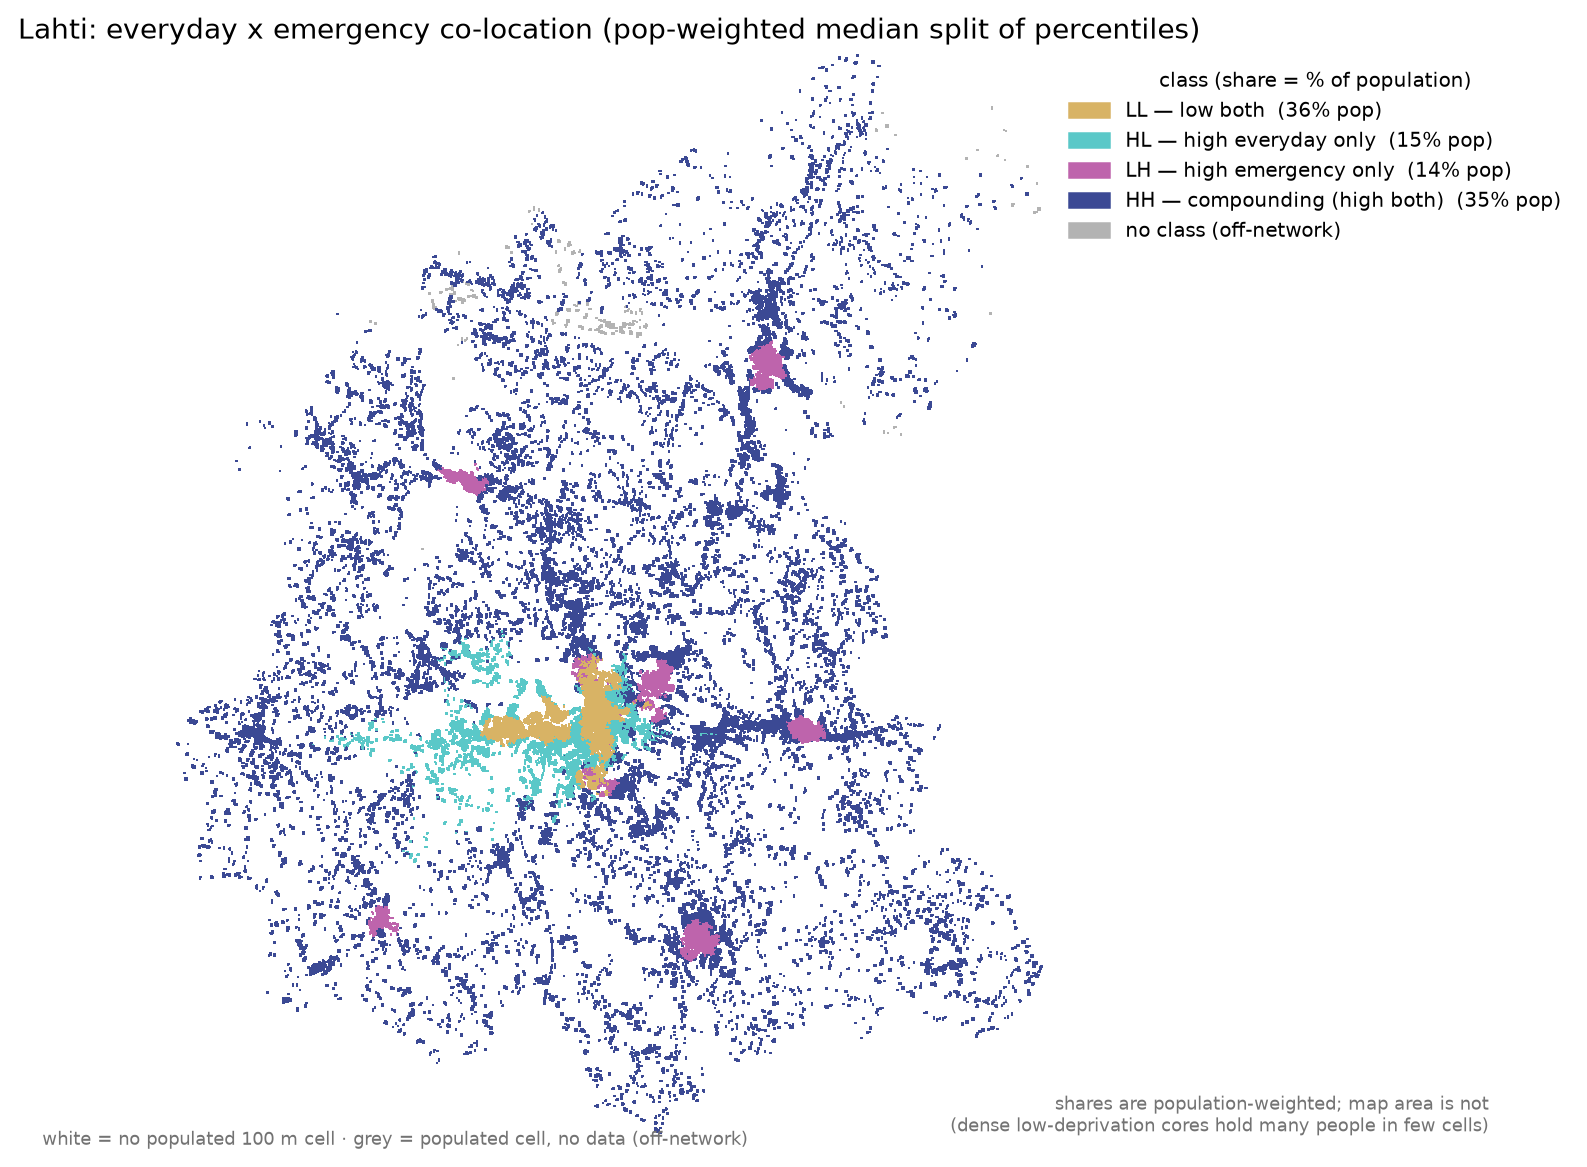
\includegraphics[width=0.48\textwidth]{lahti.png}%
\\[2pt]
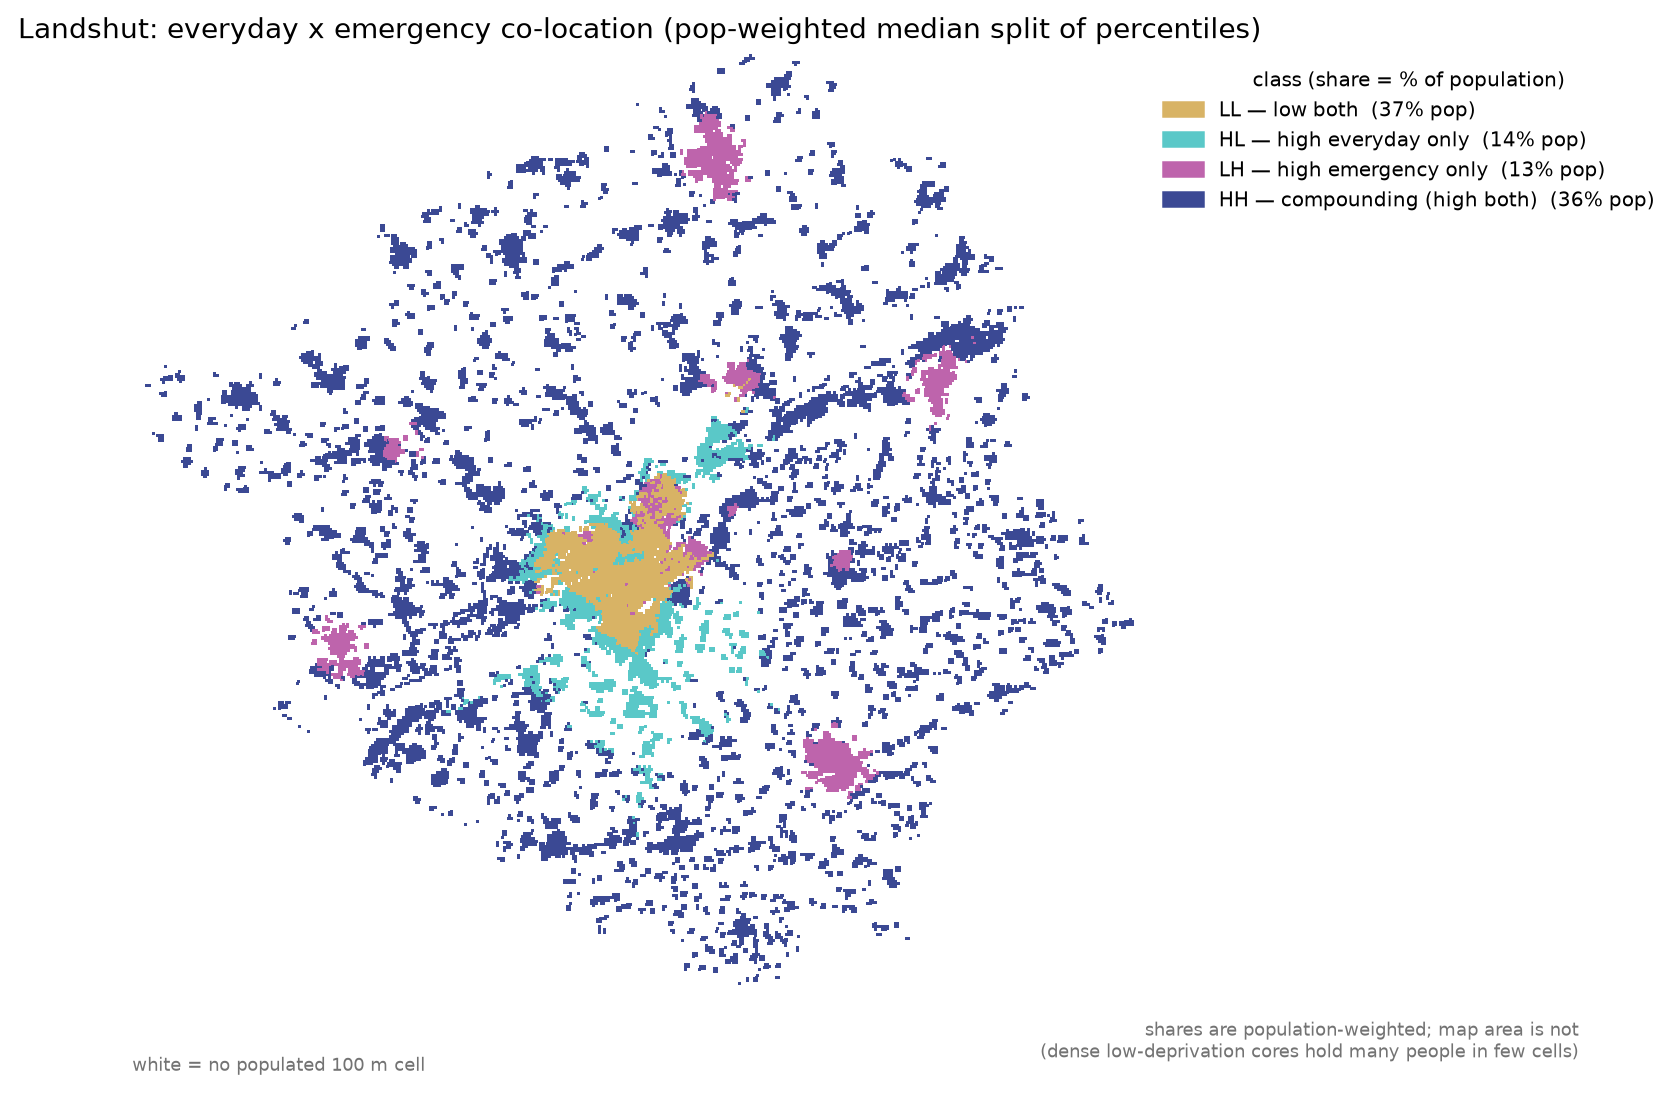
\includegraphics[width=0.48\textwidth]{landshut.png}%
\hfill
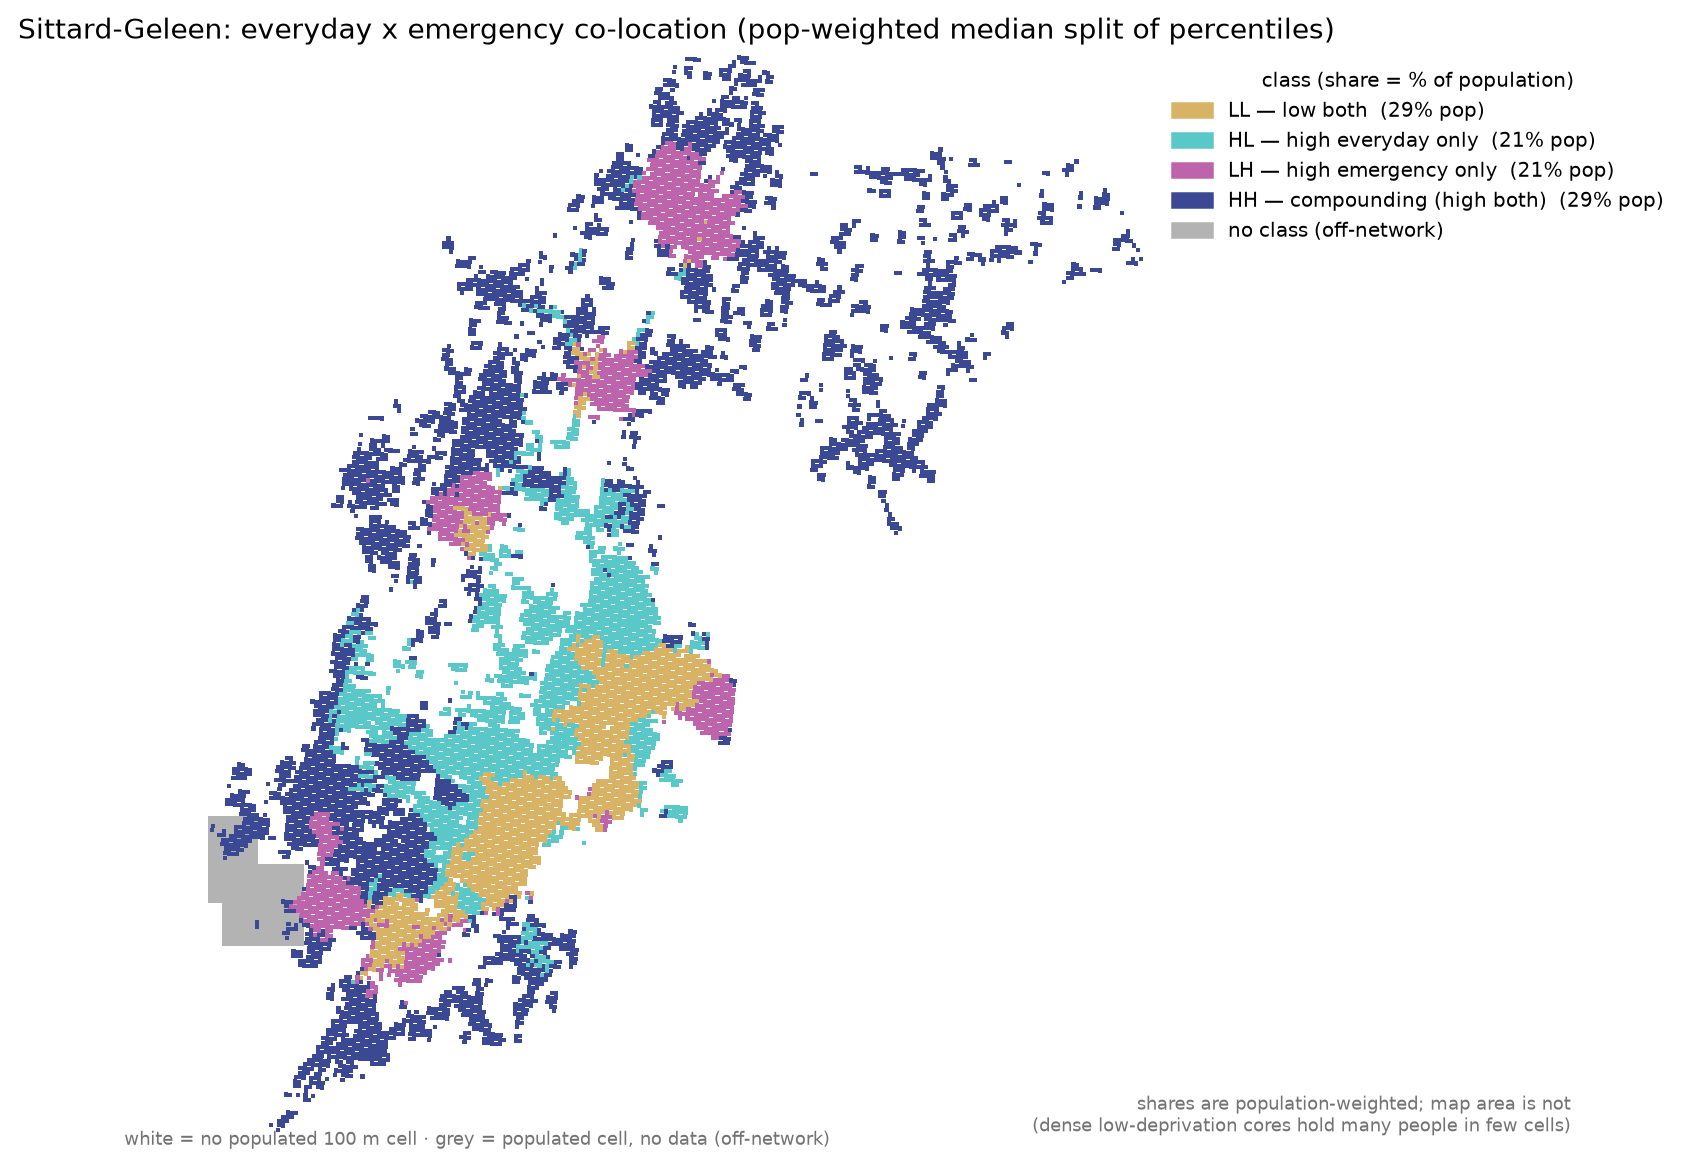
\includegraphics[width=0.48\textwidth]{sittard_geleen.png}%
\\[2pt]
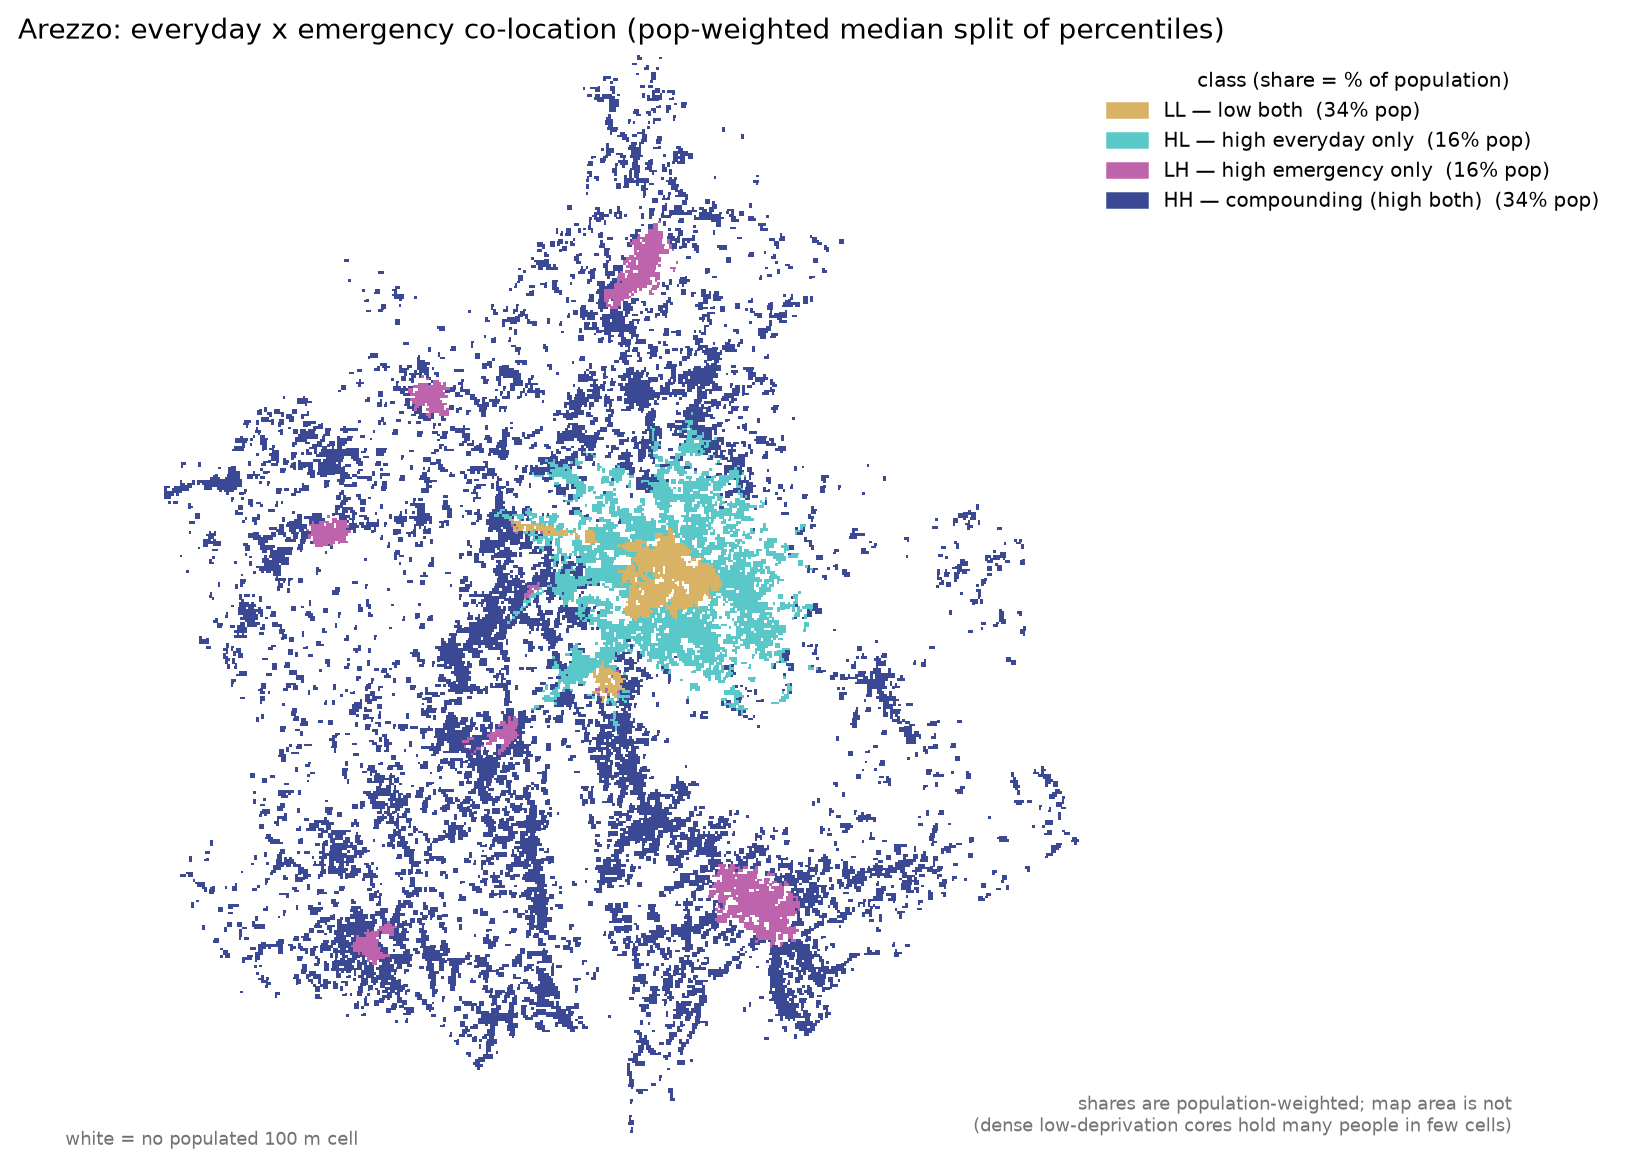
\includegraphics[width=0.48\textwidth]{arezzo.png}%
\hfill
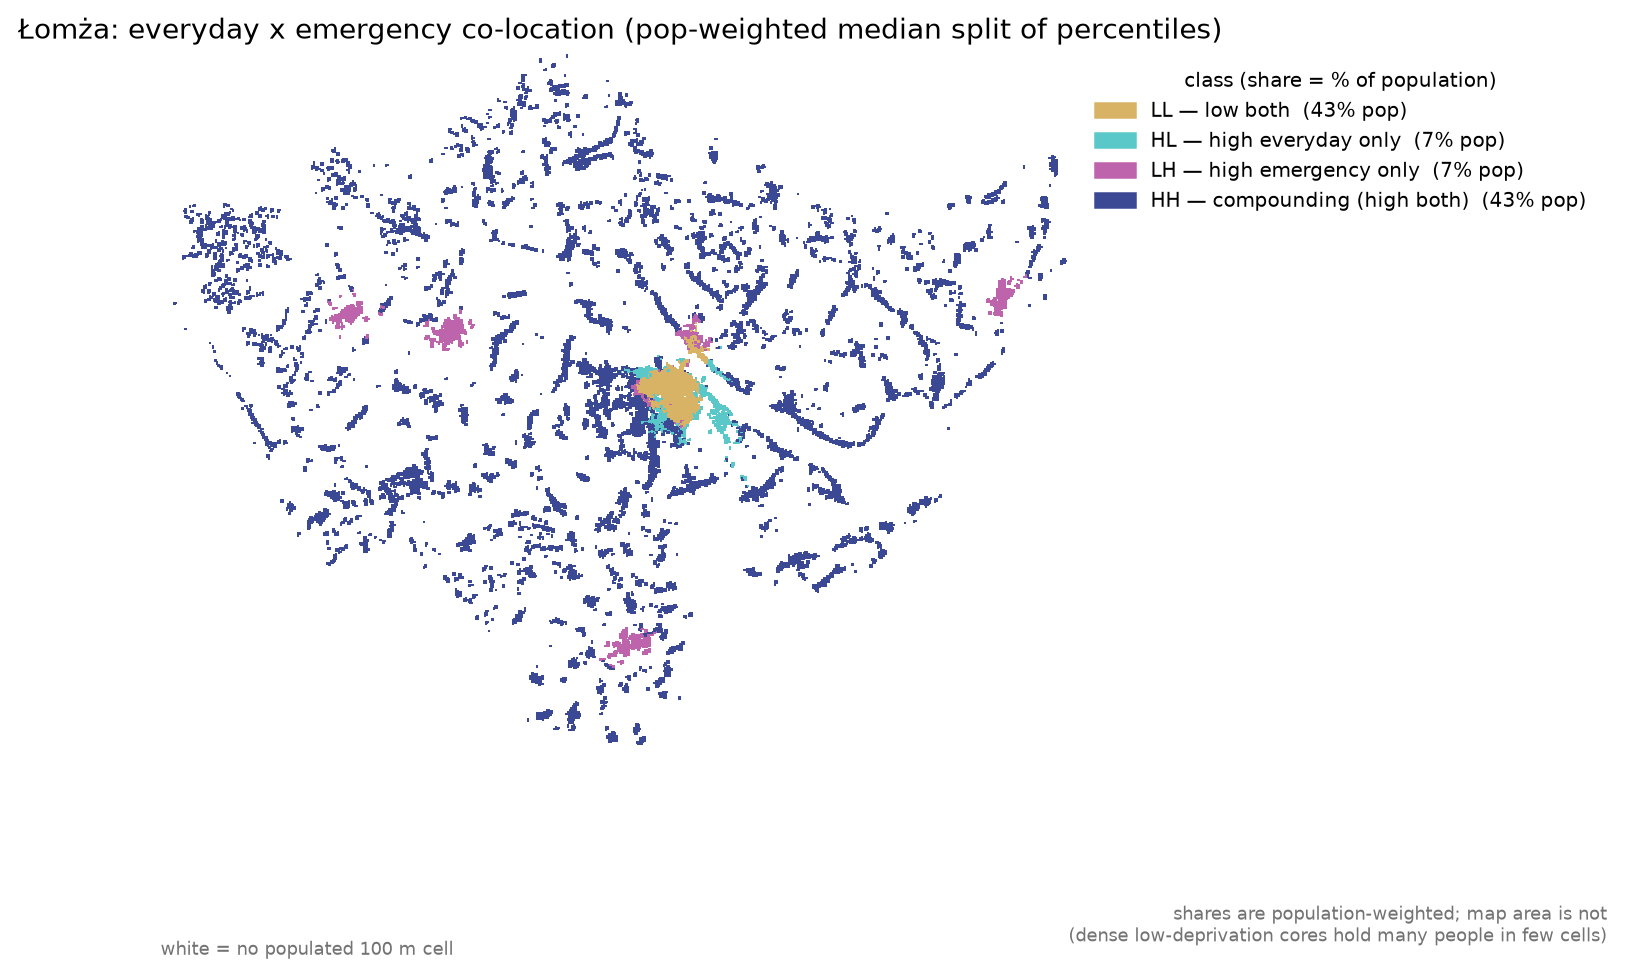
\includegraphics[width=0.48\textwidth]{lomza.png}%
\\[2pt]
\caption{Per-city compounding maps (median-split co-location typology), cities 61--66 by population: Norrk{\"o}ping (SE), Lahti (FI), Landshut (DE), Sittard-Geleen (NL), Arezzo (IT), {\L{}}om{\.z}a (PL). Read for spatial pattern only; per-cell classes carry a $\sim$24\,\% routing-engine flip share (E.1).}
\label{fig:si-gallery-11}
\end{figure}

\begin{figure}[p]
\centering
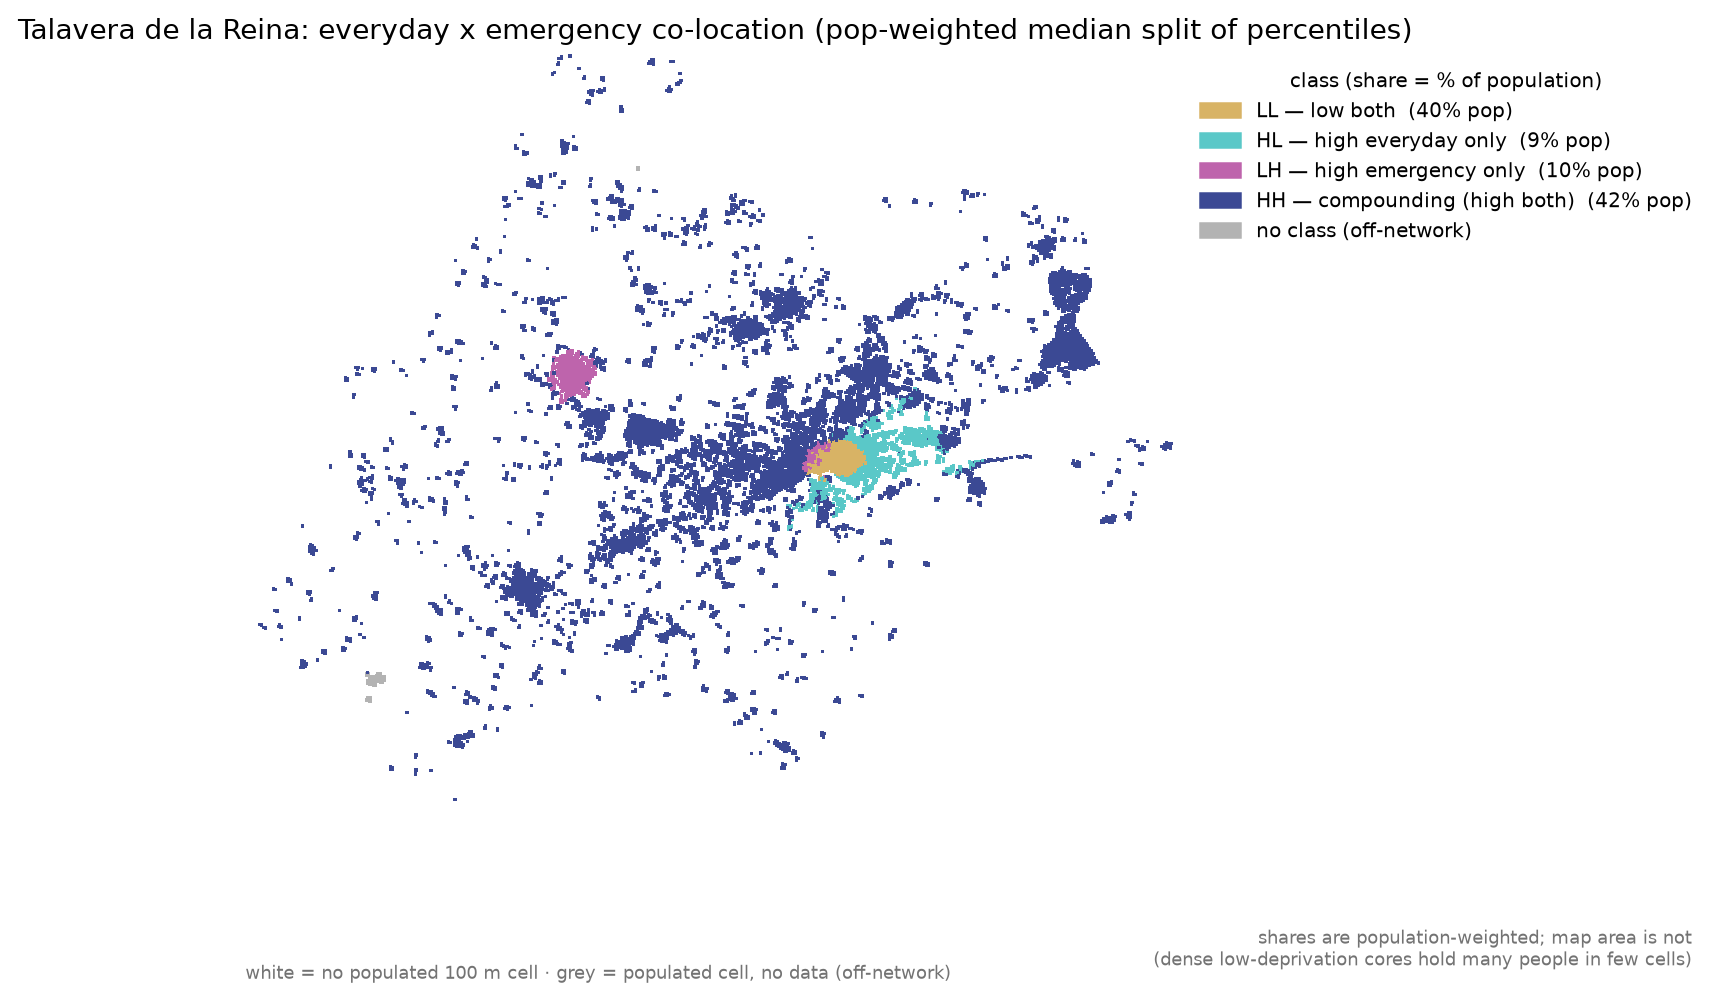
\includegraphics[width=0.48\textwidth]{talavera_de_la_reina.png}%
\hfill
\caption{Per-city compounding maps (median-split co-location typology), cities 67--67 by population: Talavera de la Reina (ES). Read for spatial pattern only; per-cell classes carry a $\sim$24\,\% routing-engine flip share (E.1).}
\label{fig:si-gallery-12}
\end{figure}



\end{document}
